
\chapter{Type System}

We have seen that ML style references are clumsy to work with because their use changes the structure of types. This causes mutable values to be type-incompatible with constant values, and invites large re-factorisation efforts when writing code. Could there be a better way? In a traditional imperative language such as C, Pascal or Java, the programmer is free to update data as they see fit, and the type of mutable data is not required to be structurally different from that which remains constant. However, if we were to allow the programmer to update any object in the system, without tracking it carefully, then we would have to assume that \emph{every} object was mutable. This would dramatically limit our ability to perform optimisations on the intermediate code. With this in mind, we first consider the form of update we wish to support, and then seek a way of tracking which objects it is applied to.

We intend this chapter to serve as a gentle introduction to our type system, and to the concepts involved. For this reason we have refrained from starting with a formal description of our language or its typing rules. This information is given in \S\ref{Inference:Language}.



% -------------------------------------
\section{Regions, Effects and Mutability Constraints}
In Haskell and ML, references and arrays are distinguished values, and are the only ones capable of being destructively updated. This means that the structure of mutable data is necessarily different from the structure of constant data, which makes it difficult to write polymorphic functions that act on both. For example, if we use $\iIORef \iInt$ as the type of a mutable integer and $\iInt$ as the type of a constant integer, then we would need $\ireadIORef$ to access the first, but not the second. On the other hand, if we were to treat all data as mutable, then every function would exhibit a side effect. This would prevent us from using code-motion style optimisations that depend on purity.

Instead, we give integers the type $\iInt \ r$, where $r$ is a region variable, and constrain $r$ to be mutable or constant as needed. Our use of region variables is similar to that by Talpin and Jouvelot \cite{talpin:type-and-effect-discipline}, where the variable $r$ is a name for a set of locations in the store where a run-time object may lie. We do not use regions for controlling allocation as per \cite{tofte:mlkit-4.3.0}, due to the difficulty of statically determining when objects referenced by suspended computations can be safely deallocated. We define region variables to have kind $\%$, and use this symbol because pictorially it is two circles separated by a line, a mnemonic for ``this, or that''. The kind of value types is *, so the $\iInt$ type constructor has kind $\iInt :: \% \to *$. The type of a literal integer such as `5' is:
\begin{tabbing}
MM	\= M \= M \= MMMM \kill
	\> 5	\> :: \> $\forall (r : \%). \iInt \ r$
\end{tabbing}
In our System-F style language, type application corresponds to instantiation, and `5' is the name of a function that allocates a new integer object into a given region. Note that unlike \cite{talpin:type-and-effect-discipline} we do not use allocation effects. This prevents us from optimising away some forms of duplicated computation, such as described in \S7 of \cite{benton:relational-semantics-effect-transformations}, but also simplifies our type system. For the rest of this paper we will elide explicit kind annotations on binders when they are clear from context.


% -------------------------------------
\subsection{Updating Integers}
\label{Update:UpdatingIntegers}

To update an integer we use the $\iupdateInt$ function which has type:
\begin{tabbing}
MM \= MMMMM \= MMMMMM \= MMMMM \= MMMM \kill
	\> $\iupdateInt$ \> $:: \forall r_1 \ r_2. 
				\iMutable \ r_1 
				\To \iInt \ r_1 \to \iInt \ r_2 
				\longtoa{\iRead r_2 \ \lor \ \iWrite r_1} ()$
\end{tabbing}
This function reads the value of its second integer argument, and uses this to overwrite the value of the first. As in \cite{talpin:type-and-effect-discipline} we annotate function types with their latent effects. We organise effects as a lattice and collect atomic effects with the $\lor$ operator. We use $\bot$ as the effect of a pure function, and unannotated function arrows are taken to have this effect. We also use a set-like subtraction operator where the effect $\sigma \setminus \sigma'$ contains the atomic effects that appear in $\sigma$ but not $\sigma'$. We use $!$ as the kind of effects, so $\iRead$ has kind $\iRead :: \% \to \ !$. The symbol ! is a mnemonic for ``something's happening!''.

Returning to the type of $\iupdateInt$, $\iMutable \ r_1$ is a \emph{region constraint} that ensures that only mutable integers may be updated. When we call this function we must pass a \emph{witness} to the fact that this constraint is satisfied, a point we will discuss further in \S\ref{Witnesses}.

When the number of atomic effects becomes large, using the above syntax for effects becomes cumbersome. Due to this we sometimes write effect terms after the body of the type instead:
\begin{tabbing}
MM \= MMMMM \= M \= MMMMM \= MMMM \kill
	\> $\iupdateInt$ 
		\> $::$	 	\> $\forall r_1 \ r_2. \iMutable \ r_1 \To \iInt \ r_1 \to \iInt \ r_2 \longtoa{e_1} ()$ \\
	\>	\> $\rhd$	\> $e_1$ = $\iRead \ r_2 \lor \iWrite \ r_1$
\end{tabbing}
The symbol $\rhd$ is pronounced ``with''. Note that the effect variable $e_1$ is not quantified. It has been introduced for convenience only and is not a parameter of the type. 


% -----------------------------------------------------------------------------
\subsection{Updating Algebraic Data}
Along with primitive types such as $\iInt$, the definition of an algebraic data type can also contain region variables. For example, we define our lists as follows:
\begin{tabbing}
MM \= MMMMM \= M \= MMMMM \= MMMM \kill
	\> $\kdata \ \iList \ r \ a = \iNil \ | \ \iCons \ a \ (\iList \ r \ a)$
\end{tabbing}
This definition is similar to the one from \S\ref{Introduction} except that we have also applied the $\iList$ constructor to a region variable. This variable identifies the region that contains the list cells, and can be constrained to be constant or mutable as needed. The definition also introduces data constructors that have the following types:
\begin{tabbing}
MM \= MMM \= M \= MMMMM \= MMMM \kill
	\> $\iNil$	\> $:: \forall r \ a. \ \iList \ r \ a$ \\
	\> $\iCons$	\> $:: \forall r \ a. \ a \to \iList \ r \ a \to \iList \ r \ a$  
\end{tabbing}
In the type of $\iNil$, the fact that $r$ is quantified indicates that this constructor allocates a new $\iNil$ object. Freshly allocated objects do not alias with existing objects, so they can be taken to be in any region. On the other hand, in the type of $\iCons$, the type of the second argument and return value share the same region variable $r$, which means the new cons-cell is allocated into the same region as the existing cells. For example, evaluation of the following expression produces the store objects shown below.

\begin{tabbing}
MM	\= MMMMMMM \kill
	\> $\ilist :: \iList \ r_5 \ (\iInt \ r_6)$ \\
	\> $\ilist = \iCons \ r_5 \ (\iInt \ r_6) \ (2 \ r_6) \ 
			(\iCons \ r_5 \ (\iInt \ r_6) \ (3 \ r_6) \ (\iNil \ r_5 \ (\iInt \ r_6)))$
\end{tabbing}

\begin{center}

\includegraphics[scale=0.6]{fig/list-regions.eps}
\end{center}

As the list cells and integer elements are in different regions, we can give them differing mutabilities. If the type of $\ilist$ was constrained as follows, then we would be free to update the integer elements, but not the spine.

\begin{tabbing}
MM	\= MMMMMMM \kill
	\> $\ilist :: \iConst \ r_5 \To \iMutable \ r_6 \To \iList \ r_5 \ (\iInt \ r_6)$
\end{tabbing}

The definition of an algebraic type also introduces a set of update operators, one for each updatable component of the corresponding value. For our list type, as we could usefully update the head and tail pointers in a cons-cell, we get the following operators:

\begin{tabbing}
MM \= MMMMMMx \= M \= MMMMM \= MMMM \kill
	\> $\iupdate_{Cons, 0}$	
		\> $:: \forall r \ a. \ \iMutable \ r \To \iList \ r \ a \to a \longtoa{\iWrite \ r} ()$ 
\\
	\> $\iupdate_{Cons, 1}$	
		\> $:: \forall r \ a. \ \iMutable \ r \To \iList \ r \ a \to \iList \ r \ a \longtoa{\iWrite \ r} ()$
\end{tabbing}

These operators both take a list and a new value. If the list contains an outer cons-cell, then the appropriate pointer in that cell is updated to point to the new value. If the list is not a cons, then a run-time error is raised.


\clearpage{}
\section{Region Typing}
\label{System:Regions}

% ---------------------
\subsection{Regions and aliasing}
A region is the set of store locations where a particular object may be present at runtime. We use regions to reason about the mutability and aliasing of objects. The following diagram shows a store containing a number of objects, divided into two regions. This diagram is intended to be suggestive only. Many systems besides our own make use of regions, and a particular system may allow them to be disjoint areas of the store, include free space, grow with time, be hierarchical, include only sub-components of an object, and so on.

\begin{center}
\includegraphics[scale=0.8]{2-System/fig/regions-inHeap}
\end{center}

We use $\rho_n$ to denote \emph{region handles}. A region handle can be thought of as a runtime identifier for a particular region, or perhaps an index into a table that describes the extent of a region. For the simple system in the diagram, we could treat a region as a set of aligned, 4-byte words. In this case our region handles could be defined as:


\code{
	$\rho_1$ & 	$ = \{ 1234, 1238, 1246, 1250 \}$ \\
	$\rho_2$ & 	$ = \{ 1682, 1690 \}$
}

At compile time we will not necessarily know how the objects in the store will be arranged, or how to define the region handles. We would like to write functions that operate on objects from any region, independently of how they are arranged. For this purpose we introduce \emph{region variables}, which we use to bind region handles. Region variables are identified as $r_n$ in this text.

There are conceptual similarities between region and value information. Consider the following statements of value:

\code{
	$23$ 	& $\mapsto \ < ... 10010 ... >$  \\
	$a$  	& $= 23$ \\
}

In the first statement, the numeral 23 represents an object in the store that includes a particular bit string. In the second statement we have used a \emph{value variable} to bind the numeral 23. We can think of regions as being akin to the objects in the store, region handles being akin to numerals, and region variables being like value variables. In this sense, regions are physical things, region handles are descriptions of them, and region variables are place holders for the handles.

Clearly though, regions and values are different kinds of things. As per tradition we use a star * to denote the kind of value types. Region kinds are denoted by a percent sign \%\footnote{Pictorially, \% is two circles separated by a line, a mnemonic for ``this, or that"}. In the concrete syntax we also use \% as a namespace qualifier, writing \texttt{\%rn} in place of $r_n$. This helps the parser, as well as being convenient for syntax highlighting text editors.

Unlike the system of Tofte and Birkedal \cite{tofte:region-inference}, ours deals only with region variables and not with the definition of region handles, or the layout of the store. Their system uses regions to manage the allocation of free space at run time, where ours uses regions as part of an analysis to guide compile time code optimisations.

Our analysis is type based. We add region variables to all type constructors which correspond to data objects that can be usefully updated. This includes constructors like $\iInt$, $\iBool$ and $\iList$, but not the function constructor $(\rightarrow)$ or the unit constructor $()$. The function constructor does not need one because the value of a function cannot be updated at runtime. The unit constructor does not need one because there is only one possible unit value.  

For example, a list of character pairs could have type:

\code{
 	$\ipairs$ & $:: \iList \ r_1 \ (\iPair \ r_2 \ (\iChar \ r_3) \ (\iChar \ r_4))$ \\
 	$\ipairs$ & $= [\iMkPair \ \texttt{'g'} \ \texttt{'o'}, \ \iMkPair \ \texttt{'b'} \ \texttt{'y'}, \ \dots ]$
}

In a top level signature such as this, if two type constructors have different region variables, such as $\iChar \ r_3$ and $\iChar \ r_4$, then the corresponding values are guaranteed to be represented by different run-time objects. However, in general these objects may \emph{alias}. For example, here is a function which creates a pair of integers:

\code{
	$\iintPair  :: \forall r_1 \ r_2 \ r_3. \ \iInt \ r_1 
			\to \iInt \ r_2 \to \iPair \ r_3 \ (\iInt \ r_1) \ (\iInt \ r_2)$ \\
 	$\iintPair  \ x \ y \ = \ \iMkPair \ x \ y$
}


As the region variables $r_1$, $r_2$ and $r_3$ are quantified in the type signature, we may pass the same integer object for both arguments of the function:

\code{
	$\ifive$ 	& $:: \iInt \ r_5$ 					\\
	$\ifive$ 	& $= 5$
}

\vspace{-1ex}
\code{
	$\ipairOfFives$	& $:: \iPair \ r_4 \ (\iInt \ r_5) \ (\iInt \ r_5)$ 	\\
	$\ipairOfFives$	& $= \iintPair \ \ifive \ \ifive$
}

Here, the region variables $r_1$ and $r_2$ of $\iintPair$ have been instantiated to $r_5$. This tells us that both elements of the pair may refer to the same heap object, and they will in this case. Note that in the body of $\iintPair$, the value variables $x$ and $y$ may also refer to the same object because we can pass the same one for both arguments.

In the type of $\ipairOfFives$, the region variable $r_4$ is fresh because the evaluation of $\iintPair$ will allocate a new object to represent the pair. Freshly allocated objects do not alias any existing objects.

Aliasing information is of fundamental importance when reasoning about destructive update, as any read or write actions performed on objects in one region will not be visible to the parts of a program that only deal with another. To use the language of \cite{reynolds:interference}, actions performed on disjoint regions do not \emph{interfere}.

In many cases the region variables attached to differently named type constructors will be distinct, but this is not required in general. In our $\ipairs$ example, all the list constructor cells are in one region, and all the pair cells are in another:

\smallskip
\begin{center}
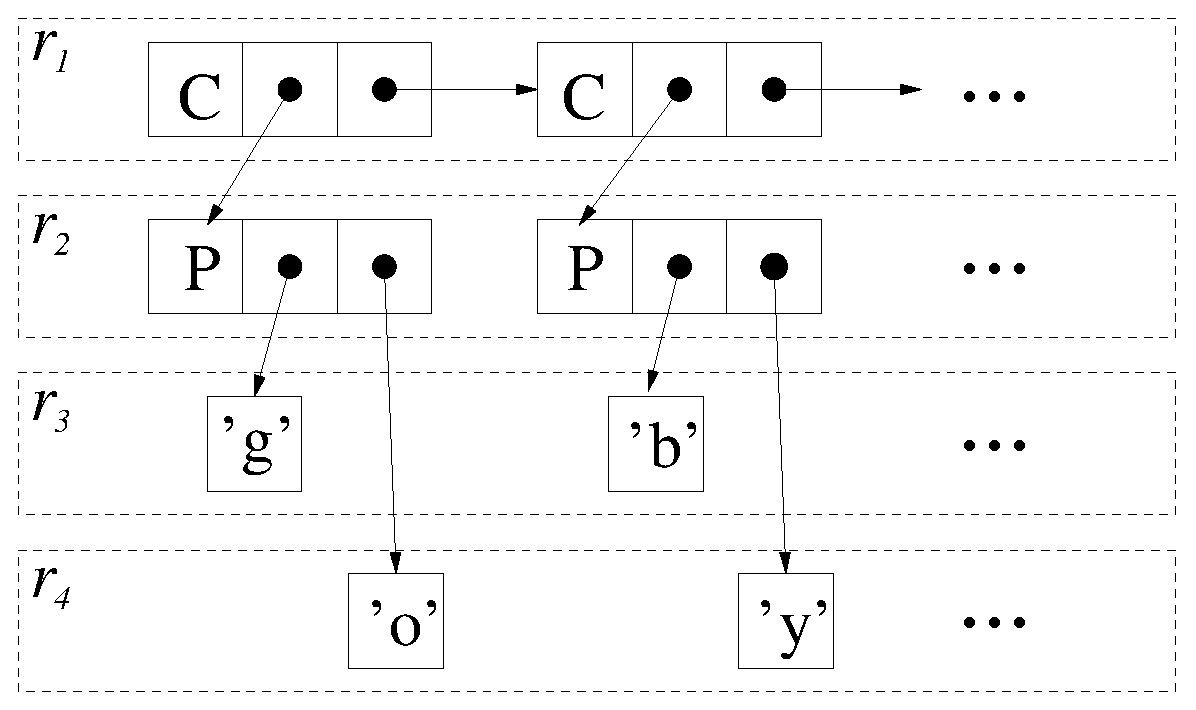
\includegraphics[scale=0.4]{2-System/fig/regions-list.eps}
\end{center}
\smallskip

Setting $r_1 = r_2$ would be equivalent to placing the list cells in the same region as the pair cells. 

Like Talpin and Jouvelot's original work \cite{talpin:discipline}, our concept of a region is simply a name for a set of locations. We sometimes find it useful to visualise regions as colours of paint, which we apply to data objects stored in the heap. Setting $r_1 = r_2$ corresponds to painting all the list and pair cells the same colour. They will be harder to distinguish afterwards, corresponding to a weakening of our analysis, but it will cause them no harm.

As region variables are provided as parameters to type constructors, the kinds of the constructors reflect this. $\iChar$ takes a region and produces a type. $\iList$ takes a region, a type, and produces a new type. $\iPair$ takes a region, two types, and produces a new type:

\code{
	$\iChar$ 	& $:: \% \to *$ \\
	$\iList$ 	& $:: \% \to * \to *$ \\
	$\iPair$ 	& $:: \% \to * \to * \to *$ 
}


% ---------------------------
\subsection{Region classes}
When a value is mutable we add mutability constraints to the region variables in its type. For example, if we wanted to update the characters in a string we would give it type:

\code{
 	$\istr :: \iMutable \ r_2 \Rightarrow \iList \ r_1 \ (\iChar \ r_2)$
}

The constraint $\iMutable \ r_2$ is a \emph{region class}. Region classes are similar to the value type classes in Haskell \cite{hall:type-classes}, such as $Show$ and $Eq$. With value type classes, the type constraint $Eq \ a$ requires $a$ to be a type that supports equality. Similarly, the region constraint $\iMutable \ r_2$ requires $r_2$ to correspond with a region that supports update.

When discussing our system we use the word ``type'' to refer to all the information in a signature, including value type information such as $\iList$ and $\iChar$, any constraints on variables, region information, as well as the effect and closure information we will discuss later. For this reason we also refer to both region classes and value type classes as simply ``type classes". Note that the programmer usually doesn't have to provide this additional information in type signatures. Most can be reconstructed by the type inferencer. This is discussed further in \S\ref{System:Projections:ambiguous} and \S\ref{Inference:Generalisation:late-constraints}.

Returning to the signature of $\istr$, we call term on the right of the $\Rightarrow$, the \emph{body} of the type. We call the value portion of the body is its \emph{shape}, because this information describes the overall structure of the object in the store.

As our types often contain a large number of constraints, we usually write them after the body, instead of before it as in Haskell:

\code{
	$\istr$ 
	& $::$		& $\iList \ r_1 \ (\iChar \ r_2)$ \\
    	& $\rhd$	& $\iMutable \ r_2$
}

The $\rhd$ is pronounced ``with'', and is written as \texttt{:-} in the concrete syntax. The difference between the above type and the original prefix form is purely syntactic, and our compiler accepts both.

In the above type, no constraint has been placed on $r_1$. If we wish to update the spine of the list as well as its characters, then this region must also be mutable. Multiple constraints are separated by commas:

\code{
	$\istr$ 
	& $::$		& $\iList \ r_1 \ (\iChar \ r_2)$ \\
    	& $\rhd$	& $\iMutable \ r_1$ \\
	& $,$		& $\iMutable \ r_2$
}

Being able to update the spine of a list is useful for operations such as inserting a new element into the middle of the list, as it allows us to change the tail pointers of existing cons cells.

On the other hand, if we wish to \emph{prevent} updates to the spine we could use the constraint $\iConst \ r_1$ to enforce this:

\code{
	$\istr$ 
	& $::$		& $\iList \ r_1 \ (\iChar \ r_2)$ \\
    	& $\rhd$	& $\iConst \ r_1$ \\
	& $,$		& $\iMutable \ r_2$
}

As there are two region variables in this type, both the spine and elements can have differing mutabilities. Attempting to constrain a region variable to be both $\iMutable$ and $\iConst$ results in a compile time type error. 


% ---------------------
\subsection{Functions, allocation and non-material regions}
\label{System:Regions:non-material}
In our system the successor function has the following signature:


\code{
 	$\isucc :: \forall (r_1 :: \%) \ (r_2 :: \%). \ \iInt \ r_1 \to \iInt \ r_2$
}

In this type we have included the kind of each region variable, but as in Haskell we can omit this information if it can be easily inferred. The variables $r_1$ and $r_2$ must have region kind because they are used as parameters to the $\iInt$ constructor, so we instead write:

\code{
 	$\isucc :: \forall r_1 \ r_2. \ \iInt \ r_1 \to \iInt \ r_2$
}

Starting with the $\iInt \ r_1$ term on the left of the arrow, the fact that $r_1$ is quantified indicates that $\isucc$ can operate on values from any region. On the right of the arrow, the fact that $r_2$ is quantified indicates that $\isucc$ can produce its output \emph{into} any region. This is possible because the function allocates a new $\iInt$ object each time it is called, and freshly allocated objects do not alias existing objects. Alternatively, if a function does not allocate its return value, then the region variables in its return type will not be quantified:

\code{
	& $x :: \iInt \ r_3$ \\
	& $x = 5$ 
	\\[1ex]
	& $\isameX :: () \to \iInt \ r_3$ \\
	& $\isameX \ () = x$ \\
}

In this example, $\isameX$ returns the same object every time it is called. This object comes from its environment, and is shared between all calls to it, hence $r_3$ must remain unquantified. Unquantified region variables can also appear on the left of an arrow. This happens when a function conflates its arguments with values from the environment:

\code{
	& $y :: \iInt \ r_4$ \\
	& $y = 23$ 
	\\[1ex]
	& $\ichooseY :: \iInt \ r_4 \to \iInt \ r_4$ \\
	& $\ichooseY z = \kif \ ... \ \kthen \ y \ \kelse \ z$ \\
}

The object returned by $\ichooseY$ could be either its argument $z$, or the shared object $y$. Our system cannot represent the fact that the returned object might be in one region \emph{or} another, so we use the same variable for both. This limitation is discussed in \S\ref{Evaluation:Limitations:blocked-regions}. In this example, $r_4$ is also present in the environment, so it cannot be quantified in the type of $\ichooseY$. 

Although $r_4$ appears in the types of both $y$ and $\ichooseY$, each occurrence has a slightly different meaning. In the type of $y$, it represents a particular set of locations in the heap, and one of those locations contains the integer object of value 23. On the other hand, the use of $r_4$ in the type of $\ichooseY$ does not mean that $\ichooseY$ also contains an integer object. Instead, these occurrences represent locations in the store where the function's argument and return values lie. We distinguish between these two cases by saying that $r_4$ in the type of $y$ is in a \emph{material} position, whereas in the type of $\ichooseY$ is not. The difference between the material and immaterial positions of type constructors is discussed more fully in \S\ref{System:Closure:non-material-regions}.


% ---------------------
\subsection{Updating data requires it to be mutable}
\label{System:Regions:update}
When a function can update its argument, we add a constraint to its type that requires the argument to be mutable. For example, the $inc$ function destructively increments its argument and has type:

\code{
	$\iinc$ 	
	& $::$		& $\forall r_1. \ \iInt \ r_1 \to ()$ \\
    	& $\rhd$	& $\iMutable \ r_1$ \\
}

This type indicates that $\iinc$ can operate on integers in any region, as long as that region is mutable. We treat mutability as a capability provided by the objects in our system, and the requirement for this capability flows from the functions that make use of it. An alternative setup would be to explicitly \emph{permit} update by requiring the programmer to supply type signatures and mutability constraints for every object that is to be updated, or to use a special keyword when allocating them. We feel that the use of a special keyword would create clutter in the program, though we will sometimes require mutability constraints to be given in a type signature. We will return to this in \S\ref{Inference:Generalisation:late-constraints}.

During type inference, the compiler compares all the constraints placed on the region variables in the program. In the absence of an explicit type signature, if a particular region is not constrained to be mutable, then at runtime the objects contained within that region will never be passed to a function that can update them. For this reason, material region variables that are not constrained to be mutable are considered to be constant.

This does not apply to quantified, immaterial regions in the types of functions. In this case the three options: mutable, constant, and unconstrained, have distinct meanings. For example, in the following type signature:

\code{
 	$\ifoo :: \forall r_1. \ \iInt \ r_1 \to ()$
}

As $r_1$ is unconstrained we may apply this function to integers which are either mutable or constant, whereas with:

\code{
 	$\ifoo'$
	& $::$		& $\forall r_1. \ \iInt \ r_1 \to ()$ \\
	& $\rhd$	& $\iConst \ r_1$
}

We can only apply this function to integers which are constant.


% ---------------------
\subsection{Primary regions and algebraic data}
In all examples so far, the type constructors used have had only one region parameter. This is typical for simple types with a small amount of internal structure, but we need more when defining algebraic data. Consider a vector of two integers:

\code{
	\mc{2}{$\kdata \ \iIntVector \ r_1 \ r_2 \ r_3$} \\
	& $= \iIV \ (\iInt \ r_2) \ (\iInt \ r_3)$
}

The first region variable $r_1$ corresponds to the region containing the outer $\iIV$ constructor. This is called the \emph{primary region variable}. The variables $r_2$ and $r_3$ appear in the body of the definition and represent the regions containing the integer components. For example, the value $(\iIV \ 2 \ 3)$ would be represented as:

\smallskip
\begin{center}
\includegraphics[scale=0.5]{2-System/fig/regions-intVector.eps}
\end{center}

These three separate region variables provide three degrees of freedom when deciding which parts of the object should be mutable and which should be constant. Allowing $r_2$ and/or $r_3$ to be mutable permits the components to be updated, and when $r_1$ is mutable we can update the pointers in the outer constructor. The \emph{tag} of the outer constructor is also contained in the primary region. Updates to the tag permit the value of enumerations such as $\iBool$ to be changed. 

Note that with this system it is not possible to give the \emph{pointers} to the two components separate region variables. We omit this capability to reduce the complexity of the system, though we see no fundamental barrier to supporting it if required in the future.



% --------------------
\subsection{Thinking about regions}
There are several ways to conceptualise what a region actually ``is'', and we have mentioned two so far. Firstly, a region is an area of the heap where objects can be stored at runtime. For systems that use regions to manage allocation and deallocation \cite{tofte:mlkit-4.3.0}, this is the most natural. Fresh objects are allocated into a particular region, and the whole region is reclaimed by the storage manager when the objects contained are no longer needed by the running program. Such systems use region allocation to augment or replace the standard garbage collection mechanism. At an operational level, the regions in such systems are usually contiguous, or are constructed with a linked list of contiguous memory pages. However, DDC does not use regions to manage allocation, it relies on a traditional garbage collector. We can still imagine a region to be a specific area of the heap, but the parts of the heap that make up the region are scattered throughout, and do not form a contiguous block.

Secondly, a region is a label for a collection of objects in the store. Earlier we suggested imagining these labels to be like colours of paint. When a program is compiled, the compiler decides on a fixed set of colours (regions). It then pretends that at runtime, every object allocated by the program will be painted with one of these colours. The colours help it to reason about what the program is permitted to do with a certain object. For example, we could paint all the mutable objects with shades of pink, and all the constant objects with shades of blue. Importantly though, the colours are just pretend. Our analysis is static, so we do not record what region an object belongs to in the object itself, or maintain any region information at runtime.

Finally, a region is a label for a set of program points which perform allocation \cite{pierce:atapl}. If we know that a particular object is in region $r_1$, then it must have been allocated by one of the points corresponding to $r_1$. Every object is allocated by one program point, and an allocation point can allocate zero or more objects. Allocation points exist within functions, so whether or not an allocation point ever allocates depends on whether the function is ever called. However, during evaluation the objects tend to get mixed up, such as when choosing between two objects in an if-expression. This means that the compiler will usually lose track of the exact point where a particular object was allocated. It can only hope to reduce it to a small set of possibilities.  Using this idea we can imagine that if a region variable is constrained to be $\iConst$, some part of the program requires an allocation point to produce a constant object. Likewise, if a region variable is constrained to be $\iMutable$, some part of the program requires a mutable object. A mutability conflict arises when a particular allocation point must produce an object that is both mutable and constant. This is not possible, so we report an error. We will exploit this line of reasoning further when we come to prove the soundness of our core language in \S\ref{Core:Language:Soundness}.



\clearpage
\section{Effect typing}
\label{System:Effects}

% --------------------
\subsection{Effects and interference}
\label{System:Effects:interference}
When the evaluation of an expression performs read or write actions on mutable data, the compiler must ensure that these actions occur in the correct order, else the meaning of the program will change. We have seen how region variables are used to reason about the \emph{mutability} of data, and we now discuss how to reason about the actions. Following Talpin and Jouvelot \cite{talpin:discipline} we use \emph{effect typing} to annotate function types with a description of the actions each function performs. 

For example, the $\iinc$ function reads its argument, computes the successor, and writes the new value back to its argument. Adding this information to the type gives us:

\code{
 	$\iinc$ 
	& $::$		& $\forall r_1. \ \iInt \ r_1 \lfuna{\iRead \ r_1 \ \lor \ \iWrite \ r_1} ()$ \\
	& $\rhd$	& $\iMutable \ r_1$
}

The effect annotation on the function arrow tells us which regions in the store will be accessed when it evaluates. When the effect term becomes large this syntax is hard to read. For this reason we usually introduce an \emph{effect variable}, and add a constraint to the type that contains the original effect term:

\code{
	$\iinc$ 
	& $::$		& \mc{2}{$\forall r_1. \ \iInt \ r_1 \funa{e_1} ()$} \\
	& $\rhd$	& $e_1 = \iRead \ r_1 \lor \iWrite \ r_1$ \\
	& ,	 	& \mc{2}{$\iMutable \ r_1$}

}

Effect variables are identified as $e_n$ in this text, and as variables preceded by an exclamation mark\footnote{a mnemonic for: ``something's happening!"} \texttt{!en} in the concrete syntax. The exclamation mark is used as both a namespace qualifier and as the symbol for effect kinds. In the concrete syntax, effect constructors such as \texttt{!Read} and \texttt{!Write} are also preceded by this namespace qualifier. Akin to value type constructors, the effect constructors have specific kinds. Both $\iRead$ and $\iWrite$ take a region and produce an effect, so we have:

\code{
	$\iRead$	& $:: \% \to \ !$ \\
	$\iWrite$	& $:: \% \to \ !$
}

Treating the function constructor as a general type constructor, we can read the infix application $a \funa{e} b$ as shorthand for the prefix application $(\to) \ a \ b \ e$. This will help when presenting the typing rules of the core language, as we can use general type application to build function types instead of requiring a rule specific to functions.

Single, \emph{atomic effects} such as $\iRead \ r_1$ and $\iWrite \ r_1$ are gathered together with the join operator $\lor$. Effects form a lattice ordered by set inclusion on atomic effects. We use $\sigma_1 \sqsubseteq \sigma_2$ to mean effect $\sigma_1$ is no greater than effect $\sigma_2$, for example:

\code{
	$\iRead \ r_1 \tle  \iRead \ r_1 \lor \iWrite \ r_1$
}

The $\lor$ operator corresponds to set union. We use $\bot$ (bottom) to represent the effect of an expression which performs no visible actions, and a function arrow with no annotation is taken to have this effect. Conversely, we use $\top$ (top) to represent the effect of an expression which could perform all possible actions. This top element is useful because we can erase any effect term in our program by replacing it with $\top$, without loss of safety. We can also use $\top$ when the true effect of an expression is unknown. As we desire a top element in our effect structure, we use a lattice to gather effects instead of using sets directly. We also find the lattice notation more convenient, as we can write $\sigma \lor \iRead \ r_1$ instead of $\sigma \cup \{ \iRead \ r_1 \}$, where $\sigma$ is an arbitrary effect. The original effect system of Gifford and Lucassen \cite{gifford:integrating} is also presented as a lattice, though they do not use an explicit top element.

The notion of effect is intimately related to the notion of \emph{interference} \cite{reynolds:interference}, which relates to how the evaluation of one expression may affect the outcome of another. For example, if one expression has the effect $\iRead \ r_1$ and another has $\iWrite \ r_1$, then they \emph{may} be accessing the same heap object. In this case our compiler must worry about the order in which these two expressions are evaluated, and in particular, it must preserve this order when performing optimisations. Importantly, the notion of interference is separate from the usual method of propagating information between expressions via data dependencies. For example:

\code{
	$y = \idouble \ \ x$ \\
	$z = \isucc \ \ y$ 
}

The evaluation of the first statement is most certainly going to affect the outcome of the second, but we don't count this as interference, because changing their order would violate the scoping rules of the language and prevent the program from being compiled.

On the other hand, if we had:

\code{
	$y = \isucc \ x$ \\
	$\iinc \ z$
}

These two statements may or may not interfere, depending on whether $x$, $y$ or $z$ are aliases for the same object.

When speaking of effects, we pronounce $\bot$ as ``pure'', because the evaluation of an expression with this effect can be safely reordered with respect to any other. We pronounce $\top$ as ``sync'' because an expression with this effect may interfere with all other impure expressions, so it must be synchronised with respect to them all.

% ------------------
\subsection{Effect information in types}
\label{System:Effect:information-in-types}

Here is the type of $\iupdateInt$, which overwrites the value of its first argument with the second:

\code{
	$\iupdateInt$ 
	& $::$		& $\forall r_1 \ r_2. \ \iInt \ r_1 \to \iInt \ r_2 \lfuna{e_1} ()$ \\
	& $\rhd$	& $e_1 = \iWrite \ r_1 \ \lor \ \iRead \ r_2$ \\
       	& ,		& $\iMutable \ r_1$ 

}

\clearpage{}
When typeset, effect variables are written above the function arrow. However, in the concrete syntax we combine them with the arrow:

\begin{small}
\begin{lstlisting}
   updateInt :: forall %r1 %r2
             .  Int %r1 -> Int %r2 -(!e1)> ()
             :- !e1 = !{ !Write %r1; !Read %r2 }
             ,  Mutable %r1 
\end{lstlisting}
\end{small}

The syntax \texttt{!\{ !e1; !e2; ... \}} is equivalent to \mbox{$e1 \lor e2 \lor ...$}

All functions that write to a particular region also require that region to be mutable. When we express type signatures, we can leave out mutability constraints so long as we include the appropriate write effect. 

On the other hand, the inclusion of a mutability constraint does not imply that a function is necessarily capable of writing to the associated region. The effect information in a type gives an \emph{upper bound} on the particular actions a function may perform at runtime. For example, the following type signature is valid, but some of the information contained does not correspond to an actual property of the function:

\code{
	$\ireturnFive$
	& $::$		& $\forall r_1 \ r_2. \ \iInt \ r_1 \lfuna{e_1} \iInt \ r_2$ \\
	& $,$		& $e_1 = \iWrite \ r_1$ \\
	& $\rhd$	& $\iMutable \ r_1$ 
\\[1ex]
 	\mc{3}{$\ireturnFive \ x \ = \ 5$}
}

This is an example of \emph{effect weakening}. It is always safe to treat a particular function (or expression) as having a larger effect than it necessarily does. With regard to interference, weakening the effect of an expression corresponds to synchronising its evaluation with other parts of the program, more than we would strictly need to.

Returning to the type of $\iupdateInt$, the effect term we use for $e_1$ could really be anything we like, as long as it includes $\iWrite \ r_1 \lor \iRead \ r_2$. Indeed, we could weaken its type by quantifying $e_1$ and making this fact explicit:

\code{
	$\iupdateInt$ 
	& $::$		& $\forall r_1 \ r_2 \ e_1. \ \iInt \ r_1 \to \iInt \ r_2 \lfuna{e_1} ()$ \\
	& $\rhd$	& $e_1 \sqsupseteq \ \iWrite \ r_1 \lor \iRead \ r_2$ \\
        & ,	 	& $\iMutable \ r_1$ 
}

Writing this another way, we could place the $e_1 \sqsupseteq \iWrite \ r_1 \lor \iRead \ r_2$ constraint directly on the quantifier:

\code{
	$\iupdateInt$
	& $::$		& $\forall r_1 \ r_2 \ \ (e_1 \sqsupseteq \iWrite \ r_1 \lor \iRead \ r_2)$ \\
	& $.$		& $\iInt \ r_1 \to \iInt \ r_2 \lfuna{e_1} ()$ \\
	& $\rhd$ 	& $\iMutable \ r_1$
}

This new constraint gives a lower bound on the effect with which $e_1$ can be instantiated as. We will return to the practical differences between the strong and weak forms of $\iupdateInt$ in \S\ref{System:Effects:constraint-strengthening}

Note that although atomic effects have a textual ordering when collected together with $\lor$, there is no corresponding information in the analysis. In the type of $\iupdateInt$, the effect term $\iWrite \ r_1$ appears before $\iRead \ r_1$ on the page, yet clearly the function must read the source argument before it writes to the destination. The $\lor$ operator is commutative so $\sigma_1 \lor \sigma_2$ is equivalent to $\sigma_2 \lor \sigma_1$. 
For comparison, in the behavior types of Nielson and Nielson \cite{nielson:from-cml-to-its-process-algebra, nielson:type-and-effect-systems}, the order of actions is preserved.


% ---------------------
\subsection{Effects and currying}
\label{System:Effects:currying}
In our examples, usually only the right-most function arrow will have an effect annotation, though this is not required in general. Our primitive $\iupdateInt$ function needs both arguments before it can proceed, hence both $\iRead \ r_2$ and $\iWrite \ r_1$ appear on the same arrow.

If we partially apply $\iupdateInt$ by supplying just the first argument, then the runtime system will build a thunk. This thunk holds a pointer to the object code for the ``real'' primitive update function, along with a pointer to the supplied argument. Building a thunk has no visible effect on the rest of the program, so this partial application is pure. Only when we apply the second and final argument will the runtime system be in a position to call the primitive function to carry out the update action.

In contrast, we could define a slightly different function that reads the source argument as soon as it is applied:
\medskip

\code{
	\mc{3}{$\ireadThenUpdateInt$} \\
	& $::$		& $\forall r_1 \ r_2 . \ \iInt \ r_1 \lfuna{e_1} \iInt \ r_2 \lfuna{e_2} ()$ \\
	& $\rhd$ 	& $e_1 = \iRead \ r_1$ \\
	& ,		& $e_2 = \iWrite \ r_2$ \\
	& ,		& $\iMutable \ r_2$
}

\code{
	\mc{3}{$\ireadThenUpdateInt \isrc$} \\
	$\ \ =$	& $\kdo$	& $\isrc' = \icopyInt \ \isrc$ \\
 	  	& 		& $(\lambda \idest \to \iupdateInt \ \idest \ \isrc')$ \\
}

\qq where 

\code{
	\mc{3}{$copyInt$} \\
	& $::$		& $\forall r_1 \ r_2 . \ \iInt \ r_1 \lfuna{e_1} \iInt \ r_2$ \\
	& $\rhd$	& $e_1 = \iRead \ r_1$ 
}

\medskip

Note that unlike in Haskell, the Disciple do-expression is not monadic. A do-expression consists of a sequence of statements or bindings, terminated with a statement. The value of the whole expression is the value of the last statement. We treat $\kdo \ibinds; \iexpr$ as being sugar for $\klet \ibinds \kin \iexpr$, where the $\klet$ is non-recursive. 

In $\ireadThenUpdateInt$ we make a copy of the source argument as soon as it is available. The variable $\isrc'$ binds this copy and is free in the inner function. If we partially apply $\ireadThenUpdateInt$ to just its first argument, then the runtime system will build a thunk which references the copy. At this point we are free to update the original source object, without affecting the result of the inner function. 

We can see this behavior in the type signature for $\ireadThenUpdateInt$. Once the first argument is applied the function does not cause any more visible read effects. 


\clearpage{}
% ------------------
\subsection{Top level effects}
So far we have only considered actions that modify the \emph{internal} state of the program, that is, reads and writes to mutable data. For a general purpose language we must also be able to perform IO. The order of these actions must be maintained during compilation, and we can use the effect mechanism to do so. We refer to effects which represent actions on external state as \emph{top-level} effects. These effects exist in the top level scope and cannot be safely masked.

Although the $\iRead$ and $\iWrite$ effect constructors are ``baked-in'' to the language, we allow the programmer to define their own constructors to represent top level effects. For instance, for a typical interactive application we could define the following:

\code{
	$\keffect \ \iConsole$		\\
	$\keffect \ \iFileSystem$	\\
 	$\keffect \ \iNetwork$
}

The primitive functions that access the outside world include these constructors in their effect terms. For example:

\code{
 	$\iputStr$
	& $::$		& $\forall r_1. \ \iString \ r_1 \lfuna{e_1} ()$  \\
	& $\rhd$	& $e_1 = \iRead \ r_1 \lor \iConsole$
}


The type of $\iputStr$ tells us that it will read its argument and perform an action on the console. DDC ensures that the orderings of calls to $\iputStr$ are maintained with respect to all functions that have top level effects.

In particular, if we define a function with a different top-level effect:

\code{
	$\ireadFile$
	& $::$		& $\forall r_1 \ r_2. \ \iFilePath \ r_1 \lfuna{e_1} \iString \ r_2$ \\
	& $\rhd$	& $e_1 = \iRead \ r_1 \lor \iFileSystem$
}

We must still synchronise uses of $\ireadFile$ with $\iputStr$, because in general, console and file actions may interfere. This point is discussed further in \S\ref{Evaluation:Limits:top-level-effects}.


% ------------------
\clearpage{}
\subsection{Effects in higher order functions}
When we move to higher order functions, we begin to see effect variables in the types of their parameters. For example, the type of $\imap$ is:

\code{
	$\imap$ 	
	& $::$ 		& $\forall a \ b \ r_1 \ r_2 \ e_1$ \\
	& $.$		& $(a \lfuna{e_1} b) \to \iList \ r_1 \ a \lfuna{e_2} \iList \ r_2 \ b$ \\
	& $\rhd$	& $e_2 = e_1 \lor \iRead \ r_1$ 
}


\code{
	$\imap \ f \ [~]$	& $= [~]$ \\
	$\imap \ f \ (x:xs)$	& $= f \ x \ : \ \imap \ f \ \ixs$
}

The map function applies its first parameter to every element of a list, yielding a new list. It must inspect the list to determine whether it is empty or a cons cell, hence the $\iRead \ r_1$ effect.  When it applies its parameter, that function invokes its actions, hence the variable $e_1$ also appears in the effect term for $e_2$.

The actual effect bound to $e_1$ depends on how $\imap$ is applied. For example, we could use partial application to define a new function which will take the successor of a list of integers:

\code{
 	$\isucc$ 	
	& $::$		& $\forall r_3 \ r_4$ \\
	& $.$		& $\iInt \ r_3 \lfuna{e_3} \iInt \ r_4$  \\
	& $\rhd$	& $e_3 = \iRead \ r_3$ 
 	\\[1em]
 	$\imapSucc$ 	
	& $::$		& $\forall r_5 \ r_6 \ r_7 \ r_8$ \\
	& $.$		& $\iList \ r_5 \ (\iInt \ r_6) \lfuna{e_4} \iList \ r_7 \ (\iInt \ r_8)$ \\
	& $\rhd$ 	& $e_4 = \iRead \ r_6 \lor \iRead \ r_5$
 	\\[1em]
 	$\imapSucc$	
	& $=$		& $\imap \ \isucc$
}

Due to the application $\imap \ \isucc$, the read effect of $\isucc$ is bound to $e_1$ in the type of $\imap$. This effect term is then substituted into the constraint for $e_2$. Accounting for type generalisation, this read effect becomes the $\iRead \ r_6$ term in the type of $\imapSucc$.

From the type of $\imapSucc$ we see that it will read the list cells from the region named $r_5$, as well as reading the element cells (via $\isucc$) from the region named $r_6$.


% --------------------
\subsection{Constraint strengthening and  higher order functions} 
\label{System:Effects:constraint-strengthening}
The core of our type inference algorithm is modeled after the Type and Effect Discipline \cite{talpin:discipline}. It returns a type term and a set of effect constraints for every expression in the program. This combination of type term and constraints corresponds to the ``weak'' version from \S\ref{System:Effect:information-in-types}. For example, the inferred type of $\isucc$ would be: 

\code{
	$succ$ 	& $::$		& $\forall r_1 \ r_2 \ e_1. \ \iInt \ r_1 \lfuna{e_1} \iInt \ r_2$ \\
		& $\rhd$	& $e_1 \sqsupseteq \iRead \ r_1$ \\
}

We read this type as: a function which takes an $\iInt$ in a region named $r_1$, returns an $\iInt$ in a region named $r_2$, and whose evaluation causes an effect that includes $\iRead \ r_1$. We use $\tme$ in the constraint because we can treat $\isucc$ as having any effect, as long as it includes $\iRead \ r_1$. However, as the function \emph{itself} only has the $\iRead \ r_1$ effect, we will not lose any information if we replace $\tme$ by $=$ and strengthen this type to:

\code{
	$succ$ 	& $::$		& $\forall r_1 \ r_2. \ \iInt \ r_1 \lfuna{e_1} \iInt \ r_2$ \\
		& $\rhd$	& $e_1 = \iRead \ r_1$  \\
}

We could also substitute the constraint into the body of the type, yielding the \emph{flat} version:

\code{
	$succ$ 	& $::$		& $\forall r_1 \ r_2. \ \iInt \ r_1 \lfuna{\iRead \ r_1} \iInt \ r_2$
}

We gain two immediate benefits when strengthening types in this way. Firstly, the types of most common library functions can be expressed without using the unfamiliar $\tme$ operator, which reduces the number of symbols that beginners need to worry about, and is a benefit not to be underrated. The second is that it reduces the need for a large number of effect applications in programs which have been translated to our core language.

Our core language discussed in \S\ref{Core:Introduction} is an extension of System-F, similar in spirit to the core language used in GHC. As usual, the instantiation of type schemes corresponds to type application in the core language. An application of $\isucc$ using the weak version of its type would require an expression such as:

\code{
	$\isucc \ r_a \ r_b \ (\iRead \ r_1) \ x$
}

Here, $r_a$, $r_b$ and $\iRead \ r_1$ satisfy the $\forall r_1 \ r_2 \ e_1.$ portion of the type scheme. Both $r_a$ and $r_b$ are true parameters. They supply information regarding the location of the argument and return value, and are likely to be different for each use of $\isucc$. On the other hand, the fact that $\isucc$ has the effect $(\iRead \ r_1)$ is obvious from its type, and supplying this information every time it is called needlessly increases the verbosity of the core program. This becomes problematic when we apply functions that have a more interesting behaviour. It is not uncommon for types in typical programs to have upwards of 20 atomic effect terms. 

By strengthening the type of $\isucc$ we can elide the effect application and apply the function with the smaller expression:

\code{
	$\isucc \ r_a \ r_b \ x$
}

This is possible unless the application of $\isucc$ genuinely needs to be treated as having a larger effect. This can occur for two reasons. Firstly, when choosing between two functions on the right of an $\kif$ or $\kcase$-expression, we must weaken their effect terms so that their types match. We discuss this further in \S\ref{Core:Bounded}. 

Secondly, it is not obvious how to strengthen the types of higher order functions, or if this is even possible in general.\footnote{I do not know how to do this, but do not have a proof that it is impossible.} These types can include $\tme$ constraints on effect variables that appear in parameter types. Such constraints require function parameters to have \emph{at least} a certain effect, but as we can treat any function as having more effects than it is actually able to cause, they don't provide any useful information to the compiler. The fact that we have constraints of this form is an artefact of the bi-directional nature of the typing rules, and the Hindley-Milner style unification algorithm used to perform inference. The effect of a function can include the effect of its parameter, as per the $\imap$ example, but also the other way around. We will see an example of this in a moment.


\subsubsection{First Order}
We start with a simple first order function, $id$:

\code{
	$\iid$ 	
	& $::$		& $\forall a \ e_1. \ a \lfuna{e_1} a$ \\
	& $\rhd$	& $e_1 \tme \bot$
	\\[1ex]
	$\iid$ 		
	& $=$		& $\lambda x. \ x$
}

If an effect term corresponds to an action that could be carried out if the function were evaluated, then we call it a \emph{manifest} effect of the function. In this example, $e_1$ is a manifest effect, albeit it is $\bot$. Clearly, $\iid$ is pure so there is nothing preventing us from dropping the quantifier for $e_1$ and substituting $\bot$ for $e_1$ in the body of the type:

\code{
	$\iid$ 
	& $::$		& $\forall a. \ a \lfuna{\bot} a$
}

Notice that in the original type, $e_1$ is manifest, and does not appear in the parameter portion of the type, that is, on the left of a function arrow. 


\subsubsection{Second Order}
Here is an example second order function:

\code{
	$\iappFive$	
	& $::$		& $\forall a \ r_1 \ e_1. \ (\iInt \ r_1 \lfuna{e_1} a) \lfuna{e_1} a$ \\
	& $\rhd$	& $e_1 \tme \bot$
	\\[1ex]
	$\iappFive$	
	& $=$		& $\lambda g. \ g \ 5$	
}

$\iappFive$ accepts a function parameter and applies it to the integer 5. The effect caused by the use of $\iappFive$ will be the same as the effect caused by the parameter function. This information is represented by the fact that $e_1$ appears in both the parameter type and as a manifest effect on right most function arrow. Although we have the constraint $e_1 \tme \bot$, unlike the case for $\iid$, we cannot safely strengthen this type and substitute $\bot$ for $e_1$:

\code{
	$\iappFive_{\ibad}$
	$::$	& $\forall a \ r_1. \ (\iInt \ r_1 \lfuna{\bot} a) \lfuna{\bot} a$ 
}
\medskip

This new type is strictly less general than the original because we can only apply it to parameter functions that are pure. However, $e_1 \tme \bot$ is a statement that is always true, so we can drop it from the signature and write:

\code{
	$\iappFive$
	$::$	& $\forall a \ r_1 \ e_1. \ (\iInt \ r_1 \lfuna{e_1} a) \lfuna{e_1} a$ 
}
\medskip

In future we will always elide trivial constraints such as $e_1 \tme \bot$. To make things slightly more interesting, we will add another effect to $\iappFive$:

\code{
	$\isuccFive$ 	
		& $::$		& $\forall r_1 \ r_2 \ r_3 \ e_1 \ e_2$ \\
		& $.$		& $(\iInt \ r_1 \lfuna{e_1} \iInt \ r_2) \lfuna{e_2} \iInt \ r_3$ \\
		& $\rhd$ 	& $e_2 \tme e_1 \lor \iRead \ r_2$ 
	\\[1em]
	$\isuccFive \ g$
		& $=$ 		& $\isucc \ (g \ 5)$
}

$\isuccFive$ is similar to $\iappFive$, except that it passes the result of its parameter function to $\isucc$. This introduces the new effect $\iRead \ r_2$. Note that the effect of the parameter, $e_1$, and the manifest effect of the overall function are now linked via the constraint on $e_2$. This is in contrast to $\iappFive$, where they were linked via a single variable. When we strengthen the effect constraint and substitute it into the body of the type we get:

\code{
	$\isuccFive_{\istrong}$
		& $::$		& $\forall r_1 \ r_2 \ r_3 \ e_1$ \\
		& $.$		& $(\iInt \ r_1 \lfuna{e_1} \iInt \ r_2) \ 
					\lfuna{e_1 \lor \iRead \ r_2} \ \iInt \ r_3$ \\
}
\medskip

Performing this substitution has not lost any information. We can see that the effect of evaluating $\isuccFive$ is to apply the parameter function and read its result. If desired, we could introduce a new effect variable for the $e_1 \lor \iRead \ r_2$ term, and convert the strong form back to the original weak version. In this case the two are equivalent.

For comparison, here is a second order function where strengthening does not work:

\code{
	$\ichooseFive$
		& $::$		& $\forall r_1 \ r_2 \ e_1$ \\
		& $.$		& $(\iInt \ r_1 \lfuna{e_1} \iInt \ r_2) \lfuna{e_1} \iInt \ r_2$ \\
		& $\rhd$	& $e_1 \tme \iRead \ r_1$
	\\[1ex]
	$\ichooseFive \ g$
		& $=$		& $\klet \ f \ = \ \kif \ \dots \ \kthen \ g \ \kelse \ \isucc$ \\
		& 		& $\kin \ \ f \ 5$
}

Note that the if-expression is choosing between the parameter function $g$ and and $\isucc$. The type inference algorithm uses unification to ensure that both these expressions have the same type. $\isucc$ reads its argument, so $g$ is treated as though it reads its argument also. This is the reason for the $\iRead \ r_1$ constraint on the variable $e_1$, which names the effect of the parameter function. It is important to note that the function parameter passed to $\ichooseFive$ is now \emph{required} to have the $\iRead \ r_1$ effect. If we wanted to apply $\ichooseFive$ to the pure function $\iid$, then we would need to instantiate $\iid$ with a weaker effect, so that it also contains $\iRead \ r_1$.

This ``leaking'' of a function's real, manifest effect into the type of its parameter is the other half of the bi-directional information flow discussed earlier. Interested parties are referred to the literature on intersection and union types as a possible way around this problem \cite{cartwright:soft-typing, dunfield:intersections-and-unions}. Such type systems can express more detailed properties of programs, but full type inference is often undecidable. Perhaps a union typing system guided by type annotations could give a more pleasing type to $\ichooseFive$. However, we have been primarily interested in compile time optimisation and are unconvinced of the benefits of a more complex system, so have not looked into this further.

Also, such constraints only seem to arise in programs that choose between functions, or use collection structures that contain functions. We haven't written many Disciple programs which do this, and are not sure if having constraints on effect variables in parameter types represents a real problem in the language. 

We cannot strengthen the type of $\ichooseFive$ and remove the $\tme$ constraint as we did previously. Substituting $\iRead \ r_1$ for $e_1$ in the body would break the link between the effect of the parameter and the manifest effect of the overall function:

\code{
	$\ichooseFive_{\ibad}$
	& $::$	& $\forall r_1 \ r_2$ \\
	& $.$	& $ (\iInt \ r_1 \lfuna{\iRead \ r_1} \iInt \ r_2) \lfuna{\iRead \ r_1} \iInt \ r_2$
}

For this reason we must include bounded quantification in both our source and core languages. We strengthen $\tme$ constraints to $=$ constraints only when the variable does not appear in a parameter type (to the left of a function arrow). This simple rule allows us to elide the majority of effect applications that would otherwise appear once the program has been translated to the core language. As we shall see, there are cases where we could strengthen but don't, but they are rare in practice.

One more second order function follows. This time we have applied $\isucc$ to the result of $f$ to yield an additional read effect:

\code{
	$\ichooseSuccFive$
	& $::$	 	& $\forall r_1 \ r_2 \ r_3 \ e_1 \ e_2$ \\
	& $.$		& $(\iInt \ r_1 \lfuna{e_1} \iInt \ r_2) \lfuna{e_2} \iInt \ r_3$ \\
	& $\rhd$	& $e_1 \tme \iRead \ r_1$ \\
	& $,$		& $e_2 \tme e_1 \lor \iRead \ r_2$ \\
	\\[1ex]
	$\ichooseSuccFive \ g$
	& $=$ 		& $\rblet \ f \ = \ \rbif \ \dots \ \rbthen \ g \ \rbelse \ \isucc$ \\
	& 		& $\rbin \ \isucc \ (f \ 5)$
}

The point to notice here is that the constrained effect variable $e_1$ also appears in the constraint for $e_2$. This means that when we convert the type to use bounded quantifiers we must be careful about their order. For example, writing each quantifier separately gives:

\code{
	\mc{3}{$\ichooseSuccFive$} \\
	& $::$		& $\forall r_1. \ \forall r_2. \ \forall r_3. \ \forall (e_1 \tme \iRead \ r_1). 
				\ \forall (e_2 \tme e_1 \lor \iRead \ r_2)$ \\
	& $.$		& $(\iInt \ r_1 \lfuna{e_1} \iInt \ r_2) \lfuna{e_2} \iInt \ r_3$ 
}

Unlike the first three region quantifiers, we cannot change the order of the two effect quantifiers, else $e_1$ would be out of scope in the second constraint. This has two important implications for our implementation. 

The first is that although our type inference algorithm returns a type which includes a constraint \emph{set} using $\rhd$, the core language uses individual bounded quantifiers as above. This means that when converting types to the core representation we must do a dependency walk over the constraint set to ensure the quantifiers are introduced in the correct order.

The second is that we have no way of representing graphical or recursive effect constraints in the core language, so we must break these loops during translation. This process is covered in \S\ref{System:Effects:recursive} and \S\ref{inference:generalisation}.

\subsubsection{Third Order}
Moving up the chain, we now consider a third order function $\ifoo$. We will reuse $\iappFive$ in this example, so repeat its definition. We admit that $\ifoo$ is a constructed example, but make the point that a type system must handle such examples anyway. The reader is invited to analyse their own favourite third order function.\footnote{We had enough trouble coming up with this one.}

\code{
	$\ifoo$		& $= \lambda f. \ \isucc \ (f \ \isucc)$ \\
	$\iappFive$	& $= \lambda g. \ g \ 5$	
}
\medskip

As the operation of $\ifoo$ is perhaps non-obvious to the casual observer, we offer an example call-by-value reduction of the term $(\ifoo \ \iappFive)$:

\code{
	$\ifoo \ \iappFive$ 
		& $\eto \ (\lambda f. \ \isucc \ (f \ \isucc)) \ \iappFive$ \\
		& $\eto \ (\lambda f. \ \isucc \ (f \ \isucc)) \ (\lambda g. \ g \ 5)$ \\
		& $\eto \ (\isucc \ ((\lambda g. \ g \ 5) \ \isucc))$ \\
		& $\eto \ (\isucc \ (\isucc \ 5))$ \\
		& $\eto \ 7$ \\
}

The type of $\ifoo$ inferred by our system is:

\code{
  	$\ifoo$	
	& $::$		& $\forall r_1 \ r_2 \ r_3 \ r_4 \ e_1 \ e_2 \ e_3$
	\\[0.5ex]
	& $.$		& $((\iInt \ r_1  \lfuna{e_1} \iInt \ r_2) 
			 	\lfuna{e_2} \iInt \ r_3) \lfuna{e_3} \iInt \ r_4$
	\\[0.5ex]
	& $\rhd$ 	& $e_1 \tme \iRead \ r_1$		 
	\\[0.5ex]
	& $,$ 		& $e_3 \tme e_2 \lor \iRead r_3$
}
\medskip

$\ifoo$ takes a second order function as its parameter. In the source, $\ifoo$'s parameter is applied to $\isucc$, hence the ($\iInt \ r_1 \lfuna{e_1} \iInt \ r_2$) component of its type. As the result of this application is passed again to $\isucc$, the result has type $\iInt \ r_3$. The function $\ifoo$ itself returns the result of this final application, giving the return type $\iInt \ r_4$. 

Note the semantic difference between the two effect constraints. The constraint on $e_3$ gives the manifest effect of evaluating the function, whereas the constraint on $e_1$ says that $\ifoo$'s parameter will be passed a function which has a read effect. 

In this type, as $e_1$ does not express a link between the parameter and the manifest effect of the function, we \emph{could} strengthen it to:

\code{
	$\ifoo$
	& $::$		& $\forall r_1 \ r_2 \ r_3 \ r_4 \ e_2$ \\[0.5ex]
	& $.$		& $((\iInt \ r_1  \lfuna{\iRead \ r_1} \iInt \ r_2) 
			 	\lfuna{e_2} \iInt \ r_3) \lfuna{e_2 \lor \iRead r_3} \iInt \ r_4$
}

However, functions of order three and higher are rare, so in our current implementation we stick with the simpler strengthening rule.


\bigskip
% ---------------------------
\subsubsection{Higher order functions in practice}

When researching the material in this section we had difficulty finding examples of useful functions of order three or greater. In \cite{okasaki:even-higher-order-functions-for-parsing} Okasaki suggests that in the domain of parser combinators, functions up to sixth order can be useful in practice. However, the signatures he presents use type synonyms, and the \emph{principle} types of the combinators are of lower order. For example, using the ML syntax of the paper the $\ibind$ combinator is:
$$	\rbfun \ \ibind \ (p, \ f) \ sc = p \ (\rbfn \ x \Rightarrow \ f \ x \ sc)
$$

If we limit our self to simple types then this is a third order function:
$$	\ibind \ : ( (* \to *) \to *, \ * \to * \to *) \to * \to *
$$

Yet its intended type signature, given as a \emph{comment} in the ML code is:
$$ (* \quad \ibind : \ `a \ \iParser \ * \ \ (`a \to `b \ \iParser) \ \to \ `b \ \iParser \quad *)
$$

Although $\iParser$ is a type synonym for a third order function, it could be argued that this does not make $\ibind$ fifth order. 


% --------------------
\subsection{Observable effects and masking}
\label{System:Effects:masking}

Consider the following function:

\code{
	\mc{3}{$\islowSucc \ x$} \\
	\ $= \kdo$ 	& $y$	& $= \ 0$ \\
			& $y$	& $:= y + 1$ \\
			& \mc{2}{$x + y$}
}

We have used the operator $(:=)$ as sugar for the $\iupdateInt$ function from \S\ref{System:Effect:information-in-types}. This function has six atomic effects. The two addition expressions read both their arguments, and the update function reads the result of $(y+1)$ then overwrites the old value of $y$. 

If we included all of these effects in the type for $\islowSucc$ then we would have:

\code{
	$\islowSucc$	
	& $::$		& \mc{2}{$\forall r_1 \ r_2 \ r_3 \ r_4 \ r_5$} \\
	& $.$		& \mc{2}{$\iInt \ r_1 \lfuna{e_1} \iInt \ r_5$} \\
	& $\rhd$	& $e_1$ & $= \iRead \ r_1 \lor \iRead \ r_2 \lor \iRead \ r_3 \lor \iRead \ r_4$ \\
	&		&	& $ \lor \iWrite \ r_2$ \\
	& $,$		& \mc{2}{$\iMutable \ r_2$}
}

Here is a version of $\islowSucc$ where the variables and constants have been annotated with the regions they are in, relative to the above type signature.

\code{
	\mc{3}{$\islowSucc \ x^{r_1}$} \\
	\ $= \kdo$ 	& $y^{r_2}$	& $= \ 0^{r_2}$ \\
			& $y^{r_2}$	& $:= (y^{r_2} + 1^{r_3})^{r_4}$ \\
			& \mc{2}{($x^{r_1} + y^{r_2})^{r_5}$}
}

The point to note is that much of the information in the type of $\islowSucc$ won't be of interest to a function that calls it. The constants 0 and 1, the value of $y$, and the result of the addition $(y + 1)$ are entirely local to the definition of $\islowSucc$. If we so desired, space to hold these values could be allocated on the stack when calling the function, and then freed when returning from it. The fact that $\islowSucc$ makes use of these values is not \emph{observable} from any calling context. 

The only way a caller can communicate with a particular function is via its argument and return values, as well as via its free variables. A caller can pass an argument, receive a result, and in a language with destructive update the called function could modify values accessable via its free variables.

From the type signature for $\islowSucc$ we see that its argument is passed in a region named $r_1$, and its return value is produced into a region named $r_5$. Other than the addition and update operators, this particular function has no free variables. As regions $r_2$, $r_3$ and $r_4$ are not free in the body of the type, that is the $\iInt \ r_1 \lfuna{e_1} \iInt \ r_5$ term, the effects and constraints on these regions can be erased. We call this process \emph{masking} those effects and constraints. This gives:

\code{
	$\islowSucc$	
	& $::$		& \mc{2}{$\forall r_1 \ r_5$} \\
	& $.$		& \mc{2}{$\iInt \ r_1 \lfuna{e_1} \iInt \ r_5$} \\
	& $\rhd$	& $e_1$ & $= \iRead \ r_1$ \\
}

Note that $\islowSucc$ has a pure interface. Although it uses destructive update internally, a calling function cannot observe this. This form of effect masking achieves a similar result to monadic encapsulation of effects in the ST monad \cite{launchbury:lazy-functional-state-threads}, with the advantage of being performed automatically by the compiler.

Here is another example:

\code{
	\mc{3}{$\ilength \ xs$} \\
	\ $= \kdo$	& $n$	& $= 0$ \\	
			& \mc{2}{$\imapU \ \ (\lambda \_. \ n := n + 1) \ \ xs$} \\
			& $n$
}

This imperative version of the list length function initialises a counter to zero, uses $\imapU$ to increment the counter for every element of the list, then returns the counter. $\imapU$ is similar to the standard $\imap$ function, except that it discards its return value. When using $\imapU$ the parameter function is only executed for its effect. In this way $\imapU$ is similar to \texttt{mapM\_} from Haskell. If we used just the masking rule from the previous example then we would have the following type for $\ilength$:

\code{
	$\ilength$
	& $::$		& $\forall a \ r_1 \ r_2. \ \iList \ r_1 \ a \lfuna{e_1} \iInt \ r_2$ \\
	& $\rhd$	& $e_1 = \iRead \ r_1 \lor \iWrite \ r_2$ \\
	& $,$		& $\iMutable \ r_2$
}

The $\imapU$ function reads its argument list, so we have $\iRead \ r_1$ in the type of $\ilength$. The expression $n := n + 1$ updates the value of $n$, which is finally returned. This gives $\iInt \ r_2$ as the return type, along with $\iWrite \ r_2$ and $\iMutable \ r_2$ as effects and constraints of the function.

Note that the return value of $\ilength$ is freshly allocated, so the calling function cannot have a reference to it beforehand. Because of this, the fact that the return value was created via destructive update is unimportant. We can use an additional masking rule: if a region variable is quantified, not present in a parameter type, and not present in the closure of the function, then effects and constraints on that region can be masked. We will discuss closures in \S\ref{System:Closure}. Masking the type of $\ilength$ above gives:

\code{
	$\ilength$
	& $::$		& $\forall a \ r_1 \ r_2. \ \iList \ r_1 \ a \lfuna{e_1} \iInt \ r_2$ \\
	& $\rhd$	& $\iRead \ r_1$
}

Once again, we see that although $\ilength$ uses destructive update internally, it has a pure interface.

We will now sadly admit that although our current implementation of DDC masks the $\iWrite \ r_2$ effect in the type of $\ilength$ it does not also mask the $\iMutable \ r_2$ constraint. Although we can plainly see that this is a valid operation in the source language, we do not yet have a system in place to mask the corresponding constraint in the core language. In future work we plan to use the system outlined by Gupta \cite{gupta:functional-encapsulation} to do so. This is discussed further in \S\ref{System:Comparisons:functional-encapsulation} and \S\ref{Evaluation:Limitations:mutability-masking}.

\clearpage{}
% --------------------
\subsection{Recursive effects}
\label{System:Effects:recursive}

Consider the following function:

\code{
	\mc{3}{$\ifac \ n$} \\
	& \mc{3}{$= \kcase \ n \ \kof$} \\
	& & \quad $0$		& $\to 1$ \\
	& & \quad $\_$	& $\to n * \ifac \ (n-1)$
}

This function also contains six separate sources of effects. Firstly, when the case-expression evaluates it must read the value of $n$ to determine which alternative to take. The multiplication and subtraction expressions must read their operands. Finally, evaluation of the recursive call to $\ifac$ causes all of these effects again. Just as the recursive function $\ifac$ is defined in terms of itself, the effect of $\ifac$ includes itself.

With this in mind we could give $\ifac$ the following type:

\code{
	$\ifac$	
	& $::$		& $\forall r_1 \ r_2 \ e_1. \ \iInt \ r_1 \lfuna{e_1} \iInt \ r_2$ \\
	& $\rhd$	& $e_1 \tme \iRead \ r_1 \lor e_1$
}

The effect term $\iRead \ r_1$ is due to the $\kcase$, multiply and subtraction expressions, and $e_1$ is due to the recursive call. As per the previous section, we have masked the effect of reading the two `1' constants.

Now, although the effect $e_1$ is constrained to include itself, the fact that $e_1$ is recursive is not used by our subsequent analysis. Due to this, we will simplify this type by breaking the recursive loop. We do this by first decomposing the constraint $e_1 \tme \iRead \ r_1 \lor e_1$ into two parts:

\code{	
	$e_1$	& $\tme \iRead \ r_1$ \\
	$e_1$	& $\tme e_1$
}

The second part, $e_1 \tme e_1$ is trivially satisfied, so we can write the type of $\ifac$ in a simpler form:

\code{
	$\ifac$	
	& $::$		& $\forall \ r_1 \ r_2 \ e_1. \ \iInt \ r_1 \lfuna{e_1} \iInt \ r_2$ \\
	& $\rhd$	& $e_1 \tme \iRead \ r_1$
}

We can also apply the effect strengthening rule to eliminate the quantifier for $e_1$ and change the constraint operator from $\tme$ to $=$. This gives us our final type:

\code{
	$\ifac$	
	& $::$		& $\forall \ r_1 \ r_2. \ \iInt \ r_1 \lfuna{e_1} \iInt \ r_2$ \\
	& $\rhd$	& $e_1 = \iRead \ r_1$
}

Note that as our core language cannot represent recursive effect types, we must always perform this loop breaking simplification. Other systems based on behaviors and trace effects \cite{nielson:from-cml-to-its-process-algebra, skalka:trace-effects} express these loops using a fix point operator, but we are not aware of any way to use this information to optimise the program.

% --------------------
\subsection{Constant regions and effect purification}
\label{System:Effects:purification}

Recall from \S\ref{System:Regions:update} that the constraint $\iMutable \ r_1$ indicates that region $r_1$ \emph{may} be updated, while $\iConst \ r_1$ indicates that it will \emph{never} be updated. During type inference, once all the region constraints from a source program have been processed, any regions that have not been constrained to be mutable are assumed to be constant. This is the first source of $\iConst$ constraints in our system.

The second source is the use of lazy evaluation. In Disciple, lazy evaluation is introduced by suspending particular function applications. We do this with the suspension operator $@$. For example:

\code{
	$\isix = \isucc \ @ \ \: 5$
}

This syntax is desugared into an application of the primitive arity-1 suspend function:

\code{
	$six = \isuspendOne \ succ \ 5$
}

Where $\isuspendOne$ has type:

\code{
 	$\isuspendOne $
	& $::$		& $\forall a \ b \ e_1. \ (a \lfuna{e_1} b) \to a \to b$ \\
	& $\rhd$	& $\iPure \ e_1$
}

Note that as the two right most function arrows have no effect annotations, they are taken to be $\bot$ (pure). $\isuspendOne$ takes a parameter of type $a \lfuna{e_1} b$, an argument of type $a$ and defers the application by building a thunk at runtime. When the value of this thunk is demanded, the function parameter will be applied to its argument, yielding the result of type $b$. Clearly, the function parameter must not cause visible side effects. If it did then the value of its result would depend on \emph{when} the thunk is forced, which usually won't be what the programmer had intended. For this reason, the effect constraint $\iPure \ e_1$ requires the visible effect of the function parameter to be $\bot$.

We now consider the type of $\isucc$ including region and effect information:

\code{
	$\isucc$
	& $::$		& $\forall r_1 \ r_2. \ \iInt \ r_1 \lfuna{e_1} \iInt \ r_2$ \\
     	& $\rhd$	& $e_1 = \iRead \ r_1$
}

The type of $\isucc$ includes an effect $\iRead \ r_1$, and when $\isuspendOne$ is applied to $\isucc$ we get the constraint $\iPure \ (\iRead \ r_1)$. Now, $\iRead \ r_1$ is not the $\bot$ which this constraint requires. However, suppose $r_1$ was constant. Read effects on constant regions can be safely ignored because it does not matter when a particular read takes place, the same value will be returned every time. During type inference, purity constraints on read effects are discharged by forcing the regions read to be constant. We call this \emph{effect purification}. 

If the region happens to already be mutable then it cannot additionally be made constant. In this case the system reports a \emph{purity conflict} and gives an error message that includes the term in the program that caused the region to be marked as mutable, along with the suspension that requires it to be constant.

\clearpage{}
For example:

\code{
	\mc{3}{$\isuccDelay \ ()$} \\
	$\ = \ \kdo$	& $x$	& $= 5$ \\
                	& $y$	& $= \isucc \ @ \ x$ \\
			& \mc{2}{$\dots$} \\ 
			& $x$	& $:= 23$ \\
			& \mc{2}{$\dots$}
}

In this program we have suspended the application of $\isucc$, which will read the integer bound to $x$. Later in the program, this integer will be updated to have a new value, $23$. The trouble is that the eventual value of $y$ will depend on \emph{when} this result is demanded by the surrounding program. If it is demanded before the update then it will evaluate to $6$, but if it is demanded after it will evaluate to $24$.

The usual sense of an erroneous program is one that cannot be reduced to a value because the reduction reaches a point where no further rule applies, such as with $\iTrue + 42$. Although $\isuccDelay$ does not have this problem, we argue that its behaviour is non-obvious enough to justify rejection by the type system. This is akin to compiler warnings about uninitialised variables in C programs. Uninitialised variables \emph{per se} will not crash a program, but the behavior of a program which uses them can be so confusing that it is best to reject it outright. 

Of course, in a particular implementation we can always add a trapdoor. Our $\isuspendOne$ function is primitive, but is not baked into the type system. In our runtime system we have implemented $\isuspendOne$ in C. We import it with the foreign function interface, like any other primitive function. To allow $\isuccDelay$ we would simply import the C implementation of $\isuspendOne$ again with a different name and leave the $\iPure \ e_1$ constraint out of the new type signature. This would be akin to using the $\iunsafePerformIO$ function with GHC. $\iunsafePerformIO$ allows a side-effecting function to be used in a context that demands a pure one, leaving the burden of correctness on the programmer instead of the compiler and type system.


% ---------------------
\subsection{Purification in higher order functions}
\label{System:Effects:purification-higher-order}

Purity constraints can also be applied to the effects of function parameters. This is common for higher order functions that work on lazy data structures. For example, here is a definition of the lazy map function, which reads elements of the input list only when the corresponding element of the output is demanded.

\code{
	$\imapL \ f \ [\ ]$	& $= [\ ]$ \\
	$\imapL \ f \ (x:\ixs)$	& $= f \ x \ : \ \imapL \ f \ @ \ xs$
}

We will desugar the pattern match into a case-expression, use $\iNil$ and $\iCons$ in place of $[~]$ and $:$, as well as using the equivalent $\isuspend$ function in place of $@$.


\code{
	\mc{4}{$\imapL \ f \ xx$} \\
	\mc{4}{$ \ = \kcase \ xx \ \kof$} \\
	& & $\iNil$		& $\to \iNil$ \\
	& & $\iCons \ x \ xs$	& $\to \iCons \  (f \ x) \ (\isuspendOne \ (\imapL \ f) \ \ixs)$
}


The effect of $\imapL$ includes the effect of inspecting the value of $\ixx$ in the case-expression, as well as the effect of evaluating the application $f \ x$. On the other hand, the use of $\isuspendOne$ requires $(\imapL \ f)$ to be a pure function. The fact that $\imapL$ suspends its recursive call forces it to be pure. 

We can purify the effect of the case-expression by requiring the cons cells of the list to be in a constant region. We cannot purify the effect of $f \ x$ locally, because $f$ is an unknown function, but we can require that callers of $\imapL$ provide a guarantee of purity themselves. We do this by placing a purity constraint on the effect of $f$, which gives $\imapL$ the following type:

\code{
	$\imapL$ 	
	& $::$		& \mc{2}{$\forall a \ b \ r_1 \ r_2 \ e_1$} \\
	& $.$		& \mc{2}{$(a \lfuna{e_1} b) \to \iList \ r_1 \ a \lfuna{e_2} \iList \ r_2 \ b$} \\
	& $\rhd$	& $e_2$	& $= e_1 \lor \iRead \ r_1$ \\
	& $,$		& \mc{2}{$\iPure \ e_1$} \\
	& $,$		& \mc{2}{$\iConst \ r_1$}
}

This says that we can only use $\imapL$ with pure parameter functions, and with constant lists. These constraints are sufficient to guarantee that the value returned will not depend on when it is demanded.

The above type is the one produced by our current implementation. Note that even though $\iRead r_1$ and $e_1$ are pure, we have retained these effects in the constraint for $e_2$. It would be ``nicer" to erase them, but we have not yet implemented a mechanism to perform the corresponding effect masking in the core language, which is discussed in \S\ref{Core:Masking}.

Alternatively, erasing these effects would produce the following type:

\code{
	$\imapL$ 	
	& $::$		& \mc{2}{$\forall a \ b \ r_1 \ r_2 \ e_1$} \\
	& $.$		& \mc{2}{$(a \lfuna{e_1} b) \to \iList \ r_1 \ a \to \iList \ r_2 \ b$} \\
	& $,$		& \mc{2}{$\iPure \ e_1$} \\
	& $,$		& \mc{2}{$\iConst \ r_1$}
}

The two constraints $\iPure \ e_1$ and $\iConst \ r_1$ express the \emph{implicit} constraints on functions and data present in lazy languages such as Haskell. In Haskell, all functions are pure\footnote{Bar some hacks when implementing IO.} and all data is constant.\footnote{Though, not as far as the runtime system is concerned.} By adding a single $@$ operator to our strict version of $\imap$ we have created the lazy version. This new version is type compatible with the strict version, except for the added constraints that ensure referential transparency. 


\clearpage{}
\subsection{Strict, spine lazy and element lazy lists}
Returning to the sugared version of $\imapL$, note that this function is \emph{spine lazy}.

\code{
	$\imapL \ f \ [\ ]$	& $= [\ ]$ \\
	$\imapL \ f \ (x:\ixs)$	& $= f \ x \ : \ mapL \ f \ @ \ xs$
}

A spine lazy map is one that only allocates cons cells for the output list when they are demanded. Alternatively, we could move the $@$ operator and create a version that allocated all of the cons cells as soon as it was called, but deferred the evaluation of the actual list elements:

\code{
	$\imapLE \ f \ [\ ]$		& $= [\ ]$ \\
	$\imapLE \ f \ (x:\ixs)$	& $= f \ @ \ x \ : \ \imapLE \ f \ xs$
}

We mention this because in our introduction we discussed the fact that in Haskell, the functions $\imap$ and $\imapM$ are conceptually similar, but require different definitions and have different types. We argued that this created a need to refactor lots of existing code when developing programs. Although we have now introduced \emph{three} different Disciple versions, $\imap$, $\imapL$, $\imapLE$ which are strict, spine lazy, and element lazy respectively, this is a different situation. 

In the types of these three functions, the value type portion remains the same. If we cover up the region, effect and constraint information, we are left with an identical type in each case:

\code{
	$\imap :: (a \to b) \to List \ a \to List \ b$ 
}

The three versions $\imap$, $\imapL$, $\imapLE$ are all interchangeable as far as their value types are concerned. This is comparable to the difference between $\ifoldl$ and $\ifoldl'$ in the standard Haskell libraries. $\ifoldl'$ is a stricter version of $\ifoldl$, but it has the same type.

Of course, in Disciple we still want $\imapM$ when using monads such as parsers. The fact that we can express side effecting programs without needing state monads does not imply the monad abstraction is not useful for other purposes.


\subsection{Lazy and Direct regions}
\label{System:Effects:lazy-and-direct}

Region classes are a general mechanism that allows us to express specific properties of data. We have already discussed the $\iMutable$ and $\iConst$ classes that are used to express whether an object may be updated or must remain constant. We use the additional classes $\iLazy$, $\iLazyH$ and $\iDirect$ to track the creation of thunks due to the use of $\isuspend$ functions. A $\iLazy$ constraint applied to the primary region of a data type indicates that values of that type may be represented as thunks. $\iLazyH$ applied to a type variable indicates that the top level (head) region of that type may be a thunk. On the other hand $\iDirect$ applied to a primary region variable indicates that the object is guaranteed \emph{not} to be a thunk. This allows us to optimise the handling of boxed values in the core language, as well as improve code generation for case expressions in the back end. 

Note that the concepts of directness and \emph{strictness} are quite different. When a function is strict in its parameter, if the evaluation of a particular argument diverges then the application of the function to this argument also diverges. On the other hand, when a function is direct in its parameter, it will not accept values represented by thunks, and when it is direct in its result, it will not produce thunks. 

Here is a version of $\isuspendOne$ that uses a $\iLazyH$ constraint to indicate that this function produces thunks:

\code{
	$\isuspendOne$ 
		& $::$		& $\forall a \ b \ e_1. \ (a \lfuna{e_1} b) \to a \to b$ \\
		& $\rhd$	& $\iPure \ e_1$ \\
		& $,$		& $\iLazyH \ b$
}

We will suspend an application of $\isucc$ as an example:

\code{
	$x = \isuspendOne \ \isucc \ 5$
}

To work out the type of $x$, we first instantiate the types of $\isuspendOne$ and $\isucc$. We have used primed variables for the instantiated names:


\code{
	$\isuspendOne_{\iinst}$
		& $::$		& $(a' \lfuna{e_1'} b') \to a' \to b'$ \\
		& $\rhd$	& $\iPure \ e_1'$, $\iLazyH \ b'$
\\[1ex]
	$\isucc_{\iinst}$
		& $::$		& $\iInt \ r_1' \lfuna{e_2} \iInt r_2'$ \\
		& $\rhd$	& $e_2 = \iRead \ r_1'$
}

Applying $\isuspendOne_{\iinst}$ to $\isucc_{\iinst}$ gives:

\code{
	$(\isuspendOne \ \isucc)$
		& $::$ 		& $\iInt \ r_1' \to \iInt \ r_2'$ \\
		& $\rhd$	& $\iPure \ (\iRead \ r_1')$, \ $\iLazyH \ (\iInt \ r_2')$
}

By assigning the constant $5$ the type $\iInt \ r_1'$ we get:

\code{
	$(\isuspendOne \ \isucc \ 5)$
		& $::$ 		& $\iInt \ r_2'$ \\
		& $\rhd$	& $\iPure \ (\iRead \ r_1')$, \ $\iLazyH \ (\iInt \ r_2')$
}

We reduce the $\iPure \ (\iRead \ r_1')$ constraint by requiring that $r_1'$ is constant. The constraint $\iLazyH \ (\iInt \ r_2')$ tells us that $r_2'$ may contain a thunk, so we reduce it to $\iLazy \ r_2'$:

\code{
	$(\isuspendOne \ \isucc \ 5)$
		& $::$ & $\iInt \ r_2' \ \rhd \ \iConst \ r_1'$, $\iLazy \ r_2'$
}

Although this type includes the constraint $\iConst \ r_1'$, the region variable $r_1'$ is not present in its body. The region $r_1'$ relates to the constant value $5$, not to the resulting value $x$, so we can drop it and get:

\code{
	$(\isuspendOne \ \isucc \ 5)$
		& $::$ & $\iInt \ r_2' \ \rhd \ \iLazy \ r_2'$
}

The region variable $r_2$ cannot be quantified because it is material in this type. The final type of $x$ is:

\code{
	$x$	& $::$ 	& $\iInt \ r_2' \ \rhd \ \iLazy \ r_2'$ \\
}

This says that the outer-most constructor of this object may be a thunk, and it certainly will be after the call to $\isuspendOne$:

\begin{center}
\includegraphics[scale=0.5]{2-System/fig/class-lazy}
\end{center}

\clearpage{}
\begin{center}
\includegraphics[scale=0.5]{2-System/fig/class-lazy}
\end{center}


As the application thunk represents a value of type $\iInt \ r_2'$ we draw it as belonging to the region $r_2$. This is opposed to thunks that represent partial applications. These thunks have no regions because they always represent objects of function type, and function types are not annotated with region variables.

When the value of $x$ is forced, the application $\isucc \ 5$ will be evaluated. Following lazy evaluation, the thunk will then be overwritten by an indirection node pointing to the result:

\begin{center}
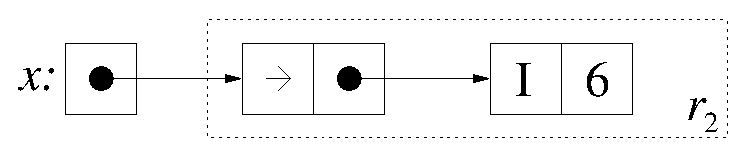
\includegraphics[scale=0.5]{2-System/fig/class-lazy-indir}
\end{center}

During back end code generation, we must account for the fact that $x$ may point to a thunk or indirection. To extract the unboxed integer from $x$ we must first load the tag of the object pointed to. This allows us to identify the sort of object it is, and decide whether to force the thunk, follow the indirection, or load the value as required. On the other hand, if we knew that $x$ was direct, as with:

\code{
	$x$	& $::$ 	& $\iInt \ r_2' \ \rhd \ \iDirect \ r_2'$ \\
}

Then we would be sure that $x$ only pointed to a boxed integer. This would save us from having to load the tag and do the test. Similarly to the way non-mutable regions default to being constant, non-lazy regions default to being direct.

\subsection{Liftedness is not a capability}
\label{System:Effects:liftedness}

We should note that the constraint names $\iLazy$ and $\iDirect$ have an operational flavour because DDC uses this information to guide optimisations. We could perhaps rename them to $\iLifted$ and $\iUnlifted$, which would reflect the fact that a $\iLifted$ value represents a computation that may diverge. 

A similar approach is taken in \cite{launchbury:unboxing-unpointed-types} and \cite{peyton-jones:bridging-the-gulf}, though they distinguish between pointed and lifted types. In \cite{launchbury:unboxing-unpointed-types}, the type of unlifted integers is written $\iInt^{\#}$. The type of lifted integers is defined to be $\iInt^{\#}_{\bot}$, with the $\bot$ in the subscript acting as a type operator that allows the bottom element to be one of the ``values'' represented by the type. Note that with this formulation, monotypes such as integers must be either lifted or unlifted. 

Our method of attaching constraints to region variables allows us to reuse the type class machinery to encode a similar property. However, type class constraints express a ``supports'' relationship, which doesn't quite match up with the concept of liftedness. For example, the constraint $\iEq \ a$ means that $a$ is a type whose values support being tested for equality. The constraint $\iMutable \ r$ means that the objects in region $r$ support being updated. Likewise, $\iConst \ r$ means that the objects in $r$ can be safely read by a suspended computation, that is, they support laziness. If an object is constrained to be neither $\iMutable$ nor $\iConst$ then we cannot assume it is safe to do either of these things. 

Extensionally, if a type is completely unconstrained then we know nothing about the values that inhabit that type. Each new constraint provides a new piece of information, and that information gives us the capability to do something new with the corresponding values.

If a region is $\iDirect$ then we can generate faster code to read objects in that region, because they are guaranteed not to be represented by thunks. However, the fact that a region is $\iLazy$ doesn't provide us with an additional capability. $\iLazy$ constraints are used only to ensure that a region is not also treated as $\iDirect$, as once we add thunks to a region we must test for them when reading every object from that region. In this sense, $\iLazy$ is a sort of ``anti-capability'' that indicates that a region has definitely been polluted by thunks and can no longer be used ``directly''.

For example, consider the following type:

\code{
	$\ifun :: \forall r_1 \ r_2. \ \iInt \ r_1 \to \iInt \ r_2$
}

As $r_1$ is unconstrained, objects passed to this function \emph{may} be represented by thunks. If instead we had:

\code{
	$\ifun :: \forall r_1 \ r_2. \ \iInt \ r_1 \to \iInt \ r_2 \ \rhd \ \iDirect \ r_1$
}

Then objects passed to the function are guaranteed \emph{not} to be represented by thunks, and we can optimise the function using this information. On the other hand, if we had:

\code{
	$\ifun :: \forall r_1 \ r_2. \ \iInt \ r_1 \to \iInt \ r_2 \ \rhd \ \iLazy \ r_1$
}

The $\iLazy$ constraint says that objects passed to this function may be represented by thunks, but this isn't new information compared with the first version. However, during type inference, if we discover that a term has type:

\code{
	$\iInt \ r_1 \rhd \iLazy \ r_1, \ \iDirect \ r_1$
}

Then this could mean that a lazy object, which might be a thunk, was passed to a function that can only accept a direct object, which cannot be a thunk. This is invalid, and will be marked as a type error.



\clearpage{}
% -------------------------
\section{The problem with polymorphic update}

\label{System:PolyUpdate}
A well known problem can arise when destructive update is added to a language with a Hindley-Milner style polymorphic type system. The classic example is as follows:

\code{	$\iid$ 	& $:: \forall a. \ a \to a$ 	\\
	$\isucc$	& $:: \iInt \to \iInt$	 	
}

\code{	\mc{2}{$\ibroken \ ()$} \\
	\ $= \kdo$ 	& $\iref = \inewRef \ \iid$		\\
			& $\iwriteRef \ \iref  \ \isucc$	\\
	 		& $(\ireadRef \ \iref) \ \iTrue$	\\
}


If we treated this function as though it were written in Standard ML, we could argue that it is not type safe and would likely crash at runtime. The first line creates a reference to a polymorphic function $\iid$, while the second updates it to hold a less general function $\isucc$. This invalidates the original type of $\iref$. The problem appears to center on the type inferred for $\iref$:

\code{
	$\iref :: \forall a. \ \iRef \ (a \to a)$
}

The $\forall$-quantifier allows us to instantiate this type differently for each use of $\iref$. However, our static type system is unable to track the fact that once we update the reference we can no longer treat it has having this general type.

% --------------------
\subsection{Fighting the value restriction}
After winning out over several other systems \cite{garrigue:relaxing} the standard way of addressing the problem with polymorphic update is to apply the \emph{value restriction} \cite{wright:polymorphism-imperative}. The value restriction states that the type of a let-bound variable should only be generalised if the right of the binding is a syntactic value, such as a variable, literal, lambda abstraction, or application of a data constructor to another value. These expressions are called \emph{non-expansive} because their evaluation will neither generate an exception or extend the domain of the store \cite{milner:sml, tofte:polymorphic-references}. 

The value restriction has the advantages that it is simple, easy to implement, and does not require extra information to be attached to the structure of types. This last point is especially important for ML-style languages in which the programmer must write full type signatures when defining module interfaces.

The down side is that a class of expressions that were previously assigned polymorphic types lose their polymorphism. For example:

\code{
	$f = \imap \ \iid$
}

The type of $f$ is not generalised because the right of the binding is not a syntactic value. To regain polymorphism we must $\eta$-expand it to give:

\code{
	$f = \lambda x. \ \imap \ \iid \ x$
}

or equivalently, write it as a function binding:

\code{
	$f \ x = \imap \ \iid \ x$
}

In \cite{wright:polymorphism-imperative} it was argued that as the number of modifications needing to be performed to existing ML programs was small compared to the overall size of the code, the value restriction does not place an undue burden on the programmer in practice. However, in light of more recent languages such as Haskell \cite{haskell98-report}, the value restriction would interfere with applications such as parser combinator libraries, which make heavy use of polymorphic values \cite{leigen:parsec}.

More recently, a variant named the \emph{relaxed value restriction} \cite{garrigue:relaxing} uses a subtyping based approach to recover some of the polymorphism lost by the simpler restriction. Unfortunately,  straight-forward examples like $(\imap \ \iid)$ remain monomorphic.


% --------------------
\subsection{Don't generalise variables free in the store typing}
\label{System:PolyUpdate:dontgeneralise}
In \cite{tofte:polymorphic-references} Tofte uncovers the crux of the problem with polymorphic update by attempting to prove the soundness of an ML-style type system with mutable references, and showing where the proof breaks down.

Unsurprisingly, the offending case is the one for let-bindings. The dynamic rule is as follows:

\ruleBox{
	\begin{gather}
	\ruleI
	{MLEvLet}
	{ s \s E \vdash t_1 \longrightarrow v_1 \s s_1 \qq
	  s_1 \s E + \{x \mapsto v_1\} \ \vdash t_2 \longrightarrow v \s s' }
	{ s \s E \vdash \textbf{let} \ x = t_1 \ \textbf{in} \ t_2 \longrightarrow v \s s'}
	\end{gather}
}

\medskip
The judgement form $s \s E \vdash t \longrightarrow v \s s'$ is read: starting with store $s$ and environment $E$, the expression $t$ evaluates to value $v$ and a (perhaps changed) store $s'$. The store $s$ maps locations to values while the environment $E$ maps variables to values. Store locations are created when we allocate a new reference cell, and modifying the contents of a reference cell corresponds to changing the value bound to a particular location. The corresponding type rule is:

\ruleBox{
	\begin{gather}
	\ruleI
	{MLTyLet}
	{ \Gamma \vdash t_1 :: \tau_1 \qq
          \Gamma, \ x : \textrm{Gen}(\Gamma, \ \tau_1) \vdash t_2 :: \tau }
	{ \Gamma \vdash \textbf{let} \ x = t_1 \ \textbf{in} \ t_2 :: \tau }
	\end{gather}
}

\medskip
Here, $\textrm{Gen}(\Gamma, \ \tau_1)$ performs generalisation and is short for $\forall a_1 .. a_n. \ \tau_1$, where $a_1 ...  a_n$ are the type variables in $\tau_1$ that are not free in $\Gamma$. 

In general, $t_1$ may contain location variables, so we need to know the types of the values bound to these locations before we can check the type of the whole expression. This information is held in the \emph{store typing} which maps locations to types. 

If we have an expression $t_1$ of type $\tau_1$, then reducing it relative to a particular store $s_1$ should yield a value $v_1$. We desire this value to have the same type as the original expression, and express this fact with the statement:

\code{
	$s_1 :: ST_1 \models v_1 :: \tau_1$
}

This statement reads: in store $s_1$ with typing $ST_1$, $v_1$ has type $\tau_1$. Now the trouble starts. Although we know that $v_1$ has type $\tau_1$, when evaluating a let-expression we must satisfy the the second premise of (MLTyLet). 

\clearpage{}
This requires that we strengthen the previous statement to:

\code{
	$s_1 :: ST_1 \models v_1 :: \textrm{Gen}(\Gamma, \ \tau_1)$
}

This says that we're now considering the value to have a more general type than it used to. An example of this would be to first treat the term $(\lambda x. \ x)$ as having the monomorphic type $b \to b$, and then later deciding that it has the more general, polymorphic type \ $\forall b. \ b \to b$. In a language without references, as long as $b$ is not free in the type environment then this generalisation is justified. 

If $b$ is not free in the type environment, then there is nothing stopping us from $\alpha$-converting any local uses of it, and thus eliminating all mention of this particular variable from our typing statements. By doing this we could be sure that no other parts of the program are treating $b$ as being any specific, concrete type, because they have no information about it.

However, when we introduce mutable references we must also introduce the concept of a store and its associated store typing. This store typing includes type variables, and when we try to strengthen the original statement the proof falls apart. Consider again our $\ibroken$ example that creates a reference to the polymorphic function $\iid$. Expanding out the definition of $\iid$ gives:

\code{
	$\klet \ \iref = \inewRef \ (\lambda x. \ x)$	 \\
	$\kin \ \ \dots$
}

Once $\inewRef \ (\lambda x. \ x)$ has been reduced to a value, the statement we need to strengthen is:

\code{
	$\{ \iloc_1 \mapsto \lambda x. \ x \} :: \{ \iloc_1 \mapsto (a \to a) \}
	\ \models \ loc_1 :: a \to a$
}

Notice how the reduction of $\inewRef \ (\lambda x. \ x)$ has created a new location in the store and bound the identity function to it. In the \emph{store typing} this function has the type $(a \rightarrow a)$ which includes the free variable $a$. 

However, during generalisation this fact is ignored and we end up with:

\code{
	$\{ \iloc_1 \mapsto \lambda x. \ x \} :: \{ \iloc_1 \mapsto (a \rightarrow a) \}
	\ \models \ loc_1 :: \mbox{\boldmath $\forall a. \ a \rightarrow a$}$
}

This statement is clearly suspect because the type assigned to $\iloc_1$ no longer models its type in the store. When we update the reference to hold $\isucc$, the type of the binding in the store changes. Unfortunately, the static typing rules still treat $\iloc_1$ as having the more general type:

\code{
	$\{ \iloc_1 \mapsto \isucc \} :: \{ loc_1 \mapsto (\iInt \to \iInt) \}
	\ \models \ \iloc_1 :: \mbox{\boldmath $\forall a. \ a \rightarrow a$}$
}

If we were to then read the $\isucc$ function back from the store and apply it to a non-$\iInt$ value like $\iTrue$, the runtime result would be undefined.

Tofte sums up the problem with the following observation:
\begin{center}
\begin{minipage}{30em}
\emph{The naive extension of the polymorphic type discipline} [with mutable references] \emph{fails because
it admits generalisation on type variables that occur free in the store typing.}
\end{minipage}
\end{center}


\subsection{Generalisation reduces data sharing in System-F}
\label{System:PolyUpdate:Sharing}
The value restriction does not solve the fundamental problem of a static analysis being unable to track runtime changes in the type of data. What it does is to limit polymorphism, and to prevent the user from writing a certain class of programs.

Issues of \emph{soundness} can only arise in relation to a well defined semantics. The usual formulation being ``Soundness = Progress + Preservation'' \cite{pierce:tapl}, meaning that a well-typed expression must either be a value or be able to progress to the next step in its evaluation; and that its well-typing is preserved during evaluation.

With an ML style semantics, if we fail to deal adequately with the issue of polymorphic update then the last line in $\ibroken$ from \S\ref{System:PolyUpdate} reduces as:

\code{
  	\mc{2}{$(\ireadRef \iref) \ \iTrue$}		\\
	& $\lfun \ \isucc \ \iTrue$			\\
 	& $\lfun \ (\lambda x. \ x + 1) \ \iTrue$ 	\\
 	& $\lfun \ \iTrue + 1$
}

This term is not a value and cannot be evaluated further as there is no reduction rule specifying how to add one to a boolean value. It is the \emph{combination} of operational and static semantics which is unsound.

On the other hand, if we consider a System-F style translation of $\ibroken$ which has been typed without restricting generalisation then we would have:
\begin{displaymath}
\begin{split}
\ibroken & = \lambda \ (). \\
   & \klet \ \iref \ 	    = \Lambda b. \ \inewRef \ \{b \to b\} \ (\iid \ \{b\}) \ \ \kin \\
   & \klet \ \_  \ \ \ \ \: = \iwriteRef \ \{ \iInt \rightarrow \iInt \} \ (\iref \ \{\iInt \}) \ \isucc \ \ \kin \\
   & \ireadRef \ \{ \iBool \to \iBool\} \ (\iref \ \{ \iBool \}) \ \iTrue \\
\end{split}
\end{displaymath}

We have inserted type lambdas $\Lambda$ and type arguments \texttt{\{\}} at generalisation and instantiation points respectively. Notice that $\iref$ now binds a \emph{function value} instead of an application expression. 

From the operational semantics of DDC's core language \S\ref{Core:Simplified:Transitions} we have:

\ruleBox{
	\begin{gather}
	\ruleI	{EvLet1}
		{ \heap  \with t_1 \eto
		  \heap' \with t_1' 
		}
		{ \heap  \with \rblet \ x = t_1  \ \rbin \ t_2 \eto
		  \heap' \with \rblet \ x = t_1' \ \rbin \ t_2 
		}
	\ruleSkip
	\ruleA	{EvLet}
		{ \heap  \with \rblet \ x = v^\circ \ \rbin \ t \eto
		  \heap  \with t[v^\circ/x] 
		}
	\end{gather}	
}

When combined, these two rules say that to evaluate a let-expression we should first reduce the right of the binding to a (weak) value and then substitute this value into the body. While evaluating $\ibroken$, as the right of the $\iref$ binding is already a value we substitute and end up with:
\begin{displaymath}
\begin{split}
   & \klet \ \_  \ \ \ \  
   	= \iwriteRef \ \{ \iInt \to \iInt \} 
		\ ((\Lambda b. \ \inewRef \ \textbf{...} )\ \{\iInt \}) \ \isucc \ \ \kin \\
   &  \ireadRef \ \{\iBool \to \iBool\} \ ((\Lambda b. \ \inewRef \ \textbf{...} ) \ \{\iBool\}) \ \iTrue \\
\end{split}
\end{displaymath}

Note the duplication of the term involving $\inewRef$ and the fact that a new reference containing $\iid$ will be allocated at each occurrence. The re-evaluation of polymorphic terms corresponds with \emph{polymorphism-by-name}~\cite{leroy:polymorphism-by-name}. Also note that the first reference will be updated, but only the second one will be read. Admittedly, the behavior of this expression could be confusing to the programmer, but allowing it does not make our system unsound. Demonstration of unsoundness would require that an expression was well typed, not a value, and could not be reduced further. This expression can be reduced to $\iTrue$, and is not a problem in this respect.

Although polymorphism-by-name keeps our System-F style \emph{core} language sound in the presence of polymorphic update, we expect it to be too confusing for the programmer to use in practice. If a value appears to be shared in the source program, then we do not want this sharing to be reduced depending on whether it is assigned a polymorphic type by the type inferencer. As in \cite{gifford:integrating} we restrict generalisation to preserve the data sharing properties of programs during translation to and from core. However, as mentioned earlier we don't want to use the value restriction. The next section discusses the possibility of leveraging effect typing to control generalisation, but as we shall see in \S\ref{System:Closure} we use another method, namely \emph{closure typing}, to achieve this. Closure typing will help us deal with the problem with polymorphic update, as well as more accurately reason about the sharing properties of data.


% --------------------
\subsection{Restricting generalisation with effect typing}
As we don't want to rely on the value restriction to control generalisation, we must find another way of identifying variables that are free in the store typing. In a language with ML-style references, the sole means of extending the store is by explicitly allocating them with a function such as $\inewRef$. In this case, the problem of identifying variables free in the store typing reduces to identifying calls to $\inewRef$ and collecting the types of values passed to it. If we treat reference allocation as a computational effect, then we can use effect inference to perform the collection \cite{wright:references-effect}. The rules for the polymorphic type and effect system \cite{talpin:polymorphic, talpin:discipline} are as follows:

\vspace{-1em}
\begin{displaymath}
\tfbox{\Gamma \judge t \hastype \tau \with \sigma}
\end{displaymath}
\ruleBox{
	\begin{gather*}
	\ruleA	{Var}
		{\Gamma, \ x : \tau &
			\judge x
			\hastype \textrm{Inst}(\tau)
			\with \emptyset} 
	\ruleSkip
	\ruleI	{Abs}
		{ \Gamma, \ x : \tau_1 &
			\judge t_2
			\hastype \tau_2
			\with \sigma }
		{ \Gamma &
			\judge \lambda (x : \tau_1). \ t_2 	
			\hastype \tau_1 \funa{\sigma} \tau_2
			\with \emptyset}
	\ruleSkip
	\ruleI	{App}
		{ \Gamma & 
			\judge t_1 
			\hastype \tau_{11} \funa{\sigma} \tau_{12}
			\with \sigma_1  \\
	  	\Gamma & 
			\judge t_2 			
			\hastype \tau_{11}
			\with \sigma_2 \\ }
		{ \Gamma & 
			\judge t_1 \ t_2
			\hastype \tau_{12}
			\with \sigma_1 \cup \sigma_2 \cup \sigma }
	\ruleSkip
	\ruleI	{Let}
		{ \Gamma &
			\judge t_1
			\hastype \tau_1
			\with \sigma_1 \\
	  	\Gamma, \ x : \textrm{Gen}(\sigma_1, \Gamma, \tau_1) & 
		  	\judge t_2
			\hastype \tau_2
			\with \sigma_2 \\ }
		{ \Gamma
			\judge \textbf{let} \ x = t_1 \ \textbf{in} \ t_2
			\hastype \tau_2
			\with \sigma_1 \cup \sigma_2 }
	\ruleSkip
	\ruleI	{Sub}
		{ \Gamma & \judge t \hastype \tau \with \sigma_1 \tspace \sigma_1 \subseteq \sigma_2}
		{ \Gamma & \judge t \hastype \tau \with \sigma_2 }
	\end{gather*}
}


 
The judgement \ $\Gamma \judge e \hastype \tau \with \sigma$ \ reads: In the environment $\Gamma$ the expression $e$ has type $\tau$ and effect $\sigma$. The environment $\Gamma$ maps variables to types. In this presentation effects are gathered together with the set union operator $\cup$ and a pure expression is assigned the effect $\emptyset$. Also note the term $\textrm{Gen}(\sigma_1, \Gamma, \tau_1)$ in the rule (Let). Generalisation is restricted to variables that are not free in either the type environment or the effect caused by evaluating the body of a let-binding.

These rules describe the ``plumbing'' of how effects are attached to types. What's missing is a description of how atomic effects are introduced to the system via $\inewRef$.

In Wright's system \cite{wright:references-effect}, $\inewRef$ is given the type:

\code{
	$\inewRef :: \forall a \ e. \ a \lfuna{a \ e} \iRef a$
}

Here, $a$ is a type variable and its presence on the function arrow indicates that it has the effect of allocating a new reference containing a value of that type. The effect variable $e$ combined with the subsumption rule (Sub) allows the function to be treated as causing \emph{any} effect so long as it includes $a$. This is used when passing arguments to higher order functions, which is discussed in \S\ref{System:Effects:constraint-strengthening}. Although this system collects the requisite type variables, it is limited by the fact that \emph{all} the effects caused by the allocation of references appear in a function's type, even if they are used entirely locally to that function. 

For example, with the following program:

\code{
	$\iid$		& $ :: \forall a \ e. \ a \funa{e} a$ \\
	$\iid$		& $ = \lambda x. \ x$ 
	\\[1ex]
	$\iidRef$	& $:: b \funa{b} b$ \\
	$\iidRef$ 	& $= (\lambda x. \ \klet \ \iref = \inewRef \  x \ \kin \ \ireadRef \ \iref)$
}

In the type for $\iid$, we can generalise $a$ because it does not appear free in either the type environment or the effect caused by the function. The second function $\iidRef$ behaves identically to $\iid$, except that it creates a reference to its argument before returning it. Even though this reference is not accessible once $\iidRef$ returns, the effect caused by allocating it appears in its type, which prevents $b$ from being generalised. Although these two functions behave identically from a \emph{callers} point of view, they cannot be used interchangeably as they have different types.



% --------------------
\subsection{Observation criteria}
\label{System:PolyUpdate:observation}
In \cite{talpin:discipline} Talpin and Jouvelot extend Wright's effect system with regions. As in Disciple, their regions denote sets of locations which may alias, but they attach region variables to reference types only. In their system, effects are caused when references are read and written to, but also when they are allocated. Each effect carries with it the type of the reference being acted upon, as well as the region it is contained within. The types of the primitive operators are:
% -- Type schemes

\code{
	$\inewRef $
	& $::$	& $\forall a \ r \ e. \ (a \lfuna{e} \iRef \ r \ a)$
	 	  $\rhd \ e \supseteq \iInit \ r \ a$
	\\[1ex]
	$\ireadRef$ 
	& $::$	& $\forall a \ r \ e.	\ (\iRef \ r \ a \lfuna{e} a)$
	 	  $\rhd \ e \supseteq \iRead \ r \ a$
	\\[1ex]
	$\iwriteRef$ 
	& $::$	& $\forall a \ r \ e. \ (\iRef \ r \ a \lfuna{e_1} a \lfuna{e_2} ())$
	 	  $\ \rhd \ e_2 \supseteq \iWrite \ r \ a$
}

\medskip
Similarly to Wright's system, $\inewRef$ can be treated has having \emph{any} effect, so long as that effect includes $\iInit \ r \ a$. The effect $\iInit \ r \ a$ records that a reference in region $r$ was initialised to contain a value of type $a$. However, in this system the subsumption rule (Sub) is modified to include an observation criterion which allows effects which are not visible to a caller to be masked.

% -- sub-obs
\ruleBox{
	\begin{gather*}
	\ruleI	{Sub-Obs}
		{ \Gamma & \judge e \hastype \tau \with \sigma_1 
			\tspace \sigma_2 \supseteq \iObserve(\Gamma, \sigma_1, \tau)}
		{ \Gamma & \judge e \hastype \tau \with \sigma_2 }
	\end{gather*}
}

where

\code{
	\mc{2}{$\iObserve(\Gamma, \tau, e)$} 
	\\[1ex]
 	& $= \{ \ \iInit \ r \ \tau_1, \ \iRead \ r \ \tau_1, \ \iWrite \ r \ \tau_1 \in \sigma \ 
 			| \ r \in \ifr(\Gamma) \cup \ifr(\tau) \ \}$ 
	\\[1ex]
 	& $\cup \ \{ \ \varsigma \in \sigma \ | \ \varsigma \in \ifv(\Gamma) \cup fv(\tau) \ \}$
}

The function $\ifv$ computes the free type, region and effect variables in its argument, while $\ifr$ returns free region variables only.

With this system, when we type check the definition of $\iidRef$ the body of the $\lambda$-expression yields the statement:

\code{
	$\Gamma, \ x :: a$ 
		& $\judge (\klet \ \iref = \inewRef \ x \ \kin \ \ireadRef \ r) :: a$ \\
		& $\ ; \ \iInit \ r_1 \ a \ \cup \ \iRead \ r_1 \ a$
}

Note that although the right of the let-binding allocates and then reads a reference, the region into which the reference is allocated is entirely local to the binding. Applying (Sub-Obs) yields:

\code{
	$\Gamma, \ x :: a$
		& $\judge (\klet \ \iref = \inewRef \ x \ \kin \ \ireadRef \ r) :: a$ \\
		& $\ ; \ \emptyset$
}

This allows us to infer the same type for $\iid$ as we do for $\iidRef$. Leaving the formal proof of soundness in \cite{talpin:discipline}, we can see why the observation criteria works by inspecting our original statement:

\code{
	$\Gamma, \ x :: a$ 
		& $\judge (\klet \ \iref = \inewRef \ x \ \kin \ \ireadRef \ r) :: a$ \\
		& $\ ; \ \iInit \ r_1 \ a \ \cup \ \iRead \ r_1 \ a$
}

Notice that $r_1$ is not present in the type environment, and is therefore not visible to the expression's calling context. Also, as the type of the expression does include $r_1$ there will be no ``handle'' on this region after the expression has finished evaluating. Indeed, as the allocated reference is unreachable after this evaluation, it could be safely garbage collected. Returning to Tofte's (un)proof in \S\ref{System:PolyUpdate:dontgeneralise}, this garbage collection corresponds to removing the associated binding from the store and its store typing, which allows $a$ to be safely generalised.


% --------------------
\subsection{Effect typing versus arbitrary update}
Talpin and Jouvelot's system works well for a language with ML-style references. As update is limited to a distinguished $\iRef$ type, it is easy for the type system to decide when to introduce $\iRead$, $\iWrite$ and $\iInit$ effects. However, in Disciple, update is not restricted to data of a special type. In our system all data has the potential to be updated. 

\clearpage{}
For example the simple data type $\iMaybe$ is defined as follows:

\code{
	$\kdata \ \iMaybe \ r \ a \ = \iNothing \ | \ \iJust \ a$
}

Defining this type furnishes us with a data constructor which can be used to allocate a $\iJust$.

\code{
	$\iJust :: \forall \ a \ r. \ a \to \iMaybe \ r \ a$
}

Once a $\iJust$ has been allocated, we can then use the field projection syntax of \S\ref{System:Projections} to update it, or not, as we see fit. If we were to use an effect system to control generalisation, how would we know whether this constructor should cause an $\iInit$ effect? Only the allocation of a mutable value should cause an effect, but mutability depends on whether or not the value may ever be updated, not \emph{vice versa}. The mutability of the object will be inferred by our type system, but this property is not immediately visible at the point where the object is allocated.


% --------------------

% \subsection{Value versus monomorphism restrictions in Haskell}
% Although Haskell does not suffer problems with polymorphic update, there is a related problem involving data sharing. This problem also involves the conversion of pattern bindings to function bindings and is addressed by the infamous monomorphism restriction \cite{haskell98-report}.

% \begin{itemize}
% \item	Adding dictionary parameters to values changes them into functions. 
%	This reduces sharing which can cause performance problems.
%\item	It is important not to reduce sharing of mutable data. Doing so can cause the meaning 
%	of the program to change. If the body of a loop updates a mutable value at an outer scope, 
%	and we shift it into the body, then successive iterations of the loop cannot see results
%	from the previous ones.
% \item	Haskell doesn't suffer problems with polymorphic update because the translation of monadic bindings
%	does not use let, so there is no generalisation.
% \end{itemize}


\clearpage{}
\section{Closure typing}
\label{System:Closure}

Leroy's \emph{closure-typing} \cite{leroy:polymorphic-type-inference, leroy:polymorphic-typing} is a system for modeling data sharing due to the inclusion of free variables in the bodies of functions. 
We use closure typing as an alternate solution to the problem of polymorphic update, as well as to reason about the sharing properties of regions. 

Consider the following function:

\code{
	$\iaddT = \lambda x. \ \lambda y. \ (x + y, \ x)$
}

If we take addition $(+)$ to operate on values of type $\iInt$, then we could give $\iaddT$ the following type:

\code{
	$\iaddT :: \iInt \to \iInt \to \iPair \ \iInt \ \iInt$
}

If we then partially apply $\iaddT$ to the value 5, the first argument of its type is satisfied and we end up with a function that accepts an integer and produces a pair:

\code{
	$\iaddFive :: \iInt \to \iPair \ \iInt \ \iInt$ \\
	$\iaddFive = \iaddT \ 5$ \\
}

$\iaddFive$ can be further applied to yield the pair, but what happened to the first value we provided? Assume  evaluation proceeds via template instantiation after the pure lambda calculus. In this case we could reason that the argument $5$ was bound to the formal parameter $x$ and then substituted into the body of the outer lambda abstraction, that is:

\code{
	$\iaddFive$ 
	& $\longrightarrow \iaddT \ 5$	\\
	& $\longrightarrow (\lambda x. \ \lambda y. \ ( x + y, \ x)) \ 5$ \\
	& $\longrightarrow \lambda y. \ (5 + y, \ 5)$ 
}

This call-by-name reasoning is applicable to a pure language such as Haskell, but as we intend to use
destructive update we must take a more operational approach. If we instead consider an implementation based on super-combinators \cite{hughes:thesis}, we would treat $\iaddT$ as a single supercombinator, and the partial application $(\iaddT \ 5)$ as the construction of a thunk containing pointers to the supercombinator code and argument value:

\begin{center}
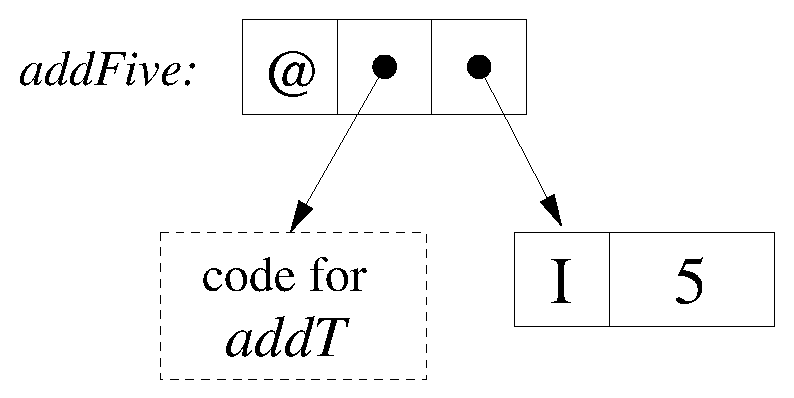
\includegraphics[scale=0.4]{2-System/fig/closure-super.eps}
\end{center}

When $\iaddFive$ is applied to its final argument, the code for $\iaddT$ is called directly. $\iaddT$'s first argument comes from the thunk, and the second is supplied by the application. This is how DDC operates.

With this system, every use of $\iaddFive$ shares the same `5' object. Using region annotations on data types and closure annotations on functions\footnote{We modify Leroy's syntax for closures to be similar to the one used for effects.}, we give $\iaddFive$ a type which makes the sharing explicit.

\code{
	$\iaddFive$ 
	& $::$		& $\forall r_1 \ r_2 \ r_3$ \\
	& $.$		& $\iInt \ r_1 \lfuna{c_1} \iPair \ r_2 \ (\iInt \ r_3) \ (\iInt \ r_4)$ \\
      	& $\rhd$	& $c_1 = x : \iInt \ r_4$ \\
}

On the left of the function arrow, the argument type $\iInt \ r_1$ says that $\iaddFive$ accepts an integer from a region which we name $r_1$. On the right of the arrow, we see that the function produces a pair of integer components. As $r_3$ is quantified, we infer that the first component has been freshly allocated into a new region (addition returns a fresh result). The data constructor representing the pair is also fresh, so $r_2$ is quantified as well. On the other hand, $r_4$ is \emph{not} quantified, which indicates that the second component of the pair will be in the same region each time $\iaddFive$ is called. 

The closure variable $c_1$ attached to the function arrow indicates that the definition of $\iaddFive$ creates a shared value, and the term $x : \iInt \ r_4$ records its type. The ``$x :$'' portion of $x : \iInt \ r_4$ is called the \emph{closure tag}, and we treat it as an operator that lifts the type term $\iInt \ r_4$ into a closure term. In this example, the variable $x$ corresponds to the occurrence that is free in the innermost lambda-abstraction in the definition of $\iaddFive$. For the types of primitive functions such as data constructors, although there is no associated source code we still use names such as $x, y, z$ for consistency. 

Note that our type system tracks variable names such as $x$ as a notational convenience, but does not make use of them for checking purposes. We have found it useful for such variables to be included in the types presented to the user, as without them it can be very difficult to determine why an inferred type signature includes a particular closure term. However, if desired we could replace all such variables with an underscore to indicate they are ignored by the type system proper.

% --------------------
\subsection{Dangerous type variables}
\label{System:Closure:dangerous}

In \cite{leroy:polymorphic-typing} Leroy defines dangerous variables to be the ones that are free in a live reference type. For Disciple this is equivalent to being free under a mutable type constructor.

Consider the following type:

\code{
	$\ithing$	
	& $::$		& $\iMaybe \ r_1 \ (a \to a)$ \\
	& $\rhd$	& $\iMutable \ r_1$
}

\quad with

\code{
	\mc{4}{$\kdata \ \iMaybe \ r_1 \ a$} \\
		& $=$	& $\iNothing$ \\
		& \ $|$	& $\iJust \ \{ x :: a \}$
}

In the type of $\ithing$, $a$ is dangerous because it corresponds to a value that we are able to update at runtime. For example, the following code creates a $\iJust$ constructor containing the function $\iid$, updates it to hold the less general function $\isucc$, then tries to apply that function to a string. This example is similar to one from \S\ref{System:PolyUpdate}, except that we are using the Disciple projection syntax to update the mutable object. The term $\ithing \ \odot_{\#} \ x$ creates a reference to the $x$ field in the $\iJust$ constructor. If we view references as being akin to pointers, then $\ithing \ \odot_{\#} \ x$ has a similar meaning to the C expression \texttt{\&(thing.x)}. Projections are discussed further in \S\ref{System:Projections}. 

\clearpage{}
Once the reference is created, we use the $:=_{\#}$ operator to update the field (via the reference):

\code{ 
	$\kdo$	& $\ithing$	& $= \iJust \ \iid$ 
		\\[1ex]
		& $thing \ \odot_{\#} \: x$	
				& ${:=_{\#}} \ \isucc$ 
		\\[1ex]
		& $\itrouble$	& $= \kcase \ \ithing \ \kof \ {\iJust \ f \to \ f \ ``\texttt{die!}"}$
}

When generalising the type of $\ithing$ we must hold $a$ monomorphic. If we were to give it the following polymorphic type, then the above code would pass the type checker, but would have an undefined result at runtime.

\code{
	$\ithing_{\ibad}$	
	& $::$		& $\forall a. \ \iMaybe \ r_1 \ (a \to a)$ \\
	& $\rhd$	& $\iMutable \ r_1$
}

In general, to determine the dangerous variables in a type we must inspect the definitions of the data types involved. 

For example, the following type has three separate region variables, which gives us three places to attach mutability constraints:

\code{
	\mc{3}{$\kdata \ \iTwoThings \ r_1 \ r_2 \ r_3 \ a \ b$} \\
	& $=$	& $\iThingOne \ (\iMaybe \ r_2 \ a)$ \\
	& $\ |$	& $\iThingTwo \ (\iMaybe \ r_3 \ b)$
}

Here is an example signature that uses $\iTwoThings$:

\code{
	$\ifoo$	& :: 		& \mc{3}{$\iTwoThings \ r_4 \ r_5 \ r_6 \ (d \to \iInt \ r_7) \ (\iChar \ r_8)$} \\
		& $\rhd$	& $\iConst \ r_4$	\\
		& , 		& $\iMutable \ r_5$	\\
		& ,		& $\iConst \ r_6$
}

In this case, as $r_5$ is mutable we must hold $d$ and $r_7$ monomorphic. Note that region, effect and closure variables can be dangerous as well. As $r_5$ is mutable we cannot generalise $r_7$ because the associated $\iMaybe$ object might be updated to hold a function that does not allocate a fresh return value. On the other hand, we can allow $r_8$ to be polymorphic as $r_6$ is constant. If $r_4$ was mutable then all of $r_5$, $r_6$, $d$, $r_7$ and $r_8$ would have to be monomorphic, because this would let us update either of the $\iThing$ objects to hold a different $\iMaybe$.

A formal description of which variables are dangerous is given in \S\ref{Inference:Language}.


% ----------------
\subsection{Closure typing and hidden communication}
\label{System:Closure:masking}

Consider the following function, also from \cite{leroy:polymorphic-typing}:

\code{
	\mc{4}{$\imakeGetSet \ x$} \\
	& $\kdo$	& $\iref$	& $= \inewRef \ x$ \\
	&		& $\iget \ ()$	& $= \ireadRef \ \iref$ \\
	&		& $\iset \ z$	& $= \iwriteRef \ \iref \ z$ \\
	&		& \mc{2}{$\iPair \ \iget \ \iset$}
}

This function allocates a reference to the supplied value $x$, and then returns a pair of functions to get and set the value in the reference. 

\clearpage{}
In Disciple, without closure information and before generalisation, the type of $\imakeGetSet$ is:

\code{
	$\imakeGetSet$ 
	& $::$		& \mc{2}{$a \to \iPair \ r_1 \ (() \lfuna{e_1} a) \ (a \lfuna{e_2} ())$} \\
	& $\rhd$	& $e_1$		& $\tme \iRead \  r_2$ \\
	& $,$		& $e_2$		& $\tme \iWrite \ r_2$ \\
	& $,$		& \mc{2}{$\iMutable \ r_2$}
}

There are two problems with this type. Firstly, as $r_2$ is not mentioned in the body (or the type environment), the read and write effects will be masked as per \S\ref{System:Effects:masking}. This is invalid because the order in which these applications take place at runtime certainly matters, so they must retain their effect terms. Secondly, if we were to allow $a$ to be generalised then we would have an unsound system once again. 

For example:

\code{
	$\imakeGetSet_{\ibad}$ 
	& $::$		
	& \mc{2}{$\forall a \ r_1. \ a \to \iPair \ r_1 \ (() \to a) \ (a \to ())$} \\
}

\code{
	\mc{4}{$\ibroken \ ()$} \\
	& $\kdo$	& $\igetset$	& $= \imakeGetSet_{\ibad} \ \iid$ 
	\\[1ex]
	&		& $\isetTwo$	& $= \isnd \ \igetset$ \\
	&		& \mc{2}{$\isetTwo \ \isucc$}
	\\[1ex]
	&		& $\igetTwo$	& $= \ifst \ \igetset$ \\
	&		& \mc{2}{$\igetTwo \ () \ ``\texttt{die!}"$}
}


By allowing the mutable object $\iref$ to be free in the closure of the get and set functions, we have created a communication channel between them that is not visible in their types. This is not a problem in itself, but the addition of let-polymorphism allows each function to gain a different understanding of what type of data is being sent across the channel. Note that with the bad type for $\imakeGetSet$, the inferred type of $\igetset$ includes a quantifier for $b$:

\code{
	$\igetset$	:: $\forall b. \ \iPair \ r_1 \ (() \to (b \to b)) \ ((b \to b) \to ())$ \\
}

As we have used a let-binding to define $\igetTwo$ and $\isetTwo$, the types of the two components are re-generalised and we end up with:

\code{
	$\igetTwo$	:: $\forall c. \ () \to (c \to c)$ \\
	$\isetTwo$	:: $\forall d. \ (d \to d) \to ()$ \\
}

The use of $\isetTwo$ updates the shared reference to contain a function, $\isucc$, that only accepts integers. Unfortunately, with $\igetTwo$ we can then read it back and pretend that it accepts a string.

Adding closure information to our types remedies this problem. Here is the new type of $\imakeGetSet$, with closure information, and before generalisation:

\code{
	$\imakeGetSet$ 
	& $::$		& \mc{2}{$a \to \iPair \ r_1 \ (() \lfuna{e_1 \ c_1} a) \ (a \lfuna{e_2 \ c_2} ())$} \\
	& $\rhd$	& $e_1$		& $\tme \ \iRead \  r_2$ \\
	& $,$		& $e_2$		& $\tme \ \iWrite \ r_2$ \\
	& $,$		& $c_1$		& $\tme \ \iref : \iRef \ r_2 \ a$ \\
	& $,$		& $c_2$		& $\tme \ \iref : \iRef \ r_2 \ a$ \\
	& $,$		& \mc{2}{$\iMutable \ r_2$}
}

The constraints on $c_1$ and $c_2$ show that the get and set functions returned in the pair can access a shared mutable value, and that the type of this value contains a variable $a$. Note that the lattice structure for closures is identical to that for effects, which was discussed in \S\ref{System:Effects:interference}. For closures we take $\tme$ as being a synonym for the superset operator $\supseteq$, and use $\lor$ as a synonym for $\cup$. There is no $\top$ element for closures, but we stick with the lattice notation for consistency with effect types.

Returning to $\imakeGetSet$, note that this function allocates the reference itself. This can be determined from the fact that the primary region variable of the reference, $r_2$, is not reachable from the closure annotation on the outermost (leftmost) function arrow. Once we apply $\imakeGetSet$ to its argument, the reference is created and subsequently shared. In our example this is done in the binding for $\igetset$.

After generalisation, the new type of $\igetset$ is:

\code{
	$\igetset$
	& $::$		& \mc{2}{$\forall e_1 \ e_2 \ c_1 \ c_2$} \\
	& $.$		& \mc{2}{$\iPair \ r_1 \ (() \lfuna{e_1 \ c_1} (b \to b)) \ 
					((b \to b) \lfuna{e_2 \ c_2} ())$} \\
	& $\rhd$	& $e_1$		& $\tme \ \iRead \  r_2$ \\
	& $,$		& $e_2$		& $\tme \ \iWrite \ r_2$ \\
	& $,$		& $c_1$		& $\tme \ \iref : \iRef \ r_2 \ (b \to b)$ \\
	& $,$		& $c_2$		& $\tme \ \iref : \iRef \ r_2 \ (b \to b)$ \\
	& $,$		& \mc{2}{$\iMutable \ r_2$}
}

In this type we have two ``outermost" function arrows, which are the two in the $\iPair$. The type $(b \to b)$ is in the closure of these outermost functions, and the type variable $b$ lies underneath a region variable $r_2$ that is constrained to be $\iMutable$. This means that $b$ is dangerous and cannot be generalised. Note that $r_2$ is not generalised either, though this restriction is due to the fact that $r_2$ is present in the outermost closure. This point is discussed in the next section.

Returning to our example, after performing the $\ifst$ and $\isnd$ projections, our new types for $\igetTwo$ and $\isetTwo$ are:

\code{
	$\igetTwo$	
	& $::$		& \mc{2}{$\forall e_1 \ c_1. \ () \lfuna{e_1 \ c_1} (b \to b)$} \\
	& $\rhd$	& $e_1$		& $\tme \ \iRead \ r_2$ \\
	& $,$		& $c_1$		& $\tme \ \iref : \iRef \ r_2 \ (b \to b)$ \\
	& $,$		& \mc{2}{$\iMutable \ r_2$}
	\\[1em]
	$\isetTwo$	
	& $::$		& \mc{2}{$\forall e_2 \ c_2. \ (b \to b) \lfuna{e_2 \ c_2} ()$} \\
	& $\rhd$	& $e_2$		& $\tme \ \iWrite \ r_2$ \\
	& $,$		& $c_2$		& $\tme \ \iref : \iRef \ r_2 \ (b \to b)$ \\
	& $,$		& \mc{2}{$\iMutable \ r_2$}
}

The effect information in the types of these functions ensures that uses of them will not be reordered during optimisation. The closure annotations capture the fact that they can communicate via a shared mutable value, and ensures that both functions agree on its type.

\clearpage{}
% --------------------
\subsection{Material regions and sharing}
\label{System:Closure:shared-regions}

Recall from section \S\ref{System:Regions:non-material} that \emph{material} region variables are the ones that represent objects that are shared between all uses of a bound variable. For example:

\code{
	$\ifive :: \iInt \ r$	\\
	$\ifive = 5$		
}

Here, $r$ is clearly material, because every use of $\ifive$ references the same `5' object. On the other hand, consider:

\code{
	\mc{2}{$\iaddTwo :: \forall r_1 \ r_2. \ \iInt \ r_1 \to \iInt \ r_2$} \\
	$\iaddTwo \ x$	& $= \isucc \ (\isucc \ x)$
}

Neither $r_1$ or $r_2$ are material in the type of $\iaddTwo$. These variables represent the locations of objects passed to, and returned from, the function. They do not represent locations of objects that are shared between uses of it. Without further information, we take regions in the argument positions of function types to be immaterial. 

Note that with the constructors at hand, we cannot be sure that no \emph{function objects} are shared between calls to $\iaddTwo$. If $\isucc$ was defined as the partial application of some more primitive function, then every use of $\isucc$ would refer to the same thunk. However, for our purposes sharing only matters if the shared objected has the potential to be destructively updated, and thunks cannot be updated.\footnote{They can be overwritten by the runtime system during lazy evaluation, but this is not visible in the programming model.} 

The following example defines a function that references a shared data object:

\code{
	\mc{2}{$\imakeFive \ ()$} \\
	\ $= \kdo$
		& $x$			& $= 5$ \\
		& $\iretFive \ ()$	& $= x$ \\
		& $\iretFive$
}

If we wrote down a type for $\imakeFive$ which included region variables but not closure information then we would have:

\code{
	$\imakeFive :: \forall r. \ () \to () \to \iInt \ r$
}

As $r$ is quantified, $\imakeFive$ should return a freshly allocated $\iInt$ object each time it is called. This is certainly true if we apply both arguments, but we can invalidate the meaning of the quantifier by supplying only one. To see this more clearly, consider the supercombinator translation:

\code{
	\mc{2}{$\imakeFive' \ ()$} \\
	\ $= \kdo$
		& $x$	& $= 5$	\\ 
		& \mc{2}{$\iretFive' \ x$}
}

\vspace{-1ex}
\code{	
	$\iretFive' \ x' \ ()$	& $= x'$ \\
}

$\imakeFive'$ and $\iretFive'$ are the result of lambda-lifting \cite{johnsson:lambda-lifting} our original function. Note that the free variable in the definition of $\iretFive$ is passed explicitly to its lifted version. As $\imakeFive'$ returns the value $\iretFive' \ x$, which evaluates to a thunk, the same `$5$' object will be returned each time $\imakeFive'$ is provided with its final argument. 

Consider then a binding that partially applies $\imakeFive$:

\code{
	$\imakeFiveUnit :: \forall r. \ () \to \iInt \ r$ \\
	$\imakeFiveUnit = \imakeFive \ ()$
}

Although the type of $\imakeFiveUnit$ says that its return value should be freshly allocated, we have just seen that the evaluation of  $\imakeFive \ ()$ will produce a function that returns the same `5' object every time. Following the standard restriction for generalisation, we have not quantified over variables free in the type environment. This environment consists of the type of $\imakeFive$, which has no free variables, so that does not help us here. The standard restriction prevents types from becoming out of sync with their context, but it does not model sharing due to free variables in the body of function definitions.

Once again, closure typing comes to our rescue. When we include closure information, the types of $\imakeFive$ and $\imakeFiveUnit$ become:

\code{
	$\imakeFive$ 	
		& $::$		& $\forall r. \ () \to () \funa{c} \iInt \ r$ \\
	 	& $\rhd$ 	& $c = x : \iInt \ r$ 
	\\[1ex]
	
	$\imakeFiveUnit$
		& $::$ 		& $() \funa{c} \iInt \ r$ \\
		& $\rhd$	& $c = x : \iInt \ r$ \\
}

The type of $\imakeFive$ now includes the fact that when the first $()$ is applied, it allocates an object in a region it names $r$, and this object is shared by all calls to the returned function.

The type of $\imakeFiveUnit$ preserves this sharing information. Region variables that are reachable from the closure annotation on the outer most function arrow of a type are material, and material region variables are not generalised.


% --------------------
\subsection{Material regions and algebraic data types}
\label{System:Closure:non-material-regions}

When we come to generalise the type of a binding, and the type contains only simple constructors like $\iInt$ and $\fun$, then we can determine which region variables are material directly from the type. However, when dealing with algebraic data types, we also need their definitions.

Consider the following:

\code{
	\mc{4}{$\kdata \ \iIntFun \ r_{1..4} \ e_1 \ c_1$} \\
	& $=$	& $\iSInt$ $(\iInt \ r_2)$ \\
	& $|$	& $\iSFun$ $(\iInt \ r_3 \lfuna{e_1 \ c_1} \iInt \ r_4)$ 
}

This definition implicitly generates the following constructors. Note that we use $r_1..r_4.$ as shorthand for $r_1 \ r_2 \ r_3 \ r_4.$ Also, $r_1$ is used as the primary region variable of the type, but is not present in the types of the constructor arguments.

\code{
	$\iSInt$ 
	& $::$	& $\forall r_{1..4} \ e_1 \ c_1$ \\
	& $.$	& $\iInt \ r_2 \fun \iIntFun \ r_{1..4} \ e_1 \ c_1$ 
	\\[1ex]
	$\iSFun$
	& $::$	& $\forall r_{1..4} \ e_1 \ c_1$ \\
	& $.$	& $(\iInt \ r_3 \lfuna{e_1 \ c_1} \iInt \ r_4) \to \iIntFun \ r_{1..4} \ e_1 \ c_1$
}

The $\iSInt$ constructor creates an object containing a pointer to an $\iInt$. The region variable $r_1$ is primary as it is first in the list, so we take the outer $\iSInt$ constructor to be in this region. The $\iInt$ component is in region $r_2$, so an application of $\iSInt$ would produce:

\code{
	& \qq \qq $\isomeFive$	& $= \iSInt \ 5$ \\
}

\vspace{-1em}
\begin{center}
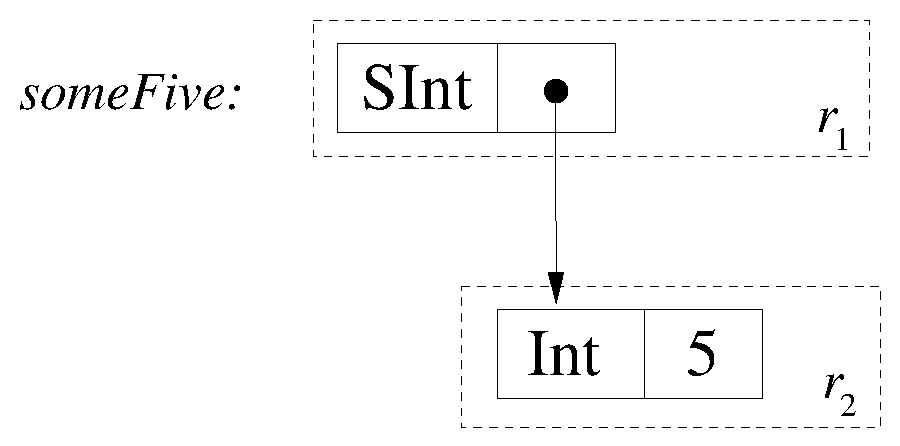
\includegraphics[scale=0.4]{2-System/fig/closure-someFive.eps}
\end{center}

As the outer constructor always appears in the primary region, the primary region variable is material. Because an $\iSInt$ object contains an $\iInt$ in a region named $r_2$, this variable is also material.

On the other hand, when we use $\iSFun$, the constructed object will contain a pointer to either the code for the function argument, or a thunk, depending on whether the argument was partially applied:

\begin{tabbing}
 	MMMMM \= MMMMMMMMMMM \= MMMMM \= MMMMMMMM \kill
	$\isomeSucc$ \> $= \iSFun \ \isucc$  \> $\isomeAdd$ \> $= \iSFun \ ((+) \ 2)$
\end{tabbing}

\vspace{-2em}
\begin{center}
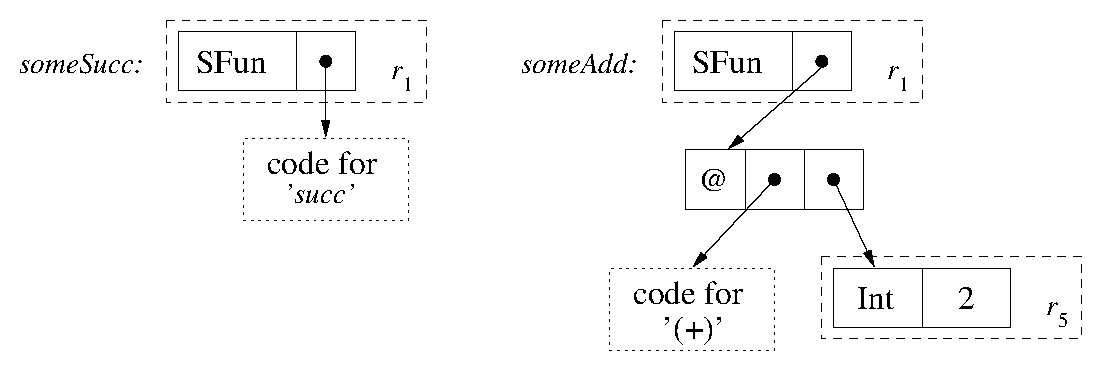
\includegraphics[scale=0.7]{2-System/fig/closure-someSuccAdd.eps}
\end{center}

Note that with the constructors at hand, there no way to create an $\iIntFun$ object that actually includes data in the $r_3$ or $r_4$ regions. Because of this, they are immaterial, and the generalisation of immaterial regions is not restricted as per the previous section. The type of $\isomeSucc$ above is:

\code{
	$\isomeSucc $
	& $::$		& \mc{3}{$\forall r_3 \ r_4 \ e_1. \ \iIntFun \ r_{1..4} \ e_1 \ \bot$} \\
	& $\rhd$ 	& $e_1$	& $\tme \iRead \ r_3$
}

Note that although our $\isomeSucc$ object does not include data in region $r_2$, that region is not quantified here. In general, if a particular value has type $\iIntFun \ r_{1..4} \ e_1 \ c_1$ then we will not know what data constructor was used to create it. We must rely on the data type definition to determine which regions are material.

The type of $\isomeAdd$ is similar, except that its closure variable is constrained to contain the type of the argument in the partial application of $(+)$:

\code{
	$\isomeAdd$ 
	& $::$		& \mc{2}{$\forall r_3 \ r_4 \ e_1 \ c_1. \ \iIntFun \ r_{1..4} \ e_1 \ c_1$} \\
	& $\rhd$	& $e_1$		& $\tme \iRead \ r_3 \lor \iRead \ r_5$ \\
	& $,$		& $c_1$		& $\tme \iInt \ r_5$
}

The material regions of a type are defined formally in \S\ref{inference:material-regions}.

\clearpage{}
% -----------------
\subsection{Strong, mixed and absent region variables}
\label{System:Closure:strong-mixed-absent-variables}

When an algebraic data type is defined we do not restrict the ways in which region variables are used. Due to this, a particular variable may occur in both a material and immaterial position. For example:

\code{
	\mc{4}{$\kdata \ \iIntFunMixed \ r_{1..5} \ e_1 \ c_1$} \\
	& $=$	& $\iSIntX$	& $(\iInt \ r_2)$ \\
	& $|$	& $\iSCharX$	& $(\iInt \ r_4)$ \\
	& $|$	& $\iSFunX$	& $(\iInt \ r_2 \lfuna{e_1 \ c_1} \iInt \ r_3)$
}

In the first constructor, $r_2$ is used as the primary region variable of $\iInt$, which makes it material. In the third constructor, $r_2$ is used as part of the type of a function parameter, so it is also immaterial. In this situation we say that $r_2$ is \emph{mixed material}.

If a region variable is \emph{only} ever used in a material position, then it is \emph{strongly material}. In the above definition, $r_1$ is strongly material because it is used as the primary region variable for $\iIntFunMixed$, and not in the type of a function parameter. The variable $r_4$ is also strongly material. We will use this concept when we discuss the polymorphic copy function in \S\ref{System:TypeClassing}. 

If a region variable is present as a parameter of the type constructor being defined, but not one of the data constructors, then we say it is \emph{absent}. The variable $r_5$ is absent in the above definition. As absent region variables cannot correspond to real regions in the store, all absent variables are also immaterial. The reverse is not true, as $r_3$ is immaterial, but not absent.


% --------------------
\subsection{Pure effects and empty closures}
\label{System:Closure:empty}
In the previous two sections, the definitions of $\iIntFun$ and $\iIntFunMixed$ include effect and closure variables as arguments to the type constructor. This allows these data types to be polymorphic in the effect and closure of the contained function. Alternatively, we could omit these variables as long as we constrained the types of $\iSFun$ and $\iSFunX$ so that the effect of the contained function was pure, and its closure contained no elements. 

A closure that has no elements is said to be \emph{empty}. Emptiness of closures is related to purity of effects. Recall from \S\ref{System:Effects:purification} that a pure effect is written $\bot$ and we can require an effect to be pure with the $\iPure$ constraint. Likewise, we write empty closures as $\bot$ and require a closure to be empty with the $\iEmpty$ constraint. We sometimes annotate $\bot$ with its kind, such as $\bot_{!}$ and $\bot_{\$}$ to distinguish between its two readings, but the kind is usually clear from context.

By omitting effect and closure variables, and restricting ourselves to a single region we will now define a diet version of $\iIntFun$ that has a single parameter instead of six. This new data type can still contain an $\iInt$ or function value, but the set of functions it could hold is reduced:

\code{
	\mc{4}{$\kdata \ \iIntFunDiet \ r_1$} \\
	& $=$	& $\iSIntD$	& $(\iInt \ r_1)$ \\
	& $|$	& $\iSFunD$	& $(\iInt \ r_1 \to \iInt \ r_1)$
}

\clearpage{}
\code{
	\mc{4}{$\kdata \ \iIntFunDiet \ r_1$} \\
	& $=$	& $\iSIntD$	& $(\iInt \ r_1)$ \\
	& $|$	& $\iSFunD$	& $(\iInt \ r_1 \to \iInt \ r_1)$
}

This modified data type definition generates the following constructors:

\code{
	$\iSIntD$ 
		& $::$ 	& $\forall r_1. \ \iInt \ r_1 \to \iIntFunDiet \ r_1$ 
	\\[1em]
	$\iSFunD$ 
		& $::$		& $\forall r_1 \ e_1 \ c_1$ \\
		& $.$	& $(\iInt \ r_1 \lfuna{e_1 \ c_1} \iInt \ r_1) \to \iIntFunDiet \ r_1$ \\
		& $\rhd $		& $\iPure \ e_1$ \\
		& $, $		& $\iEmpty \ c_1$ \\
}

Note that although $r_1$ is repeated in the first parameter of $\iSFunD$, this doesn't require its argument to be a function which simply passes the $\iInt$ through unchanged. The type of a function like $\isucc$ can be instantiated so that both its region variables are the same. Due to this we can still construct $(\iSFunD \ \isucc)$ as per the figure in \S\ref{System:Closure:non-material-regions}, though the single region will be forced $\iConst$ due to purification of the function's $\iRead$ effect. On the other hand, we can no longer construct $(\iSFunD \ ((+) \ 2))$ as its type would include a closure term due to the partial application, rendering it non-empty. See \S\ref{Evaluation:Limits:sharing-and-constraint-masking}
 for a possible way of addressing this limitation.

% --------------------
% \subsection{Shared regions which escape the analysis}
% Although closure typing goes a long way to model data sharing, inspection of the figures in the previous sections shows us that not all such data in the program is visible to the type system. In particular, the thunk created due to the partial application of $(+)$ in figure \ref{fig:typeSystem:uses-of-sfun} has not been assigned a region. 

% This is an important difference between our use of region variables and the way they are used in system such as MLKit\cite{tofte:mlkit-4.3.0}. In MLKit, \emph{all} data is assigned to a particular region, including thunks, which implies that function types are given region annotations as well \cite{tofte:region-inference}. In that system, regions are used for memory management whereas in ours they are used to identify non-interfering sets of computational effects, and to reason about mutability of data.

% \begin{itemize}
% \item	The lifetimes of thunks does not follow procedure activation closely. This is mentioned in MLKit paper about
% 	combining GC with region allocation.
% \item	We don't have region vars on function types, so we can't allocate them in regions, but we expect this not
% 	to be a problem.
% \item	Reference that paper on imperative data structures and the \texttt{close} operator.
% \end{itemize}


% --------------------
\subsection{Closure trimming}
\label{System:Closure:trimming}

The closure annotation attached to a function type lists the types of all free variables in that function's definition. However, not all of this information is useful to our analysis. As we only restrict the generalisation of material region variables, we only need to retain closure terms that contain them. The rest of the closure information can be trimmed out, and doing so is an important optimisation in practice.

Consider the following program:

\code{
	$x$ 		& 	& $= 5$			\\
 	$\ifun$		& ()  	& $= x + 1$ 		\\
 	$\ifunTwo$	& () 	& $= \ifun$  		\\
 	$\ifunThree$	& () 	& $= \ifunTwo$		\\
	$\ifunFour$	& () 	& $= \ifunThree$
}

This is a simple program, but as each successive binding refers to the binding above it, the closure terms in their types can become very large.

If $x$ has type $\iInt \ r_1$, then $\ifun$ has the following signature:

\code{
	$\ifun$ 
	& $::$		& $\forall r_2. \ () \lfuna{e_1 \ c_1} \iInt \ r_2$ \\
	& $\rhd$	& $e_1 = \iRead \ r_1$ \\
	& $,$		& $c_1 = x : \iInt \ r_1$
}

This says that $\ifun$ accepts a unit value and produces a freshly allocated integer. The closure constraint $c_1 = x : \iInt \ r_1$ says that the function refers to this object via the free variable $x$. When it evaluates, the addition operator reads the integer bound to $x$, hence the $\iRead \ r_1$ effect. It also reads the constant integer $1$, but as this constant is local to the function the effect is masked. 

\clearpage{}
Here is the type for $\ifunTwo:$

\qq\qq
\begin{tabular}{llllllll}
	$\ifunTwo$
	& $::$	& \mc{5}{$\forall r_2. \ () \lfuna{c_2} () \lfuna{e_1 \ c_1} \iInt \ r_2$} \\
	& $\rhd$& $e_1$	& \mc{3}{$= \iRead \ r_1$}	\\
	& $,$	& $c_1$	& \mc{3}{$= x : \iInt \ r_1$} 	\\
	& $,$	& $c_2$	& $= (\ifun$ 	& $:$	& \mc{2}{$\forall r_3. \ () \lfuna{e_3 \ c_3} \iInt \ r_3$} \\
	&	&	& 		& $\rhd$	& $e_3$		& $= \iRead \ r_1$ \\
	&	&	&	 	& $,$		& $c_3$		& $= x : \iInt \ r_1)$
\end{tabular}
\medskip

Note that $\ifunTwo$ refers to $\ifun$, so the full type of $\ifun$ appears in its closure. However, as we only use closure terms to reason about the sharing properties of data, we gain no benefit from carrying around information about the effects associated with a variable like $\ifun$. We also gain no benefit from retaining its argument and return types. We extend the concept of materiality to value types, and say that the argument and return positions of functions are immaterial because they do not represent objects in the store. Lastly, if we erase the return type $\iInt \ r_3$ then we do not need the quantifier $\forall r_3$. The only information about $\ifun$ that we \emph{do} need to keep is that it references a material object of type $\iInt \ r_1$. Using these observations we trim the type of $\ifunTwo$ to get:


\qq\qq
\begin{tabular}{llllllll}
	$\ifunTwo$
	& $::$	& \mc{5}{$\forall r_2. \ () \lfuna{c_2} () \lfuna{e_1 \ c_1} \iInt \ r_2$} \\
	& $\rhd$& $e_1$	& \mc{3}{$= \iRead \ r_1$}	\\
	& $,$	& $c_1$	& \mc{3}{$= x : \iInt \ r_1$} 	\\
	& $,$	& $c_2$	& $= \ifun : \iInt \ r_1$ 
\end{tabular}

Trimming closures prevents the types of functions from ``blowing up''. Without closure trimming the closure term of a top level function like $\imain$ would include all the types of all functions used in the program. In practice, most closure terms can be erased totally. For example, the definition of our $\iaddTwo$ function references the free variable $\isucc$. As $\isucc$ contains no material closure components, neither does $\iaddTwo$.

\code{
	\mc{2}{$\iaddTwo :: \forall r_1 \ r_2. \ \iInt \ r_1 \to \iInt \ r_2$} \\
	$\iaddTwo \ x$	& $= \isucc \ (\isucc \ x)$
}

In our current implementation we only trim out closure information concerning \emph{immaterial} region variables. Section \S\ref{Evaluation:Limits:sharing-and-constraint-masking} presents some ideas for also trimming out information concerning region variables that are constrained to be constant.



\clearpage{}
\section{Type classing}
\label{System:TypeClassing}
In this section we discuss value type classes in Disciple. The general mechanism is similar to that used in Haskell, except that we need a special $\iShape$ constraint on types to be able to write useful class declarations.

As our current implementation does not implement dictionary passing, we limit ourselves to situations where the overloading can be resolved at compile time. For this reason, none of our class declarations have superclasses, and we do not support value type classes being present in the constraint list of a type. This in turn allows us to avoid considering most of the subtle issues discussed in \cite{peyton-jones:type-class-design-space}. We have made this restriction because we are primarily interested in using the type class mechanism to manage our region, effect and closure information. Exploring the possibilities for interaction between the various kinds of constraints represents an interesting opportunity for future work. There is also the possibility of defining multi-parameter type classes that constrain types of varying kinds. 


% -------------------------------------
\subsection{Copy and counting}
The need for a $\iShape$ constraint arises naturally when we consider functions that copy data. For example, the  $\icopyInt$ function which copies an integer value has type:

\code{
	$\icopyInt$ 
		& $::$	 & $\forall r_1 \ r_2. \ \iInt \ r_1 \lfuna{e_1} \ \iInt \ r_2$ \\
		& $\rhd$ & $e_1 = \iRead \ r_1$
}

We will assume that this function is defined as a primitive. As $r_2$ is quantified we know that $\icopyInt$ allocates the object being returned, which is what we expect from a copy function.

In Disciple programs, $\icopyInt$ can be used to initialise mutable counters. For example:

\code{
	\mc{3}{$\istartValue :: \iInt \ r_1 \rhd \iConst \ r_1$} \\
	\mc{3}{$\istartValue = 5$}
\\[1em]
	$\ifun \ ()$ \\
	\ = $\kdo$	& $\icount$	& $= \icopyInt \istartValue$ \\
			& $\dots$ \\
			& $\icount$	& $:= \icount - 1$ \\
			& \dots
}

$\istartValue$ is defined at top level. In Disciple, if a top level value is not explicitly constrained to be $\iMutable$ then $\iConst$ constraints are added automatically. We have included this one manually for the sake of example.

In the definition $\ifun$ we have a counter that is destructively decremented as the function evaluates. As the type of $(:=)$ (sugar for $\iupdateInt$) requires its argument to be mutable, we cannot simply initialise the counter with the binding $\icount = \istartValue$. This would make the variable $\icount$ an alias for the object bound to $\istartValue$. This in turn would require both $\icount$ and $\istartValue$ to have the same type, creating a conflict between the mutability constraint on $\icount$ and the constancy constraint on $\istartValue$. We instead use $\icopyInt$ to make a fresh copy of $\istartValue$, and this use object to initialise $\icount$. 



% -------------------------------------
\subsection{Type classes for copy and update}
\label{System:TypeClassing:copy-and-update}

After integers, another common data type in functional programs is the list. In Disciple we can declare the list type as:

\code{
	\mc{3}{$\kdata \ \iList \ r_1 \ a$} \\
	& $=$		& $\iNil$ \\
	& $\ \mid$ 	& $\iCons \ a \ (\iList \ r_1 \ a)$
}

This declaration introduces the data constructors $\iNil$ and $\iCons$ which have the following types:

\code{
	$\iNil$		& $:: \forall r_1 \ a. \ \iList \ r_1 \ a$ 
	\\[1ex]
	$\iCons$	& $:: \forall r_1 \ a. \ a \to \iList \ r_1 \ a 
					\lfuna{c_1} \iList \ r_1 \ a$ \\
			& $\rhd \ c_1 = x : a$
}

Note that in the type of $\iNil$, the region variable $r_1$ is quantified. This indicates that $\iNil$ behaves as though it allocates a fresh object at each occurrence.\footnote{However, if the returned object is constrained to be constant then the compiler can reuse the same one each time and avoid the actual allocation.} On the other hand, in the type of $\iCons$ the region variable $r_1$ is shared between the second argument and the return type. This indicates that the returned object will contain a reference to this argument.

Using our list constructors, and the $\icopyInt$ function from the previous section, we define $\icopyListInt$ which copies a list of integers:

\code{
	$\icopyListInt$
	& $::$	 	& $\forall r_1 \ r_2 \ r_3 \ r_4$ \\
	& $.$ 		& $\iList \ r_1 \ (\iInt \ r_2) \lfuna{e_1} \ \iList \ r_3 \ (\iInt \ r_4)$ \\
	& $\rhd$ 	& $e_1 = \iRead \ r_1 \lor \iRead \ r_2$
}

\code{
	\mc{2}{$\icopyListInt \ xx$} \\
		& $= \kcase \ xx \ \kof$ \\
		& \qq $\iNil$		& $\to \iNil$ \\
		& \qq $\iCons x \ xs$	& $\to \iCons \ (\icopyInt \ x) \ (\icopyListInt \ xs)$ 
}

Once again, the fact that both $r_3$ and $r_4$ are quantified indicates that the returned object is freshly allocated. Note that $e_1$ includes an effect $\iRead \ r_1$ due to inspecting the spine of the list, as well as $\iRead \ r_2$ from copying its elements.

As $\icopyInt$ and $\icopyListInt$ perform similar operations, we would like define a type class that abstracts them. If we ignore effect information for the moment, we could try something like:

\code{
	\mc{4}{$\kclass \ \iCopy \ a \ \kwhere$} \\
	& $\icopy$	& $::$	&$a \to a$
}

Unfortunately, this signature for $\icopy$ does not respect the fact that the returned object should be fresh. Our $\icopyInt$ function produces a freshly allocated object, but $\iInt$ instance of the type in the class declaration would be:

\code{
	$\icopy_{\iInt}$ 
		& $::$	 & $\forall r_1. \ \iInt \ r_1 \to \ \iInt \ r_1$ \\
}

This would prevent us from using our overloaded $\icopy$ function to make local, mutable copies of constant integers as per the previous section. As the argument and return types include the same region variable, any constraints placed on one must be compatible with the other. On the other hand, the following class declaration is too weak:

\code{
	\mc{4}{$\kclass \ \iCopy \ a \ \kwhere$} \\
	& $\icopy$	& $::$	& $\forall b. \ a \to b$
}

If the argument of $\icopy$ is an integer, then we expect the return value to also be an integer. What we need is for the argument and return types of $\icopy$ to have the same overall \emph{shape}, while allowing their contained region variables to vary. 

We enforce this with the $\iShape$ constraint:

\code{
	\mc{4}{$\kclass \ \iCopy \ a \ \kwhere$} \\
	& $\icopy$ 	& $::$		& $\forall b. \ a \to b$ \\
	&		& $\rhd$	& $\iShape \ a \ b$
}

$\iShape \ a \ b$ can be viewed as functional dependency \cite{jones:functional-dependencies} between the two types $a$ and $b$. The functional dependency is bi-directional, so if $a$ is an $\iInt$ then $b$ must also be an $\iInt$, and if $b$ is an $\iInt$ then so must $a$. As we do not provide any mechanism for defining $\iShape$ from a more primitive structure, it is baked into the language. 

This handles the argument and return types, though we still need to account for the effect of reading the argument. We do this with the $\iReadT$ (read type) effect:

\code{
	\mc{4}{$\kclass \ \iCopy \ a \ \kwhere$} \\
	& $\icopy$ 	& $::$		& $\forall b. \ a \lfuna{e_1} b$ \\
	&		& $\rhd$	& $e_1 = \iReadT \ a$ \\
	&		& $, $		& $\iShape \ a \ b$
}

In the class declaration, $\iReadT \ a$ says that instances of the $\icopy$ function are permitted to read any region variable present in the type $a$. Once this declaration is in place, we can add the instances for each of our copy functions:

\code{
	\mc{4}{$\kinstance \ \iCopy \ (\iInt \ r_1) \ \kwhere$} \\
	& $\icopy$	& $= \icopyInt$ 
	\\[2ex]
	\mc{4}{$\kinstance \ \iCopy \ (\iList \ r_1 \ (\iInt \ r_2)) \ \kwhere$} \\
	& $\icopy$ 	& $= \icopyListInt$
}

Along with $\iReadT$, there is a related $\iWriteT$ that allows a function to have a write effect on any region variable in a type. Similarly, $\iMutableT$ and $\iConstT$ place constraints on all the region variables in a type. 

Next, we will use $\iWriteT$ and $\iMutableT$ to define the type class of objects that can be destructively updated:

\code{
	\mc{4}{$\kclass \ \iUpdate \ a \ \kwhere$} \\
	& $(:=)$	& $::$		& $\forall b. \ a \to b \lfuna{c_1 \ e_1} ()$ \\
	&		& $\rhd$	& $e_1 = \iWriteT \ a \ \lor \ \iReadT \ b$ \\
	&		& $, $		& $c_1 = x : a$ \\
	&		& $, $		& $\iShape \ a \ b$ \\
	&		& $, $		& $\iMutableT \ a$ \\
}

This declaration says that instances of $(:=)$ may write to the first argument, read the second argument, hold a reference to the first argument during partial application, require both arguments to have the same overall shape, and require regions in the first argument to be mutable.

Note that the types in class declarations are \emph{upper bounds} of the possible types of the instances. Instances of $(:=)$ must have a type which is at least as polymorphic as the one in the class declaration, and may not have an effect that is not implied by $\iWriteT \ a \ \lor \ \iReadT \ b$. Nor may they place constraints on their arguments other than $\iShape \ a \ b$ and $\iMutableT \ a$. Importantly, after a partial application of just their first arguments, they may not hold references to any material values other than these arguments. This last point is determined by the closure term $x : a$.


% -------------------------------------
\subsection{Shape and partial application}
\label{System:TypeClassing:shape-and-partial-application}

We now discuss how the $\iShape$ constraint works during partial application. We will use the overloaded equality function as an example. Here is the $\iEq$ class declaration:

\code{
	\mc{4}{$\kclass \ \iEq \ a \ \kwhere$} \\
	& $(==)$	& $::$		& $\forall b \ r_1. \ a \to b \lfuna{e_1 \ c_1} \iBool \ r_1$ \\
	&		& $\rhd$	& $e_1 = \iReadT \ a \ \lor \ \iReadT \ b$ \\
	&		& $,$		& $c_1 = x : a$ \\
	&		& $,$		& $\iShape \ a \ b$
}

This declaration says that instances of $(==)$ accept two arguments, and return a fresh boolean. Instances are permitted to read their arguments and hold a reference to the first one when partially applied. The arguments may also be required to have the same shape.

Consider the following binding:

\code{
	$\iisEmpty$	& $=$	& $(==)\  [\ ]$
}

This binding partially applies $(==)$, resulting in a function that tests whether a list is empty. To determine the type of $\iisEmpty$ we first instantiate the type of $(==)$:

\code{
	$(==)$ \quad \	
		& $::$		& $a' \to b' \lfuna{e_1 \ c_1} \iBool \ r_1'$ \\
		& $\rhd$	& $e_1 = \iReadT \ a' \ \lor \ \iReadT\ b'$ \\
		& ,		& $c_1 = x : a'$ \\
		& ,		& $\iShape \ a' \ b'$
}

Taking $[ \ ]$ to have the type $\iList \ r_2 \ c$, we bind it to $a'$ and eliminate the outer function constructor:

\code{
	$((==) \ [\ ])$ 
		& $::$		& $b' \lfuna{e_1 \ c_1} \iBool \ r_1'$ \\
		& $\rhd$	& $e_1 = \iReadT \ (\iList \ r_2 \ c) \ \lor \ \iReadT\ b'$ \\
		& ,		& $c_1 = x : \iList \ r_2 \ c$ \\
		& ,		& \mc{2}{$\iShape \ (\iList \ r_2 \ c) \ b'$}
}

The $\iShape \ (\iList \ r_2 \ c) \ b'$ constraint requires $b'$ to have the same shape as $\iList \ r_2 \ c$. We satisfy this by giving $b$ the type $\iList \ r_3 \ d$, where $r_3$ and $d$ are fresh:

\code{
	$((==) \ [\ ])$ 
		& $::$		& $\iList \ r_3 \ d \lfuna{e_1 \ c_1} \iBool \ r_1'$ \\
		& $\rhd$	& $e_1 = \iReadT \ (\iList \ r_2 \ c) \ \lor \ \iReadT \ (\iList \ r_3 \ d)$ \\
		& ,		& $c_1 = x : \iList \ r_2 \ c$ \\
		& ,		& \mc{2}{$\iShape \ (\iList \ r_2 \ c) \ (\iList \ r_3 \ d)$}
}

The effect $\iReadT$ expresses a read on all region variables in its argument type. As we now know what this argument type is we can reduce the $\iReadT$ effect to a simpler form. Here, $\iReadT \ (\iList \ r_2 \ c)$ can be reduced to $\iRead \ r_2 \lor \iReadT \ c$ and $\iReadT \ (\iList \ r_3 \ d)$ can be reduced to $\iRead \ r_3 \lor \iReadT \ d$. As both arguments to our $\iShape$ constraint are list types, this constraint is partially satisfied, though we still need to ensure that $c$ has the same shape as $d$:

\code{
	$((==) \ [\ ])$ 
		& $::$		& $\iList \ r_3 \ d \lfuna{e_1 \ c_1} \iBool \ r_1'$ \\
		& $\rhd$	& $e_1 = \iRead \ r_2 \lor \iReadT \ c \lor \iRead \ r_3 \lor \iReadT \ d$ \\
		& ,		& $c_1 = x : \iList \ r_2 \ c$ \\
		& ,		& \mc{2}{$\iShape \ c \ d$}
}

This type can be reduced no further, so we will generalise it to create the scheme for $\iisEmpty$:

\code{
	$\iisEmpty$ 
		& $::$		& $\forall c \ d \ r_1 \ r_3$ \\
		& . 		& $\iList \ r_3 \ d \lfuna{e_1 \ c_1} \iBool \ r_1$ \\
		& $\rhd$	& $e_1 = \iRead \ r_2 \lor \iReadT \ c \lor \iRead \ r_3 \lor \iReadT \ d$ \\
		& ,		& $c_1 = x : \iList \ r_2 \ c$ \\
		& ,		& \mc{2}{$\iShape \ c \ d$}
}

Note that as per \S\ref{System:Closure:shared-regions} we have not generalised $r_2$ because it appears in the outermost closure of the function. At runtime, the application of $(==)$ to $[\ ]$ will build a thunk containing a pointer to the function and the empty list. This empty list is shared between all uses of $\iisEmpty$.


% -------------------------------------
\subsection{Shape constraints and rigid type variables}
Consider the following Haskell type class declaration:

\code{
	\mc{4}{$\kclass \ \iFoo \ a \ \kwhere$} \\
	& $\ifoo$	& $::$	& $\forall b. \ a \to [b] \to [b]$
}

An instance of this class is:

\code{
	\mc{4}{$\kinstance \ \iFoo \ Bool \ \kwhere$} \\
	& $\ifoo \ x \ y$	& $= \kif \ x \ \kthen \ \itail \ y \ \kelse \ \ireverse \ y$
}

The locally quantified type variable $b$ is called a \emph{rigid type variable}. This highlights the fact that every instance of $\ifoo$ must have a similarly general type. For example, the following instance is invalid:

\code{
	\mc{4}{$\kinstance \ \iFoo \ \iChar \ \kwhere$} \\
		& $\ifoo \ x \ y = \kif \ x  == `a` \ \kthen \ \itail \ y \ \kelse \ [x]$
}

This non-instance tries to assign $\ifoo$ the following type:

\code{
	\mc{4}{$\ifoo_{\iChar} :: \iChar \to [\iChar] \to [\iChar]$}
}

This is strictly less general than the one in the type class declaration, because we cannot apply it to lists whose elements do not have type $\iChar$. 

The $\iCopy$ type class declaration also contains a rigid type variable. Here it is again:

\code{
	\mc{4}{$\kclass \ \iCopy \ a \ \kwhere$} \\
	& $\icopy$ 	& $::$		& $\forall b. \ a \lfuna{e_1} b$ \\
	&		& $\rhd$	& $e_1 = \iReadT \ a$ \\
	&		& ,		& $\iShape \ a \ b$
}

Note the local $\forall b$ quantifier. We have said that $\icopyInt$ is a valid instance of $\icopy$ because it produces a freshly allocated object. Recall that $\icopyInt$ has the following type:

\code{
	$\icopyInt$	
	& $::$		& $\forall r_1 \ r_2. \ \iInt \ r_1 \lfuna{e_1} \iInt \ r_2$ \\
	& $\rhd$	& $e_1 = \iRead \ r_1$

}	

On the other hand, the following instance is \emph{not} valid:

\code{
	\mc{4}{$\kinstance \ \iCopy \ \iChar \ \kwhere$} \\
	& $\icopy \ x$	& $= x$
}

This is so because it does not actually copy its argument. We can see this fact in its type:

\code{
	$\icopy_{\iChar} :: \forall r_1. \ \iChar \ r_1 \to \iChar \ r_1$ 
}	

This situation is very similar to the one with $\ifoo_{\iChar}$, because the signature of $\icopy_{\iChar}$ is not sufficiently polymorphic to be used as an instance for $\icopy$. 

We now discuss how to determine the required type of an instance function from the type class declaration. The subtle point is in dealing with $\iShape$ constraints on rigid type variables.

Here is the $\iCopy$ class declaration again. For the sake of example we have added the outer quantifier for $a$.

\code{
	\mc{5}{$\forall a. \ \kclass \ \iCopy \ a \ \kwhere$} \\
	& $\icopy$ 	& $::$		& $\forall b. \ a \lfuna{e_1} b$ \\
	&		& $\rhd$	& $e_1 = \iReadT \ a$ \\
	&		& $\ , $	& $\iShape \ a \ b$
}

Say that we wish to determine the required type of $\icopy_{\iInt}$. To do this we instantiate the type class declaration with $\iInt \ r_1$, where $r_1$ is fresh. We can then re-generalise the declaration for $r_1$, to get a $\forall r_1$ quantifier at top level:

\code{
	\mc{5}{$\forall r_1. \ \kclass \ \iCopy \ (\iInt \ r_1) \ \kwhere$} \\
	& $\icopy$ 	& $::$		& $\forall b. \ \iInt \ r_1 \lfuna{e_1} b$ \\
	&		& $\rhd$	& $e_1 = \iReadT \ (\iInt \ r_1)$ \\
	&		& $\ , $	& $\iShape \ (\iInt \ r_1) \ b$
}

Reducing the $\iReadT$ effect and the $\iShape$ constraint gives:

\code{
	\mc{5}{$\forall r_1. \ \kclass \ \iCopy \ (\iInt \ r_1) \ \kwhere$} \\
	& $\icopy$ 	& $::$		& \mc{2}{$\forall r_2. \ \iInt \ r_1 \lfuna{e_1} b$} \\
	&		& $\rhd$	& $e_1$	& $= \iRead \ r_1$ \\
	&		& $,$		& $b$	& $=  \iInt \ r_2$
}

Reduction of the shape constraint has introduced the new type constraint $b = \iInt \ r_2$ where $r_2$ is fresh. This makes $b$ have the same shape as the function's first argument. We have also replaced $\forall b$ with $\forall r_2$. Every time the reduction of a $\iShape$ constraint on a quantified type variable introduces a new region variable, we quantify the new variable instead of the old one. Substituting for $b$ completes the process:

\code{
	\mc{5}{$\forall r_1. \ \kclass \ \iCopy \ (\iInt \ r_1) \ \kwhere$} \\
	& $\icopy$ 	& $::$		& $\forall r_2. \ \iInt \ r_1 \lfuna{e_1} \iInt \ r_2$ \\
	&		& $\rhd$	& $e_1 = \iRead \ r_1$ 
}

We can now extract the required type for $\icopy_{\iInt}$ by appending the outer quantifier, and the top-level $\iCopy \ (\iInt \ r_1)$ constraint:

\code{
	$\icopy_{\iInt}$
	& $::$		& $\forall \ r_1 \ r_2. \ \iInt \ r_1 \lfuna{e_1} \iInt \ r_2$ \\
	& $\rhd$	& $e_1 = \iRead \ r_1$  \\
	& $, $		& \mc{2}{$\iCopy \ (\iInt \ r_1)$}
}

If we are performing this process to check whether a given instance function is valid, then we have already satisfied the $\iCopy \ (\iInt \ r_1)$ constraint. Discharging it gives:

\code{
	$\icopy_{\iInt}$
	& $::$		& $\forall \ r_1 \ r_2. \ \iInt \ r_1 \lfuna{e_1} \iInt \ r_2$ \\
	& $\rhd$	& $e_1 = \iRead \ r_1$  \\
}

This is the expected type for an $\iInt$ instance of $\icopy$. If the type of a provided instance function cannot be instantiated to this type, then it is invalid.




\subsection{Shape constraints and immaterial regions}
\label{System:TypeClassing:shape-immaterial}

Consider the $\iIntFun$ type from \S\ref{System:Closure:non-material-regions}:

\code{
	\mc{4}{$\kdata \ \iIntFun \ r_{1..4} \ e_1 \ c_1$} \\
	& $=$		& $\iSInt$	& $(\iInt \ r_2)$ \\
	& $\ |$ 	& $\iSFun$	& $(\iInt \ r_3 \lfuna{e_1 \ c_1} \iInt \ r_4)$ \\
}

Using the class instantiation process from the previous section, the type of a $\icopy$ instance function for $\iIntFun$ must be at least as polymorphic, and no more effectful, closureful\footnote{The author bags new word credit for ``closureful''.} or otherwise constrained than:

\code{
	\mc{3}{$\icopy_{\iIntFun}$} \\
	& $::$	& $\forall r_{1..8} \ e_1 \ c_1$ \\
	& $.$	& $\iIntFun \ r_{1..4} \ e_1 \ c_1 
			\lfuna{e_2} \iIntFun \ r_{5..8} \ e_1 \ c_1$ \\
	& $\rhd$ & $e_2 = \iRead \ r_1 \lor \iRead r_2 \lor \iRead \ r_3 \lor \iRead \ r_4$
}

Unfortunately, we don't have any way of writing a copy function for $\iIntFun$ that has this type. We could try something like:

\code{
	\mc{3}{$\icopy_{\iIntFun} \ xx$} \\
		& $= \kcase \ xx \ \kof$ \\
		& \qq $\iSInt \ i$	& $\to \iSInt \ (\icopyInt \ i)$ \\
		& \qq $\iSFun \ f$	& $\to \iSFun \ f$
}

For the $\iSInt$ alternative we have just used $\icopyInt$ to copy the contained integer. However, we have no way of copying a function value, nor are we sure what it would mean to do so. Instead, we have simply reused the variable $f$ on the right of the second alternative. Unfortunately, this gives $\icopy_{\iIntFun}$ the following type:

\code{
	\mc{3}{$\icopy_{\iIntFun}$}	 \\
	& $::$		& $\forall r_{1..6} \ e_1 \ c_1$ \\
	& $.$		& $\iIntFun \ r_{1..4} \ e_1 \ c_1
				\lfuna{e_2} \iIntFun \ r_{5..6} \ r_{3..4} \ e_1 \ c_1$ \\
	& $\rhd$	& $e_2 = \iRead \ r_1 \lor \iRead \ r_2$
}

\bigskip
Note that in the return type of this function, $r_5$ and $r_6$ are fresh but $r_3$ and $r_4$ are not. The first two parameters of $\iIntFun$ are material region variables that correspond to actual objects in the store. We could reasonably expect an instance function to copy these. On the other hand, the second two parameters are immaterial. For the $\iSFun$ alternative, the best we can do is to pass $f$ through to the return value, but doing this does not freshen the region variables in its type.

Our solution is to modify the reduction rule for $\iShape$ so that all value type and region variables that are not strongly material are identified. That is, if a particular variable in a data type definition does \emph{not} always correspond to actual data in the store, then we will not freshen that variable when reducing $\iShape$.

We also define the rule for reducing $\iReadT$ so that read effects on immaterial region variables are discarded. Immaterial regions do not correspond with real data in the store, so reading them does nothing. 

Using these new rules, and the instantiation process from the previous section, the required type for $\icopy_{\iIntFun}$ becomes:

\code{
	\mc{3}{$\icopy_{\iIntFun}$} \\
	& $::$		& $\forall r_{1..6} \ e_1 \ c_1$ \\
	& $.$		& $\iIntFun \ r_{1..4} \ e_1 \ c_1 
				\lfuna{e_2} \iIntFun \ r_{5..6} \ r_{3..4} \ e_1 \ c_1$ \\
	& $\rhd$	& $e_2 = \iRead \ r_1 \lor \iRead r_2$
}

This is the same type as our instance function, so we can accept it as valid.




\clearpage{}
\section{Type directed projections}
\label{System:Projections}

In \S\ref{Intro:Update:broadcast} we discussed how references (and pointers) are used to update values within container structures, without knowledge of the surrounding container. We also discussed how they are used to update values that are shared by several different parts of the program, without needing information about how they are shared. On the other hand, in \S\ref{intro:ref-types} we saw how the use of ML style references can lead to a large amount of refactoring effort when writing programs. This is because the reference appears in the value types of terms that use them, and we must use an explicit function call to read a reference when we want the contained value.

The Disciple projection system provides a mechanism to create references on the fly, so we can use them for shared update without the need to change the structure of value types. The fact that we can provide this mechanism while still tracking enough information to perform compile type optimisations is the primary reason we have developed the type system discussed in this chapter. We also provide a separate name space associated with each type constructor, and  projection functions are placed in the name space corresponding to the type of value they project. This avoids the problem with Haskell style records, also discussed in \S\ref{Intro:Update:broadcast}, where the names of projection functions pollute the top-level scope of the program. In this thesis we restrict ourselves to associating namespaces with \emph{constructors} instead of general types. This is to avoid issues with overlapping types such as $\iList \ a$ and $\iList \ \iInt$. 

Projections are complementary to type classes. For example, when performing type inference for an expression like $\ishow \ x$, the variable $x$ may have a polymorphic type. As the instance function to use for $\ishow$ may be resolved at run time via a dictionary passing mechanism\footnote{At least it can in a mature compiler like GHC. Our prototype implementation does not yet support dictionary passing, though we are not aware of any barrier to adding it. }, the compiler itself will not know which instance function will be used. Due to this, the type of $\ishow$ in the class definition must be an upper bound of the types of all possible instances.

On the other hand, when performing type inference for the projection $x \ \odot \ \ifieldOne$, we require the type of $x$ to resolve to something that includes an outer constructor. We use this constructor to determine how to implement the projection of $\ifieldOne$. This in turn allows each of the projections named $\ifieldOne$ to return values of \emph{different} types.

% -----------------
\subsection{Default projections}
\label{System:Projections:default}

Consider the following data type definition. 

\code{
	$\kdata$ \ $\iVecTwo \ r \ a = \iVecTwo \ \{ \ x :: a; \ y :: a \ \}$
}

$x$ and $y$ are the field names of the constructor. In Haskell, this definition would introduce $x$ and $y$ as record selectors in the top level scope. In Disciple, we instead get two projections $\odot \ x$ and $\odot \ y$ that can be applied to values of type $\iVecTwo \ r \ a$, for any $r$ or $a$. As our type expressions may contain commas, we use a semicolon as a field separator instead of a comma.  Also, $\odot$ is an infix operator, and $\odot \ x$ is written \texttt{.x} in the concrete syntax. Here is an expression which uses the two projections:

\code{
	$\kdo$	
		& $\ivec$	& $= \iVecTwo \ 2.0 \ 3.0$ \\
		& $\iangle$	& $= \isqrt \ (\isquare \ \ivec \odot \ x + \isquare \ \ivec \odot \ y)$ \\
}

The projection operator $\odot$ binds more tightly than function application, so $\isquare \ \ivec \odot \ x$ should be read as $\isquare \ (\ivec \odot \ x)$. If we do not have a handy object of the required type then we can refer to the projection functions in a particular namespace directly with the $\&$ operator. For example, we could rewrite the above expression as:

\code{
	$\kdo$	& $\ivec$	& $= \iVecTwo \ 2.0 \ 3.0$ \\
		& $\iangle$	& $= \isqrt \ 		(\isquare \ (\iVecTwo\&x \ \ivec)$ \\ 	
		&		& \qq \qq \qq $ + \ 	(\isquare \ (\iVecTwo\&y \ \ivec))$ \\
}

The projections associated with field names are called \emph{default projections}. These are introduced automatically by the language definition. For $\iVecTwo$ the two projection functions are:

\code{
	$\iVecTwo \: \& \: x$	
		& $::$		& $\forall r_1 \ a. \ \iVecTwo \ r_1 \ a \lfuna{e_1} a$ \\
		& $\rhd$	& $e_1 = \iRead \ r_1$ 
	\\[1ex]
	\mc{3}{$\iVecTwo \: \& \: x \ \ (\iVecTwo \ x \ y) = x$}
	\\[3ex]
	$\iVecTwo \: \& \: y$	
		& $::$		& $\forall r_1 \ a. \ \iVecTwo \ r_1 \ a \lfuna{e_1} a$ \\
		& $\rhd$	& $e_1 = \iRead \ r_1$ 
	\\[1ex]
	\mc{3}{$\iVecTwo \: \& \: y \ \ (\iVecTwo \ x \ y) = y$}
}

This syntax is similar to the use of $::$ in C++ to define class methods. For example, the name of a method in a class named $\iVecTwo$ would be $\iVecTwo::x$. 

\clearpage{}
% ---------------------------
\subsection{Ambiguous projections and type signatures}
\label{System:Projections:ambiguous}

Ambiguous projections arise when we project a value whose type is not constrained to include an outer constructor. For example, the projections in the following code are ambiguous:

\code{
	$\itupleOfVec$ = $\lambda \ivec. \ (\ivec \ \odot \ x, \ \ivec \ \odot \ y)$ 
}

Without further information, the type of $\ivec$ in this code is just a variable. If our program included more than one data type that had an $x$ or $y$ field, then there would be no way of knowing which projection function to use. 

The programmer can resolve this problem by providing a type signature that constrains the type of $\ivec$. For example:

\code{
	\mc{2}{$\itupleOfVec :: \iVecTwo a \to (a, \ a)$} \\
	$\itupleOfVec$ = $\lambda \ivec. \ (\ivec \ \odot \ x, \ \ivec \ \odot \ y)$ 
}

Note that we do not need to provide region, effect or closure information in type signatures. The fact that this information is missing from the above signature can be determined from the kind of $\iVecTwo$, and it can be filled in by the type inference process. 

% ---------------------------
\subsection{Pull back projections}
\label{System:Projections:pull-back}

Pull back projections allow the programmer to create references to the fields of a record. For example, a reference to the $x$ field of our $\iVecTwo$ type can be created with $\ivec \: \odot_{\#} \: x$, pronounced ``$\ivec$ pull $x$''. If the type of $\ivec$ is $\iVecTwo \ r_1 \ a$ then the type of $\ivec \: \odot_{\#} \: x$ is $\iRef \ r_1 \ a$. If we imagine $\iRef$ types being equivalent to pointers in C, then $\ivec \: \odot_{\#} \: x$ has the same meaning as the C expression \texttt{\&(vec.x)}. The $:=_{\#}$ function (pronounced ``update ref'') is then used to update the value of the field. Note that $\ivec \: \odot_{\#} \: x$ and $:=_{\#}$ are written as \texttt{vec\#x} and \texttt{\#=} in the concrete syntax.

Here is the type of $:=_{\#}$

\code{
	$(:=_{\#})$  
		& $::$		& $\forall r_1 \ a. \ \iRef \ r_1 \ a \lfun a \lfuna{e_1 \ c_1} ()$ \\
		& $\rhd$ 	& $e_1 = \iWrite \ r_1$  \\
		& \ ,		& $c_1 = x : \iRef \ r_1$ \\
		& \ ,		& \mc{2}{$\iMutable \ r_1$}
}

Here is an example that creates a vector then updates one of its components:

\code{
	$\kdo$	& $\ivec$	& $= \iVecTwo \ 2.0 \ 3.0$ \\
		& $\iref$	& $= \ivec \: \odot_{\#} \: x$ \\
		& \dots \\
		& $\iref$	& $:=_{\#} \ 5.0$ \\
		& \dots \\
}

After the update statement has been executed, the projection $\ivec \ \odot \ x$ will return the value $5.0$ instead of $2.0$. Pull back projection functions can also be accessed directly. Here are the names and types of the pull back projections for the $x$ and $y$ fields:

\code{
	$\iVecTwo \: \& \:x_{\ipull}$	
		& $ :: \forall r_1 \ a. \ \iVecTwo \ r_1 \ a \fun \iRef \ r_1 \ a$  
	\\[1ex]
	$\iVecTwo \: \& \:y_{\ipull}$
		& $ :: \forall r_1 \ a. \ \iVecTwo \ r_1 \ a \fun \iRef \ r_1 \ a$ 
}

Note that the created reference shares the same region variable as the projected value. Also note that as $\iVecTwo$ only has a single data constructor, the functions $x_{\ipull}$ and $y_{\ipull}$ are pure. This is because when we evaluate an expression like $\ivec \: \odot_{\#} \: x$, we do not need to access the $\ivec$ object at all. We simply allocate a new reference that contains a pointer into it. This can be done based on the address of the $\ivec$ object, the object itself is not needed. For example, if we say:

\code{
	$\ivec$ 	& $:: \iVecTwo \ r_1 \ (\iFloat \ r_2) \ (\iFloat \ r_3)$  \\
	$\ivec$		& $= \iVecTwo \ 2.0 \ 3.0$
}

then we would have:

\code{
	$\iref$	& $:: \iRef \ r_1 \ (\iFloat \ r_2)$ \\
	$\iref$ & $= \ivec \: \odot_{\#} \: x$
}

which produces the following objects in the store:

\begin{center}
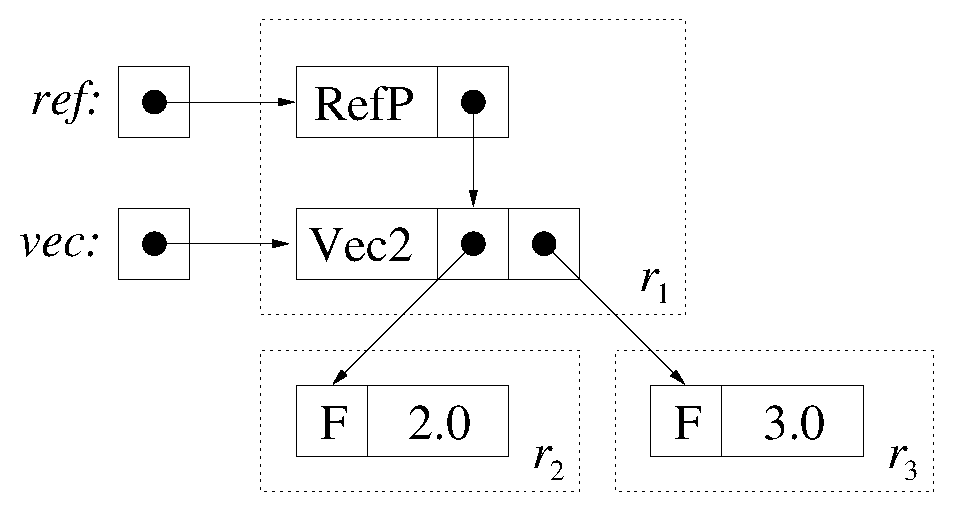
\includegraphics[scale=0.5]{2-System/fig/projections/pull-back}
\end{center}

We use the tag $\iRefP$ to record the fact that the $\iref$ object is a pull back reference that points into another object, as opposed to a regular ML style reference. When we execute the statement $\iref :=_{\#} 5.0$, it is the pointer inside the $\ivec$ object that is updated, not the $\iFloat$ object itself:

\begin{center}
\includegraphics[scale=0.5]{2-System/fig/projections/pull-back-update}
\end{center}

This leaves the old $2.0$ object to be reclaimed by the garbage collector.

The benefit of this system over ML style references is that we are able to update data structures without needing $\iRef$ in their type definitions, which addresses the refactoring problem discussed in \S\ref{intro:ref-types}. Note that in the above diagram, both the $\iVecTwo$ and $\iRefP$ objects are in the same region, $r_1$. This means that when we use a function like $(:=_{\#})$ to update the vector via the reference, the vector object will also be marked as mutable.

Although we don't \emph{need} ML style references, Disciple does support them, and we can equally define:

\code{
	$\kdata$ \ $\iVecTwo \ r_1 \ a = \iVecTwo \ \{ \ x :: \iRef \ r_1 \ a; \ y :: \iRef \ r_1 \ a \ \}$
}

In this case we would construct a vector with:

\code{
	$\ivec$		& $:: \iVecTwo \ r_1 \ (\iFloat \ r_2) \ (\iFloat \ r_3)$ \\
	$\ivec$		& $= \iVecTwo \ (\iRef \ 2.0) \ (\iRef \ 3.0)$
}

This produces the following objects in the store:

\begin{center}
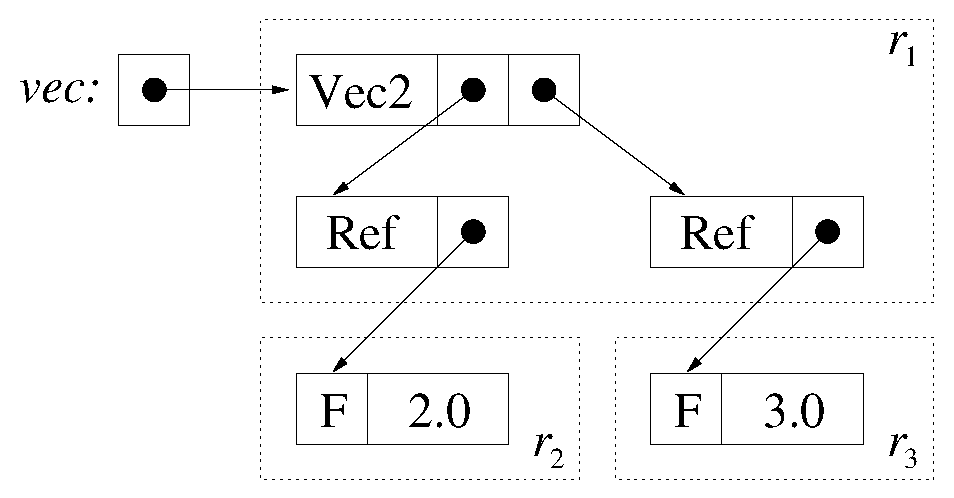
\includegraphics[scale=0.5]{2-System/fig/projections/vec-ref}
\end{center}

Here, the reference objects include the constructor tag $\iRef$, instead of $\iRefP$ as before. This indicates that to update these references, the pointer in the object itself should be modified, not the word that is pointed to.




\subsection{Custom projections}
\label{System:Projections:custom}

Along with the default field projections introduced by data type declarations, the programmer can also define their own custom projection functions. In fact, any variables they desire can be added to the name space associated with a type constructor, whether they are bound to functions that perform true projections, or not. For example, we can add a $\imagnitude$ function to the $\iVecTwo$ name space with:

\code{
	\mc{2}{$\kproject \ \iVecTwo \ \kwhere$} \\
		& $\imagnitude \ (\iVecTwo \ x \ y)$ \\
		& \qq $= \isqrt \ (\isquare \ x + \isquare \ y)$
}

We use $\odot \: \imagnitude$ to invoke this new projection. For example:

\code{
	$\kdo$	& $\ivec$	& $= \iVecTwo \ 2.0 \ 3.0$ \\
		& $\iputStr$	& $($``\texttt{The magnitude is:}" ++ $(\ishow \ \ivec \odot \imagnitude))$
}

Unlike default projections, custom projections can be defined to take extra arguments. For example, here is a projection to determine the dot product of two vectors:

\code{
	\mc{2}{$\kproject \ \iVecTwo \ \kwhere$} \\
		& $\idot \ (\iVecTwo \ \ixOne \ \iyOne) \ (\iVecTwo \ \ixTwo \ \iyTwo)$ \\
		& \qq $= \ixOne * \ixTwo + \iyOne * \iyTwo$
}

We can then use it as:

\code{
	$\kdo$	& $\ivec$	& $= \iVecTwo \ 2.0 \ 3.0$ \\
		& $\ivecTwo$	& $= \iVecTwo \ 4.0 \ 5.0$ \\
		& $\iputStr$	& $($``\texttt{The product is:}" ++ $(\ishow \ \ivec \ \odot \idot \ \ivecTwo))$
}

This allows a style of programming similar to using local methods in object oriented languages. For example, in Java we would write \texttt{vec.dot(vec2)}. With Disciple code, we find it helpful to view the projection $\odot \idot$ as a single operator. This highlights the similarities with the equivalent expression in vector calculus, $\ov{v_1} \bullet \ov{v_2}$.

Disciple also provides a punning syntax for adding variables to projection namespaces. This allows the programmer to add variables defined elsewhere in the module, and helps reduce the level of indenting in the code. For example, we could define our $\imagnitude$ and $\idot$ projections with:

\code{
	\mc{2}{$\kproject \ \iVecTwo \ \kwith \ \{ \imagnitude, \idot \}$} 
	\\[1em]
	$\imagnitude \ (\iVecTwo \ x \ y)$ \\
	\qq $= \isqrt \ (\isquare \ x + \isquare \ y)$ 
	\\[1em]
	$\idot \ (\iVecTwo \ \ixOne \ \iyOne) \ (\iVecTwo \ \ixTwo \ \iyTwo)$ \\
	\qq $= \ixOne * \ixTwo + \iyOne * \iyTwo$
}

We find this syntax useful when writing library code. Our usual approach is to define all the ``helper'' functions for a particular data type in the same module that declares it. These helper functions are present in the top level scope of the module, but are not exported from it directly. We use the punning syntax to add the helper functions to the projection namespace for the data type. We then export the data type name, and the projection namespace along with it. This allows us to write the majority of our program in the familiar Haskell style, while reducing the opportunity for name clashes between modules.
	


\clearpage{}
\section{Comparisons with other work}

% ---------------------------
\subsection{FX. 1986 -- 1993.\\
	Gifford, Lucassen, Jouvelot and Talpin.}

Although Reynolds \cite{reynolds:interference} and Popek \emph{et al} \cite{popek:euclid} had discussed the benefits of knowing which parts of a program may interfere with others, Gifford and Lucassen \cite{gifford:integrating} were the first to annotate a subroutine's type with a description of the effects it may perform. This allowed reasoning about effects in languages with first class functions, whereas previous work based on flow analysis \cite{banning:find-side-effects} was limited to first order languages. A refined version of their system is embodied in the language FX \cite{gifford:report-on-fx}, which has a Scheme-like syntax. We consider FX to be a spiritual predecessor of Disciple.

In Gifford and Lucassen's original system \cite{gifford:integrating}, the types of subroutines are written $\tau \to_C \tau$ where $C$ is an ``effect class'' and can be one of \scProcedure, \scObserver, \scFunction \ or \scPure. Subroutines marked \scProcedure \ are permitted to read, write and allocate memory. \scObserver \ allows a subroutine to read and allocate memory only. \scFunction \ allows a subroutine to allocate memory only. A subroutine marked \scPure \ may not read, write or allocate memory. Correctness dictates that subroutines marked \scPure \ cannot call subroutines marked \scFunction, those cannot call subroutines marked \scObserver, and they cannot call subroutines marked \scProcedure.

In this system, the concept of purity includes idempotence, and a subroutine that allocates its return value is not idempotent. Although such a subroutine cannot interfere with other parts of the program, the fact that it might allocate memory must be accounted for when transforming it. We will return to this point in \S\ref{Core:Optimisation:floating-out}. Note that in Disciple we use quantification of region variables to track whether a function allocates its return value, and our definition of purity includes functions that do so.

In \cite{lucassen:polymorphic-effect-systems} Gifford and Lucassen introduce the polymorphic effect system. This system includes region variables, quantification over region and effect variables, and effect masking. The primitive effects are $\iRead \ r$, $\iWrite \ r$ and $\iAlloc \ r$, and $e_1 \lor e_2$ is written \texttt{maxeff} $e_1 \ e_2$. Their language uses explicit System-F style type, region and effect abstraction and applications, which makes their example programs quite verbose. Their system also includes region unions, where the region type \texttt{union} $r_1 \ r_2$ represents the fact that a particular object may be in either region $r_1$ or region $r_2$. Disciple does not yet include region unions as they complicate type inference. This point is discussed in \S\ref{Evaluation:Limitations:blocked-regions}.

In \cite{jouvelot:reconstruction-types-and-effects} Jouvelot and Gifford describe an algebraic reconstruction algorithm for types and effects. They separate type schemes into two parts, the value type and a set of effect constraints, which gives us the familiar $\forall \ov{a}. \ \tau \rhd \Omega$ for type schemes. Here, $\ov{a}$ is a collection of type variables, $\tau$ is the body of the type and $\Omega$ are the constraints. On the other hand, the left of the constraints in their work can be full effect terms, not just variables. They present a proof of soundness, but only a single example expression. They also remark that they were still working on the implementation of their system in FX, so its practicality could be assessed.

In \cite{talpin:polymorphic} Talpin and Jouvelot abandon the explicit polymorphism present in previous work, require the left of effect constraints to be a variable, and introduce sub-effecting. This allows their new system to have principle types. Sub-effecting is also used to type if-expressions, as the types of both alternatives can be coerced into a single upper bound. Finally, in \cite{talpin:discipline} they present the Type and Effect Discipline and address the problem of polymorphic update \S\ref{System:PolyUpdate}. They use effect information to determine when to generalise the type of a let-bound variable, instead of relying on the syntactic form of the expression as they did in \cite{jouvelot:reconstruction-types-and-effects}. We have based Disciple on this work.


% ---------------------------
\subsection{C++ 1986 \\Bjarne Stroustrup. }
The C++ language \cite{stroustrup:cpp, cpp-standard} includes some control over the mutability of data. In C++ a pointer type can be written \texttt{*const}, which indicates that the data it points to cannot be updated via that pointer. Pointers can also be explicitly defined as mutable. Fields in structures and classes can be defined as either mutable or constant, though they default to mutable due to the need to retain backwards compatibility with C. C++ also provides some limited control over side effects whereby a \texttt{const} qualifier can be attached to the prototype of a class method. This indicates that it does not (or at least should not) update the attributes of that class. However, this can be circumvented by an explicit type cast, or by accessing the attribute via a non-const pointer.

\texttt{const} annotations are also supported in C99 \cite{c99-standard}. Some C compilers including GCC \cite{gcc-4.3.2} provide specific, non-standard ways to annotate function types with mutability and effect information. For example in GCC the programmer can attach a purity attribute to a function that allows the optimiser to treat it as being referentially transparent. Attributes can also be added to variables to indicate whether or not they alias others. Of course, these attributes are compiler pragmas and not checked type information, and neither C++ or C99 has type inference. With DDC we can infer such information directly from the source program, and the type system for our core language ensures that it remains valid during program transformation. 

More recent work based on Java  \cite{birka:reference-immutability} can ensure that \texttt{const} qualified objects remain constant, and \cite{foster:type-qualifiers} presents a general system of type qualifiers that includes inference. However, neither of these systems include region or effect information, or discuss how to add qualifiers to Haskell style algebraic data types. In \cite{foster:type-qualifiers} the authors mention that some effect systems can be expressed as type qualifier (annotation) systems, but state that the exact connection between effect systems and type qualifiers was unclear. In this chapter we have shown how to re-use Haskell's type classing system to qualify both region and effect information, which brings regions, effects and qualifiers into single framework. 


 
% ---------------------------
\subsection{Haskell and unsafePerformIO. 1990 \\Simon Peyton Jones \emph{et al}. }
	
The Haskell Foreign Function Interface (FFI) \cite{haskell-ffi} provides a function \\ $\iunsafePerformIO$ that is used to break the monadic encapsulation of IO actions. It has the following type:

\code{
	$\iunsafePerformIO$ :: $\iIO a \to a$ 
}

Use of this function discards the guarantees provided by a pure language, in favour of putting the programmer in direct control of the fate of the program. Using $\iunsafePerformIO$ is akin to casting a type to \texttt{void*} in C. When a programmer is forced to use $\iunsafePerformIO$ to achieve their goals, it is a sign that the underlying system cannot express the fact that the program is still safe. Of course, this assumes the programmer knows what they're doing and the resulting program actually \emph{is} safe.

As Disciple includes an effect system which incorporates masking, the need for a function like $\iunsafePerformIO$ is reduced. As discussed in \S\ref{System:Effects:masking}, if a particular region is only used in the body of a function, and is not visible after it returns, then effects on that region can be masked. In this case the system has proved that resulting program \emph{is} actually safe. 

On the other hand functions like $\iunsafePerformIO$ allow the programmer to mask top level effects, such as $\iFileSystem$. For example, we might know that a particular file will not be updated while the program runs, so the effect of loading the file can be safely masked. In these situations the type system must always ``trust the programmer'', as it cannot hope to reason about the full complexity of the outside world.


% ---------------------------
\subsection{Behaviors and Trace Effects. 1993 \\ Nielson and Nielson \emph{et al}}

In \cite{nielson:from-cml-to-its-process-algebra} Nielson and Nielson introduce \emph{behaviours}, which are a richer version of the FX style effect types. As well as containing information about the actions a function may perform, behaviours include the order in which these actions take place. They also represent whether there is a non-deterministic choice between actions, and whether the behaviour is recursive. Having temporal information in types can be used to, say, enforce that files must be opened before they are written to. Skalka \emph{et al}'s recent work \cite{skalka:trace-effects} gives a unification based inference algorithm for a similar system. For Disciple, we have been primarily concerned with optimisation and have so far avoided adding temporal information to our effect types. However, we expect that Disciple's main features such as mutability inference and purity constraints are reasonably independent of temporal information, and adding it represents an interesting opportunity for future work.


% ---------------------------
\subsection{$\lambda_{\ivar}$. 1993 -- 1994 \\ Odersky, Rabin, Hudak, Chen}
In \cite{odersky:lambda-var} Odersky, Rabin and Hudak present an untyped monadic lambda calculus that includes assignable variables. Interestingly, their language includes a keyword $\kpure$ that provides effect masking. $\kpure$ is seen as the opposite of the monadic $\kreturn$ function. This work is continued in Rabin's thesis \cite{rabin:functional-assignment}. The Imperative Lambda Calculus \cite{swarup:assignments-applicative, yang:ilc-revisited} is a related system. 

In \cite{chen:type-lambda-var} Chen an Odersky present a type system for $\lambda_{\ivar}$ to verify that uses of $\kpure$ are safe. This is done by stratifying the type system into two layers, that of pure expressions and that of commands. Their inference algorithm uses a simple effect system that does not distinguish between pure and impure lambda bound functions. They note that using the region variables of Talpin and Jouvelot's system \cite{talpin:polymorphic} would give better results. 


% ---------------------------
\subsection{MLKit. 1994 \\Tofte, Talpin, Birkedal}
MLKit \cite{tofte:mlkit-4.3.0}, uses regions for storage management, whereas DDC uses them to help reason about the mutability and sharing properties of data. In MLKit, region annotations are only present in the core language. As in DDC, MLKit supports region polymorphism, so functions can be written that accept their arguments from any region, and output their result into any region. Unlike DDC, MLKit adds region annotations to function types, as the runtime objects that represent functions are also allocated into regions. 

MLKit performs type inference with a two stage process \cite{tofte:region-inference}. The SML typing of the program is determined first, and region annotations are added in a separate analysis. This helps when performing type inference in the presence of polymorphic recursion, which is important for storage efficiency. Although polymorphic recursion of value types is known to make the general type inference problem undecidable \cite{mycroft:polymorphic-recursion}, in MLKit it is supported on the region information only, via a fixed point analysis. As DDC does not use regions for storage management, polymorphic recursion is not as important, and we do not support it.


% ---------------------------
\subsection{Functional Encapsulation. 1995. Gupta}
\label{System:Comparisons:functional-encapsulation}

In \cite{gupta:functional-encapsulation} Gupta presents a system to convert mutable objects to constant ones for the parallel language Id. As discussed in \S\ref{System:Effects:masking} this is needed for objects that are constructed imperatively, but are used functionally thereafter. Like our own system, Gupta's is based on Leroy's closure typing \S\ref{System:Closure}. He presents a term $\kclose \ t_1$ whose result has the same value as $t_1$, except that the type system statically enforces that it will no longer be updated. The type of $\kclose \ t_1$ can also be generalised, because the return value is guaranteed not to suffer the problem of polymorphic update \S\ref{System:PolyUpdate}. $\kclose$ is interesting because it serves as the dual of the \emph{effect} masking operator, $\kpure$, which appears in $\lambda_{\ivar}$ \cite{odersky:lambda-var}.

As in our own system, Gupta uses region variables to track the mutability of objects. Instead of using region constraints, region variables are only attached to the types of mutable objects. All constant objects are annotated with the null region $\epsilon$. 

In his conclusion, Gupta laments that $\kclose$ had not yet been implemented in the Id compiler, and it still relied on ``hacks''. The Id language was reincarnated as a part of pH \cite{nikhil:ph}, but $\kclose$ did not make it into the language specification. Being based on Haskell, it ended up using state monads to provide its impure features. Although we have not yet implemented mutability masking in DDC, it is a highly desirable feature and is first in line for future work \S\ref{Evaluation:Limitations:mutability-masking}.


% -------------------------------------
\subsection{Objective Caml. 1996 \\
	Leroy, Doligez, Garrigue, R\'{e}my and J\'{e}r\^ouillon.}

As well as $\iRef$ types, O'Caml \cite{leroy:ocaml-3.11} supports mutable record fields. In fact, the $\iRef$ constructor is expressed as a record with a single mutable field. Mutable fields are declared with the $\kmutable$ keyword. Fields that are not declared as mutable default to constant. Mutable fields are updated with the $\leftarrow$ operator. The following example is from the O'Caml 3.11 manual:

\code{
	$\ktype \ \imutableUpoint$ 
			& $= \{ \kmutable \ x: \ \ifloat; \ \kmutable \ y: \ifloat \};;$ 
	\\[1ex]
	$\klet \ \itranslate \ p \ dx \ dy $
			& $= \ p.x \ \leftarrow \ p.x + dx; \ p.y \leftarrow p.y + dy;;$
}

One of the benefits of mutable record fields over $\iRef$ types is that we do not need to sprinkle calls to $\ireadRef$ throughout our code. This reduces the refactoring effort required when the mutability of an object is changed. However, unlike Disciple, O'Caml does not support mutability polymorphism, so two records that have the same overall structure but differ in the mutabilities of their fields have incompatible types. A constant list has a different type to a mutable list, and the standard O'Caml libraries only provide the constant version. This point was also discussed in \S\ref{intro:ref-types}.


% -------------------------------------
\subsection{Calculus of Capabilities and Cyclone. 1999 \\ Crary, Walker, Grossman, Hicks, Jim, and Morrisett}
\label{System:Comparisons:CalculusOfCapabilities}

Cyclone \cite{jim:cyclone} is a type-safe dialect of C which uses regions for storage management. Its type system derives from Crary, Walker and Morrisett's work on the Calculus of Capabilities \cite{crary:capabilities}. The Vault \cite{deline:vault} and RC \cite{gay:rc} languages are related.

Cyclone's type safety is achieved in part by using region typing to track the lifetimes of objects, and to ensure that programs do not dereference dangling pointers \cite{grossman:region-cyclone}. Cyclone has region polymorphism and parametric value polymorphism \cite{grossman:quantified-imperative}, but not mutability polymorphism. Being an imperative style language, programs tend to be expressed using update and pointer manipulation. Allocation is explicit, though deallocation can be performed via the region system, or implicitly via garbage collection.

As in C, higher order functions can be introduced using function pointers. Cyclone supports existential types, and these can be used to express type safe function closures. Cyclone does not support full Hindley-Milner style type reconstruction, but instead relies on user provided type annotations. Region annotations are attached to pointer types in the source language, though many annotations can be elided and subsequently reconstructed by using intra-function type inference and defaulting rules.

The main technical feature that the Calculus of Capabilities (CC) has over the DDC core language is that the capability to perform an action can be revoked. The CC can then statically ensure that that a revoked capability is no longer used by the program. This mechanism is used in Cyclone's region system, where the capability to access a particular region is revoked when the region is deallocated. In contrast, in DDC a capability such as the ability to update a region cannot be revoked by the programmer. We have discussed mutability masking in \S\ref{System:Effects:masking}, but have not implemented it. On the other hand, DDC supports full type inference (apart from ambiguous projections, which are an orthogonal issue).

Although Cyclone is an imperative language, its use of regions in the source language means that it shares some common ground with Disciple. For example, here is the type of sets from \cite{grossman:region-cyclone}:

\code{
	\mc{2}{\texttt{struct \ Set<}$\alpha, \rho$\texttt{> \{}} \\
	& \texttt{list\_t <}$\alpha, \rho$\texttt{> elts;} \\
	& \texttt{int (*cmp)(}$\alpha, \alpha;$\ \texttt{regions\_of(}$\alpha$\texttt{));} \\
	\texttt{\}}
}

The $\rho$ annotation is the primary region variable and $\alpha$ is a type variable. The term \texttt{regions\_of(}$\alpha$\texttt{)} is an effect that represents the fact that the comparison function \texttt{cmp} on two values of type $\alpha$ could access any region contained in that type. In this respect \texttt{regions\_of(}$\alpha$\texttt{)} has the same meaning as $\iReadT a \lor \iWriteT a$ from \S\ref{System:TypeClassing}. Note that as Cyclone is based on C, most data is mutable. In such a language there is less to be gained by separating effects on regions into reads and writes. A general region access effect suffices.


% ---------------------------
\subsection{BitC. 2004 
	\\ Shapiro, Sridhar, Smith, Doerrie}

BitC \cite{shapiro:bitc-language-specification} is a Scheme-like language targeted at systems programming. One of its stated aims is to offer \emph{complete mutability}, meaning that any location -- whether on the stack, heap or within unboxed structures -- can be mutated \cite{sridhar:type-inference-systems-language}. BitC supports the imperative variables that we decided not to in \S\ref{System:Update}. 

The operational semantics of BitC includes an explicit stack as well as a heap, and the arguments of functions are implicitly copied onto the stack during application. This allows the local copies to be updated in a way that is not visible to the caller, a behaviour demonstrated by the following C program:
\begin{lstlisting}
int fun(int x)
{
     x = x + 1;
     return x;
}
\end{lstlisting}

BitC includes mutability inference, and inferred type for the BitC version of \texttt{fun} will be:
\begin{lstlisting}
(mutable int) -> (mutable int)
\end{lstlisting}
Note that the fact that \texttt{x} is updated locally to \texttt{fun} has ``leaked'' into its type. We do not actually need to pass a mutable integer to \texttt{fun}, because only the fresh copy, located in the stack frame for the call, will be updated. For this reason, BitC introduces the notion of \emph{copy compatibility}, which is similar to the property expressed by our $\iShape$ constraint from \S\ref{System:TypeClassing:copy-and-update}. We can pass a \mbox{\texttt{const int}} to a function expecting a \texttt{mutable int}, because the first will be implicitly copied during the call.

Although \cite{shapiro:origins-of-bitc} discusses adding effect typing to BitC, it does not mention region variables, so the possible effects are limited to the coarse-grained \emph{pure}, \emph{impure} and \emph{unfixed}. Exploiting effect information during program optimisation is not discussed, and the more recent formal specification of the type system in \cite{sridhar:formalization-of-bitc-type-system} does not include it. 


% ---------------------------
\subsection{Monadic Regions. 2006
	\\ Fluet, Morrisett, Kiselyov, Shan}

In \cite{fluet:monadic-regions} Fluet and Morrisett draw on the MLKit and Cyclone work to express a version of the region calculus in a monadic framework. Once again, they focus on using regions for storage management. They trade complexity of the original region type system for complexity of encoding, though the result could serve as a useful intermediate language.



